\documentclass[11pt]{article}
\usepackage{geometry}
\geometry{left=1.1in,right=1.1in,top=1.1in,bottom=1.1in}

\usepackage{amsmath,amssymb}
\usepackage{graphicx}
\usepackage{booktabs}
\usepackage{float}
\graphicspath{{./}{../output/}}
\usepackage{setspace}
\usepackage[utf8]{inputenc}
\usepackage[semicolon]{natbib}
\usepackage{enumitem}
\usepackage[table]{xcolor}
\usepackage{hyperref}

\onehalfspacing
\setlength{\parindent}{22pt}
\setlength{\parskip}{5pt}

\definecolor{darkred}{rgb}{0.64, 0, 0}
\hypersetup{colorlinks=true, citecolor=darkred, filecolor=darkred, linkcolor=darkred, urlcolor=darkred}

\begin{document}

\title{The Insurer Is Hit Too: Joint Job Loss of Spouses\ and the Limits of Family Insurance
\thanks{\footnotesize Preliminary draft.}}
\author{Jiaqi Li \ University of Sheffield}
\date{\today}
\maketitle

\begin{abstract}
\noindent When a husband loses his job, his wife is ten times as likely to lose hers in the same month. In thirty years
of the Current Population Survey, among 1.3 million married couples in which both spouses work, the wife's monthly
job-loss probability is 5.45\% in the month her husband loses his job against 0.54\% otherwise; the excess survives state
$\times$ month $\times$ industry fixed effects, is present in all 51 states, is larger in recessions, and is the same in Black and White couples. It is carried by the workplace: a shared employer accounts for a third to a half of the excess, and couples in the same industry for more than half of it. With each spouse's own reason for the
job ending, the Displaced Worker Supplement and the PSID confirm the fact, the SIPP replicates it month by month, and the PSID
splits it into a permanent part, couples who share risk, and a larger
contemporaneous part. The joint loss is small in the household's average income loss but large in the month of the
shock: wives who were not working search at once and find jobs slowly, so average added-worker estimates, which net
the wives who add work against the wives who lose their own jobs, understate what wives do and overstate what families
can absorb. Job loss also strains the marriage this insurance relies on: a wife's own job loss ends marriages as
often as her husband's, and a joint loss most often. The fact ranks the safety net: an earnings subsidy such as the Earned Income Tax Credit pays nothing in the
months in which both spouses are out of work, while food stamps, which rise after displacement, pay in every state. I set out a
two-earner model with correlated displacement risk, estimated on these moments, to measure what undiversified family
insurance does to consumption, to children and to the ranking of work-conditioned and unconditional transfers.
\end{abstract}

\clearpage

\section{Introduction}\label{sec:introduction}

Families insure themselves against job loss. When a husband loses his job, his wife can work more, and this added
worker effect is a central part of the insurance a family has before it draws on savings and public transfers
\citep{lundberg1985added,cullen2000does,stephens2002worker,shore2010better,halla2020job,birinci2019spousal,mankart2017household,bacher2025joint}.
The leading estimate is that of \citet{blundell2016consumption}: family labor supply provides 63\% of the insurance
against permanent shocks to the husband's wage, the government 20\% and savings 17\%; rerunning their code, I
reproduce their estimates exactly. That insurance needs two things the estimate takes as given: a second earner whose
job is not lost with the first, and a marriage that survives the shock. This paper shows that neither can be taken as
given. When a husband loses his job, his wife is ten times as likely to lose hers in the same month; the household is
then left with no earner, and in those months the Earned Income Tax Credit, designed to support the most vulnerable
working families, pays it nothing, because it pays only on earnings and only once a year. And a job loss of either spouse ends marriages
\citep{charles2004job}, most often when both spouses lose their jobs.

Why has this been missed? \citet{ganong2026earnings} show that most US workers' pay moves substantially from month to
month, that the movements come largely from hours set by firms rather than from wages, and that they are transitory
enough to be masked in annual data; they set aside unemployment and job changes, which, they note, would only add to
the instability. This paper studies that margin at the level of the household: the job itself is lost, and both
spouses lose theirs together. The two literatures meet here. In the two-year changes of
\citet{blundell2016consumption}, joint displacements are 0.3\% of couple-years, too rare for an estimator built on
average covariances to see, while in monthly data they occur ten times as often as independent risks imply. And if
hours and jobs are set by firms, part of what an annual framework reads as the second earner's insurance response is a
shock to the second earner: family insurance is weakest in the month of the shock.

The fact is measured to the month. In thirty years of the Current Population Survey (CPS), 1.3 million married couples in which both spouses work, a wife loses her job in
5.45\% of the months in which her husband loses his and in 0.54\% of the months in which he keeps it. The excess, 4.0
percentage points (standard error 0.002), is the same when couples are compared within the same state and month and
when wives are compared within the same state, month and industry (3.7 points), so it is not the local business cycle.
It is present in all 51 states, larger in recessions, and concentrated where spouses share a workplace: in the same
detailed industry, 23\% of wives lose their job in the month their husband does. A shared employer carries a third
to a half of the excess: couples in the same detailed industry, occupation and class of worker, the closest the public
data come to a common employer, account for about a third of it, and couples in the same industry for more than half. It is not an artefact of who reports
(3.8 points whether the wife or the husband reports the other's job loss), of temporary layoffs (2.7 points without
them) or of the season, and a joint permanent job loss---both spouses still unemployed two months later---is 13 times as
likely in the month the husband loses his job as in other months.

The fact and the estimate of \citet{blundell2016consumption} are not in conflict. Their shocks are innovations to the
hourly wages of husbands who keep working, in couples who stay together, while a job loss changes partners: the share
of displaced fathers still living with their wife falls by 4.5 percentage points within three years for Black fathers
and by 1.9 points for White fathers. Two omissions bear on the safety net: the Earned Income Tax Credit in their
schedule pays nothing in the state in which both spouses have lost their jobs, which a framework built on positive
hours does not contain, and the families who rely most on food stamps are largely outside the sample, although 71\% of
the insurance of the food-stamp-eligible households who remain comes from the government. Family labor supply insures
the wage shocks of stable, continuously employed couples; it fails against the shock at which the second earner's job
is lost with the first---which is why the joint job loss matters for the design of welfare programs.

The closest model is the joint search model of \citet{bacher2025joint}. In CPS couples in which one spouse works and the
other does not, they find that the non-working spouse is 5.6 percentage points more likely to enter the labor force
when the working spouse loses his job, 7.1 points at ages 26--35 and 1.4 points at 56--65, and they explain the decline
with age in a monthly life-cycle model of two spouses who search jointly, save and accumulate human capital, with
unemployment insurance. Their evidence concerns the spouse who can enter work; this paper concerns the spouse who is
lost, in couples in which both work. Separation shocks in their model are independent across spouses, and they note
that correlated shocks, from couples sorting into the same industries and occupations, are left out. With independent
risks, the probability that both spouses lose their jobs in the same month is close to the product of their separate
risks, about a tenth of what the CPS shows, so a model of that kind understates by construction the state in which the
household has no earner. This paper measures the correlation and builds it into a model with the structure of
\citet{bacher2025joint}: the spouses' displacement risk has a common component, larger for couples who share an employer
or an industry, and a permanent component for couples who share risk; the safety net includes the Earned Income Tax
Credit and food stamps as well as unemployment insurance; the marriage can end after a job loss; and all parameters are
estimated jointly. In the same CPS panel I reproduce their added worker effect (5.6 points) and its decline with age, from 6--7 points
before 45 to 1.2 points at 56--62; the joint job loss of spouses who both work does not decline with age (an excess of
2.8 points at 26--35 and 2.7 at 56--62 outside temporary layoffs). The spouse who can enter work is available mainly
when young; the spouse who is lost is lost at every age.

Family insurance is undiversified: a wife's job-loss hazard rises tenfold in the month her husband loses his job, the
excess is carried by shared workplaces rather than the local cycle, and because the second earner is lost exactly
when she is needed, average added-worker estimates understate what wives do and overstate what families can absorb; a
two-earner model with correlated displacement risk is built to show what this does to consumption, children and the
ranking of work-conditioned versus unconditional transfers.

The joint job loss is the paper's headline. It changes how the added-worker literature should be read and how family
insurance should be modelled. It is not itself a result about children or intergenerational mobility: children and
mobility are the stakes, which the model delivers.

The paper follows the shock in the order in which it reaches the family. Section~\ref{sec:jointloss} establishes the
fact. The CPS measures it to the month: the wife's excess risk is 0.6--0.7 points in the two months before her
husband's job loss, 4.0 points in the month of it and 0.6--0.8 points in the two months after. The Panel Study of
Income Dynamics (PSID) measures it with each spouse's own reason for the job ending. Around a husband's displacement
his wife's own displacement rises by 5.2 percentage points, from a base of 5.8\%; about 2 points of this are a
permanent trait of couples who share risk, since wives of men who will be displaced six to ten years later are already
more often displaced, and 3 points are contemporaneous. The shocks are shared at the workplace. The wife's own employer
closes in the year her husband's does, and the excess is 20 points larger when the spouses work in the same sector and
28 points larger in the same three-digit industry. It does not move with the local unemployment rate. The tetrachoric
correlation of the spouses' job losses is 0.24, and 0.50 when they share a sector. The CPS Displaced Worker
Supplement, 1984--2024, which records each adult's reason for a job loss in 417,269 couples, gives the same answer: a
wife is 4.3 times as likely to be displaced in the year her husband is, joint plant closings are almost ten times as
frequent as independent closings would imply within the same year, and the excess is the same in both races; and the
SIPP, which follows 50,692 couples month by month, gives a same-month ratio of 7.7.

Section~\ref{sec:household} asks what the household loses and what it does. A husband's displacement lowers his labor
income by 17\% (Black fathers) to 24\% (White fathers) over the following three years and family income by at least as
much. Wives work 51 more hours a year on average, 112 more when the youngest child is under six. Wives who were not
working start looking for work at once, but their employment takes about six months to build up. In the CPS the
probability that they are unemployed and looking rises by 8.8 points in the month after their husband's job loss, while
their employment rises by 2.2 points after one month and 4.2 after three; in the SIPP, which follows them for three
years, looking for work jumps at once and employment builds from 1.9 points in the month of the husband's separation to
5.4 points after six months. In the month in which the household's income falls most, its second earner is
more likely to lose her own job than to add work. This is the timing that average added-worker estimates miss: they
net the wives who work more against the wives who lose their own jobs to the same shock. The joint loss is small in
the household's average income loss (about \$260 a year, 2\% of the family's loss) but large where it bites, in the
month of the shock and among couples who share a sector, and it is absent from models of family insurance. The job
loss also strains the marriage: the share of displaced fathers still living with their wife falls by 4.5 percentage
points within three years for Black fathers and 1.9 points for White fathers. The wife's own job loss is followed by
break-up as often (4.6 points within three years, not different from the husband's), so a job loss on either side can
end the arrangement that is meant to insure it, although part of the response after her layoffs may reflect who is
laid off. Food stamp receipt rises by about four
points; AFDC/TANF barely moves.

Which part of the safety net can insure the family follows from the joint job loss. The Earned Income Tax Credit, the
largest cash transfer to families with children, pays only when someone in the household works, so it fails exactly
when both spouses lose their jobs; programs that do not require earnings, such as food stamps, are the ones that can
insure the family in that state. Section~\ref{sec:children} reports what the PSID can say about the children: children
of displaced fathers reach lower incomes and less schooling as adults, but displaced families were worse off before the
job loss, and the associations are robust only for White children's schooling. The paper uses them as bounds, not as
estimates of the effect. Section~\ref{sec:model} sets out a two-earner model with correlated displacement risk, a
search friction, savings, the marriage and the safety net, estimated on these moments, and the policy experiments that
the correlation makes informative: correlated against independent shocks, unemployment insurance for both spouses, an
earnings subsidy against an unconditional transfer of equal cost, and childcare.

The paper makes four contributions. The first is the fact: family insurance is undiversified, because the second
earner's job is lost to the same shock and in the same month as the first earner's; the excess is measured to the month
in the CPS and with each spouse's own reason for the job ending in the PSID, it is carried by shared workplaces, and it
is equal in both races. The second is what the fact implies for the added-worker literature
\citep{cullen2000does, stephens2002worker, halla2020job}: average estimates net the wives who work more against the
wives who lose their own jobs, so they understate what wives do and overstate what families can absorb in the month of
the shock. The third concerns the marriage that the insurance relies on. A job loss of either spouse raises
divorce \citep{charles2004job}, and studies of job loss follow one displaced worker at a time
\citep{eliason2012lost, athey2026heterogeneous}. Measuring both spouses' losses on one sample with one design, I
confirm over 1984--2021 that the wife's own job loss ends marriages as often as her husband's, and show that the
response is largest when both spouses lose their jobs (9.5 points fewer couples still together six years on, against
4.1 points when only he loses his). The fourth carries the facts into a
model of family insurance \citep{birinci2019spousal}, which is built to measure what undiversified insurance does to
consumption, to children and to the ranking of work-conditioned transfers against unconditional ones. Section~\ref{sec:literature} sets out what is known and what is new.

Race enters as a dimension of heterogeneity. Black men lose their jobs more often (8.0\% a year against 4.8\% for
White men in the PSID) and are the first to lose them when the economy weakens \citep{couch2010last}, and Black families
hold far less wealth \citep{derenoncourt2023wealth}, so the household's insurance matters more for them. The joint job
loss itself is the same in both races (an excess of 4.4 points for Black and 3.8 points for White couples in the CPS;
difference $p=0.309$); the separation response is larger in point estimate for Black families but not significantly so; and Black wives who were not working add less work
after their husband's job loss.

Appendix~\ref{app:other} reports evidence that bears on the model's assumptions but not on the headline: around a birth,
mothers' work does not respond to shocks to their husbands' industries (a precise null), mothers' work in a child's
first year is not associated with worse child outcomes in these data, and slack labor markets lower rather than raise
mothers' employment after a birth. Appendix~\ref{app:designs} reports the designs that did not identify what they were
meant to.

\section{Related Literature}\label{sec:literature}

\paragraph{The joint labor-market risk of spouses.} That spouses' outcomes are linked is known. Their earnings covary,
mostly through permanent components \citep{hyslop2001rising}, more so in booms \citep{shore2010better}; couples sort on
employer and industry, and about a tenth of dual-earner couples work at the same establishment
\citep{hyatt2019coworking}; displacement studies observe couples displaced by the same plant event and drop them
\citep{halla2020job}; and correlated unemployment has been offered as one of two explanations for the small
added-worker response in the United States \citep{kawano2025who}. What has not been measured is the joint job loss
itself: how much a husband's job loss raises his wife's own job-loss hazard, when, and through which channel.
Table~\ref{tab:contribution} sets out what is known and what this paper adds.

\paragraph{Insurance within the household.} Wives' earnings fall by up to 73 cents for each dollar of unemployment
insurance their husbands receive \citep{cullen2000does}. In the PSID, wives' labor supply rises after a husband's
displacement, slowly, replacing more than a quarter of his lost income in the long run \citep{stephens2002worker};
family labor supply is a main channel of insurance against permanent wage shocks \citep{blundell2016consumption}. In
Austria, wives replace a very small share of the household's loss, public transfers and taxes do more, and young
children shape the response \citep{halla2020job}. \citet{birinci2019spousal} attributes the small US response to
crowding out by transfers and, in a model with a frictional labor market and family labor supply, finds that optimal
policy shifts transfers from means-tested to employment-tested; \citet{mankart2017household} also model household
search as insurance. \citet{bacher2025joint} show in CPS couples that a non-participating spouse is 5.6 percentage points more likely to
enter the labor force when the primary earner loses his job, 7.1 points at ages 26--35 and 1.4 at 56--65, and explain
the decline with age in a monthly life-cycle model of joint search with assets, human capital and unemployment
insurance; separation shocks in their model are independent across spouses, and they note that correlated shocks,
from sorting into the same industries or occupations, are left out. This literature treats the wife's job as given
when the husband's is lost. This paper adds the
second earner's own risk and its timing.

\paragraph{Why another paper after \citet{blundell2016consumption}.} The closest paper is
\citet{blundell2016consumption}, who estimate a life-cycle model of two earners with correlated permanent and
transitory wage shocks, nonseparable preferences and a progressive tax and transfer schedule that includes the Earned
Income Tax Credit and food stamps, on PSID consumption, earnings and assets for 1999--2009. A 10\% permanent fall in the
husband's wage lowers consumption by 3.2\%; of the 39 percentage points of consumption that are insured, 63\% are insured
by family labor supply, 20\% by taxes and transfers and 17\% by savings, and a parameter for insurance outside these
channels is not different from zero ($-0.137$, s.e.\ 0.270). The spouses' transitory wage shocks are correlated (0.31),
their permanent shocks are not (covariance 0.0027, s.e.\ 0.0023). Read at face value, the wife is the household's main
insurer; this paper finds that, against job loss, she largely is not.

I rerun their code on their PSID panel (Appendix~\ref{app:bps}). Every point estimate is reproduced
(Table~\ref{tab:bps_relax}, column 1), and the result does not rest on most of their sample choices. Their
controls for both spouses' employment status do not affect the accounting, although they matter at the event itself
(the wife's earnings residual in the interval of her own displacement is $-0.10$ with them and $-0.20^{***}$ without);
adding the PSID's low-income sample raises the share of family labor supply to 0.68. The authors note that dropping
husbands with long spells without work may understate or overstate added-worker effects
\citep[p.~403]{blundell2016consumption}; dropping only the year without work, rather than the husband's whole record,
measures this and lowers the family share from 0.62 to 0.56. The estimator itself is sensitive to the trim of years of
collapse and recovery, a standard treatment of measurement error, which removes almost no displacement years.\footnote{Code:
\texttt{IGE/bps\_reconciliation/} (copies of their do-files with every edit listed in \texttt{README.md}). The 1999
early-release income file needed to rebuild their panel from the raw PSID is not public, so the replication starts from
their constructed panel, which their own code reproduces exactly.}

The difference lies in the shock and in how often it occurs. Their shocks are innovations to the hourly wages of
husbands who keep working, measured as annual earnings over annual hours in two-year changes; a job loss appears as a
fall in hours, and a coincidence of two job losses within a month cannot be seen. High-frequency administrative data
show that this is where most earnings risk lies: \citet{ganong2026earnings} find, with payroll and bank-account records,
that in three quarters of months a worker's pay differs from the month before and in a quarter of months by at least
17\%, that the changes come from hours rather than wages, that about half of a typical worker's hours volatility is caused
by firm-level fluctuations in total hours, that lower-income hourly workers face the most, that the volatility raises
consumption volatility for workers with little liquidity, and that it is masked in annual data. Their analysis stays
within ongoing jobs and studies workers rather than couples; the joint job loss is the household-level counterpart across
jobs, a firm-driven fall of both spouses' hours to zero in the same month. In the panel of
\citet{blundell2016consumption}, a husband is displaced in 4.4\% of couple-years and both spouses in 0.3\% (28
couple-years); of 57 joint displacements among married couples with husbands aged 30--57, 28 reach their estimation file
and 17 contribute a wage moment (Table~\ref{tab:bps_attrition}), most of the rest lost to the exclusion of the
low-income sample, missing lagged observations and the requirement that husbands work in every year. An estimator built
on average covariances of wage, earnings and consumption growth cannot see an event this rare, and their transitory
wage covariance is not carried by displacement years (0.0063 without them). In the interval of a joint displacement the
husband's earnings fall by 0.335 against 0.123 after a single displacement, and the wife's earnings by an arc change
0.44 larger; consumption does not fall in that interval but falls by more in the following one after a joint than after
a single displacement (Table~\ref{tab:bps_event}: $-0.138^{**}$ with the low-income sample, $-0.071$, $p=0.19$, in their
sample). With 17 to 23 joint events this is suggestive; Section~\ref{sec:household} reports the consumption response in
the full PSID for 1999--2021.

Three further features matter for the comparison. The insurance that family labor supply provides in their accounting
is the wife's hours response, a Marshallian cross-elasticity of $-0.75$ identified from wives who work in both years of
the interval, in couples in which the husband keeps working. Applied to a displaced husband's permanent wage loss of
15--20\%, it implies 190--250 more hours a year from wives who already work; on the extensive margin their estimates imply
that 8.4\% of non-working wives enter work per 10\% permanent fall in the husband's wage, or 13--17\% after a displacement
\citep[p.~428]{blundell2016consumption}. The responses to displacement measured here are smaller: 51 hours a year on
average in the PSID and, from 1984, a gross 47 hours offset by 35 hours of joint job losses, and 4.2 (CPS) to 5.4 (SIPP)
percentage points more employment among wives who were not working. The record of a couple ends when the spouse
changes, and the job loss itself changes partners, so a sample of stable couples keeps the households in which the
marriage survived the shock. And the safety net in their schedule is a function of positive family earnings with no
unemployment insurance: the Earned Income Tax Credit pays nothing in the state in which both spouses have lost their
jobs, which lies outside a framework built on positive hours, and the households who depend most on food stamps are
largely excluded by dropping the low-income sample and husbands with a year without earnings, although 71\% of the
insurance of the food-stamp-eligible households who remain comes from the government. The joint job loss puts these
households and this state at the center: it ranks transfers by whether they pay when no one in the household works.

The two sets of results are therefore complements. Family labor supply insures permanent wage shocks among stable,
continuously employed couples, and it fails against the shock at which the second earner's job is lost with the first,
in the month the household's income falls most. A model of family insurance has to deliver both: the model of
Section~\ref{sec:model} contains correlated wage shocks and a progressive tax and transfer schedule as in
\citet{blundell2016consumption}, adds a displacement hazard with a common component, the extensive margin, a search
friction, unemployment insurance and separation, and is required to reproduce their estimates---the spouses' wage-shock
covariances, the split of insurance between family labor supply, government and savings, and how these move when their
restrictions are relaxed---when their sample selection, trims and two-year differencing are applied to simulated
couples, and the joint job loss when they are not.

\paragraph{Job loss, the family and children.} The costs of job loss go beyond earnings, to mortality
\citep{sullivan2009job}, health \citep{black2015losing} and divorce \citep{charles2004job, eliason2012lost}, and they
differ across workers, establishments and markets, with family linkages among the dimensions
\citep{halla2020job, athey2026heterogeneous}. In this literature the unit hit by the shock is one worker, and the
family enters as the spouse who responds. \citet{charles2004job} find in the PSID that a job loss of either the
husband or the wife raises divorce, after layoffs but not after plant closings, and read it as news about the
partner's fitness as a mate. What a job loss of both spouses does to the marriage has not been studied;
Section~\ref{sec:household} confirms their finding for wives over 1984--2021 and shows that a joint loss gives the
largest break-up response. Children whose fathers were displaced by plant closures in Canada earn about 9\% less as adults
\citep{oreopoulos2008intergenerational}; in the PSID the loss is similar with layoffs but close to zero with closures
only \citep{page2009parental}, and it is larger for Black youths' post-secondary education \citep{kalil2011parental}; in
US tax data, fathers' layoffs when children are 12 to 29 sharply reduce family income but have small effects on college
enrollment and early earnings \citep{hilger2016parental}; timing matters \citep{carneiro2022timing}. The PSID evidence in
Section~\ref{sec:children} is consistent with this literature and does not extend it; the paper uses it to bound the
child block of the model.

\paragraph{The safety net as insurance.} Childhood exposure to food stamps and the Earned Income Tax Credit raises
children's long-run outcomes \citep{hoynes2016long, bastian2018long, bailey2024social}. Unemployment insurance is the
largest public buffer against job loss, but the lowest-income job losers are the least insured \citep{east2020how};
more generous unemployment insurance reduces grade repetition among children of job losers \citep{regmi2018examining}
and mitigates the rise in divorce after men's layoffs \citep{lindo2025stable}. These studies vary one program at a time.
The joint job loss ranks programs by whether they pay when no one in the household works.

\paragraph{Structural models of family insurance and mobility.} Dynastic models study how early investment, education
aid and transfers shape intergenerational persistence \citep{lee2019intergenerational, caucutt2020early,
abbott2019education, daruich2018macroeconomic}, and \citet{bolt2024intergenerational} decompose the IGE in estimated
production functions and decision rules. In these models the risk parents face is at most their own earnings risk:
none has a spouse's employment risk or insurance within the household. The models of family insurance that have both
spouses \citep{blundell2016consumption, birinci2019spousal, mankart2017household} do not follow the household to the
children. The model of Section~\ref{sec:model} joins the two with the correlation of the spouses' job losses at its
center.

\begin{table}[!htbp]\centering
\caption{The joint labor-market risk of spouses: what is known and what this paper adds}\label{tab:contribution}
\footnotesize
\begin{tabular}{p{0.38\textwidth}p{0.30\textwidth}p{0.24\textwidth}}
\toprule
Finding & Prior evidence & This paper \\
\midrule
Spouses' earnings covary, mostly through permanent components & \citet{hyslop2001rising}; \citet{shore2010better} & Known \\
\addlinespace
Couples sort on employer and industry; about a tenth share an establishment & \citet{hyatt2019coworking} & Known \\
\addlinespace
Joint displacements by the same plant event exist & \citet{halla2020job} (couples dropped) & Known and named, not measured \\
\addlinespace
Non-participating spouses enter the labor force when the primary earner loses his job, more among young couples; joint
search model with independent separation shocks & \citet{bacher2025joint} & Known; the separation shocks are correlated
here \\
\addlinespace
Correlated unemployment mutes the US added-worker effect & \citet{kawano2025who} & Stated as one of two explanations, not decomposed \\
\addlinespace
Most earnings risk is monthly, from hours not wages, largely firm-driven, highest for low-income hourly workers,
moves consumption, masked in annual data & \citet{ganong2026earnings} & Known for individual workers within jobs; the
joint job loss is its household counterpart across jobs \\
\addlinespace
Family labor supply provides 63\% of the insurance of the husband's permanent wage shocks; spouses' transitory wage
shocks correlated (0.31), permanent ones not & \citet{blundell2016consumption} & Known for wage shocks of continuously employed husbands; reconciled
here with the failure against joint job loss (Section~\ref{sec:literature}) \\
\addlinespace
Monthly within-couple job-loss hazard: tenfold spike in the same month, 0.6--0.8 points in the months around it,
1994--2023, 1.3 million couples, within state $\times$ month $\times$ wife's industry & None & New (Section~\ref{sec:jointloss},
CPS) \\
\addlinespace
Excess displacement with each spouse's own reason for the job ending; future-displacement placebo; her employer closes
when his does; concentration in the same three-digit industry; tetrachoric correlation 0.24, 0.50 in the same sector
& None at this level & New (Section~\ref{sec:jointloss}, PSID) \\
\addlinespace
Timing: her own job loss peaks when the household's loss peaks, while added work arrives later & \citet{stephens2002worker}
documents the build-up of the added-worker response & New: her own loss set next to the added-worker response \\
\addlinespace
Gross versus net added-worker effect & Suggested by \citet{kawano2025who} & New decomposition (Section~\ref{sec:household}) \\
\addlinespace
The excess is equal in both races & None & New \\
\addlinespace
Father's displacement and children's outcomes & \citet{oreopoulos2008intergenerational}; \citet{page2009parental};
\citet{kalil2011parental}; \citet{hilger2016parental} & Replication with a reason-based displacement measure \\
\addlinespace
Divorce after job loss & \citet{charles2004job}; \citet{eliason2012lost} & Known for either spouse; new: a joint loss
of both jobs gives the largest response (the wife's equal effect confirmed over 1984--2021) \\
\addlinespace
Mothers' work around a birth and children's outcomes & \citet{herbst2017are} and \citet{willage2022postpartum} find
harm & Informative nulls (Appendix~\ref{app:other}) \\
\bottomrule
\end{tabular}
\end{table}

The paper does not claim to be the first to show that a father's job loss lowers children's outcomes, that divorce
rises after job loss, that spouses' earnings covary, or that public insurance crowds out spousal labor supply.

\section{Data and Measurement}\label{sec:data}

\paragraph{CPS monthly couples.} The CPS basic monthly files for 1994--2023 identify both spouses of a married couple
and follow them for four consecutive months, and again for four months a year later. I link married couples with both
spouses present and aged 20--60 from month to month within the rotation and across the twelve-month break, which gives
6.7 million couple-months of 1.3 million couples. A spouse loses a job in month $t$ if he or she was employed in $t-1$
and is unemployed in $t$ after a layoff, a job loss or the end of a temporary job; quits and exits from the labor force
are not counted as job losses and are reported separately. The monthly design measures timing to the month and allows
state $\times$ month and state $\times$ month $\times$ industry fixed effects. Its limits are the four-month window, the
absence of an employer identifier and proxy reporting: one household member usually answers for both spouses, so
reporting errors could be correlated, and part of the job losses are temporary layoffs. Section~\ref{sec:jointloss}
shows that neither drives the result.\footnote{Linear probability models; standard errors clustered by household (clustering by state
gives the same significance). Variables, link rates and the months in which household identifiers break are documented
in \texttt{IGE/output/cps\_joint\_job\_loss.md}. Code: \texttt{IGE/30.CPSJointJobLoss.py}.}

\paragraph{CPS Displaced Worker Supplement.} The biennial supplement (1984--2024) records, for each adult, whether a job
was lost in the last three years because the plant closed or moved, there was insufficient work or the position was
abolished, the year of the loss and the industry of the lost job. Both spouses answer it, so it measures joint
displacements with each spouse's own reason in a sample of 417,269 couples.

\paragraph{SIPP.} The 2004, 2008 and 2014 panels of the Survey of Income and Program Participation follow both
spouses of 50,692 married couples month by month for up to five years, with the reason each job ended. They measure the
joint separation to the month over a longer window than the CPS and trace the wife's response for three years.

\paragraph{PSID displacements.} The PSID asks household heads, and from 1984 their wives, why their last job ended. I
code a displacement when the job ended because the company closed or moved, or because the person was laid off or
fired, and date it to the calendar year in which the job ended. Closures alone serve as the strictest definition and
quits as a placebo. Among working male heads aged 20--60, the annual displacement rate is 8.0\% for Black and 4.8\%
for White men.\footnote{The questions differ across waves: before 1984 they refer to the previous job of heads who
started their current job in the last year and to the last job of unemployed heads; from 1984 to 2001 they cover
previous employers and positions with end years; from 2003 they cover each employer in the employment history. Three
quarters of the reports carry the end year; the rest are dated to the year before the interview. Code:
\texttt{IGE/19.FatherDisplacement.py}.} The PSID follows couples for decades, so it measures the household's response
over years and the children's adult outcomes, with the SRC and SEO samples providing Black and White families.\footnote{The
National Longitudinal Surveys of Youth (NLSY79, NLSY97) are not used for the joint job loss. They record the
respondent's own jobs in great detail, including weekly employment, an employer roster and the reason each job ended,
but only a few annual items on the spouse (whether the spouse worked last week, weeks worked and earnings last year),
with no spouse employer roster and no reason or date for the spouse's job losses. They therefore cannot measure whether
both spouses lost their jobs, when and for which reason, which the PSID, the CPS, the Displaced Worker Supplement and
the SIPP measure for both spouses.}

\paragraph{Event studies.} For the household I estimate a stacked event study of the father's first displacement: for
each displaced father with a child aged 0--17 at home, the controls are fathers not displaced at any time up to six
years after the event year; event time runs from $-3$ to $+6$, relative to year $-2$. For the joint job loss the unit is
a father $\times$ event year with his wife employed at baseline, and the outcome is the wife's own displacement in the
three years around the event, with couple and calendar-year fixed effects in the event-study version and a placebo
window before the event.

\paragraph{Intergenerational persistence.} The children's adult outcomes are linked to their parents' income: in the PSID the IGE of sons' family income at 40 is 0.27 for Black
and 0.47 for White sons, and at the 25th percentile of parental income Black children reach a household income rank
12.9 percentiles below White children, against 12.6 in \citet{chetty2020race}.\footnote{Code:
\texttt{IGE/6.IGEMain.py} and \texttt{IGE/7.RankMobility.py}; details in Appendix~\ref{app:other}.}

\section{Joint Job Loss within Couples}\label{sec:jointloss}

\subsection{The monthly hazard}

Among couples in which both spouses work, a wife loses her job in the same month as her husband in 5.45\% of the
months in which he loses his, against 0.54\% when he keeps his: ten times as often, and 9.4 times what independent
risks would imply. With state $\times$ month fixed effects the excess is 4.0 percentage points (0.040$^{***}$, s.e.\
0.002), and with state $\times$ month $\times$ wife's industry fixed effects, which compare wives in the same industry,
state and month, it is still 3.7 points (0.037$^{***}$): the joint loss is not the local business cycle. It is 3.4
points (0.034$^{***}$) without the pandemic years 2020--21, it is positive in all 51 states (significant in 46), and it is
larger in recessions (6.7 against 3.6 points; difference 0.031$^{***}$).

Figure~\ref{fig:cps_hazard} shows the timing. Relative to the month in which the husband loses his job, the wife's
excess risk of losing hers is 0.6, 0.6 and 0.7 percentage points in the three months before, 4.0 points in the same
month and 0.8, 0.6 and 0.8 points in the three months after (all $p<0.001$). The shock hits both spouses in the same month, on top of a
small shared risk around it.

\begin{figure}[htbp]\centering
\IfFileExists{fig_cps_monthly_hazard.pdf}{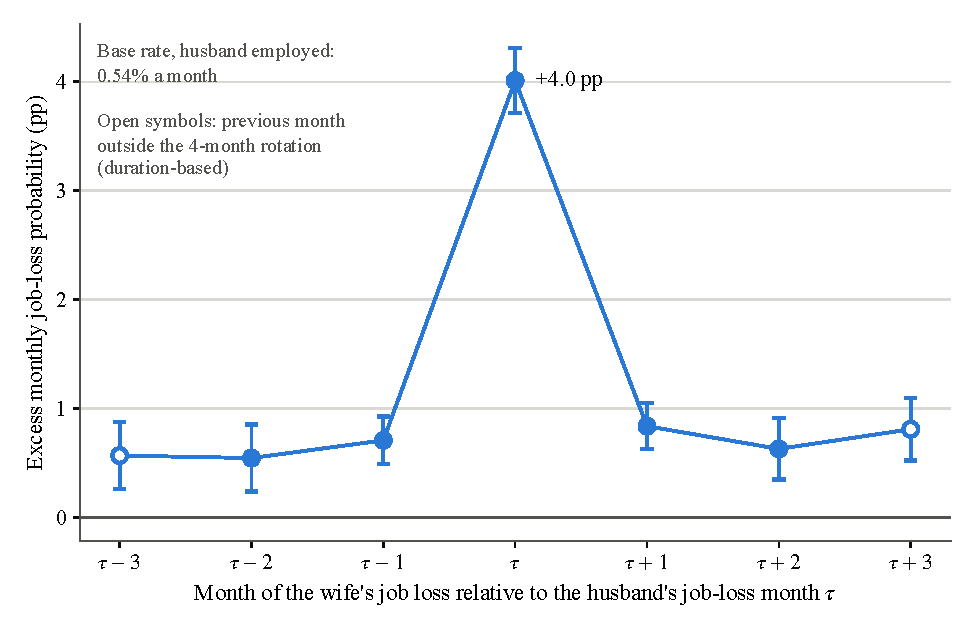
\includegraphics[width=0.85\textwidth]{fig_cps_monthly_hazard.pdf}}%
{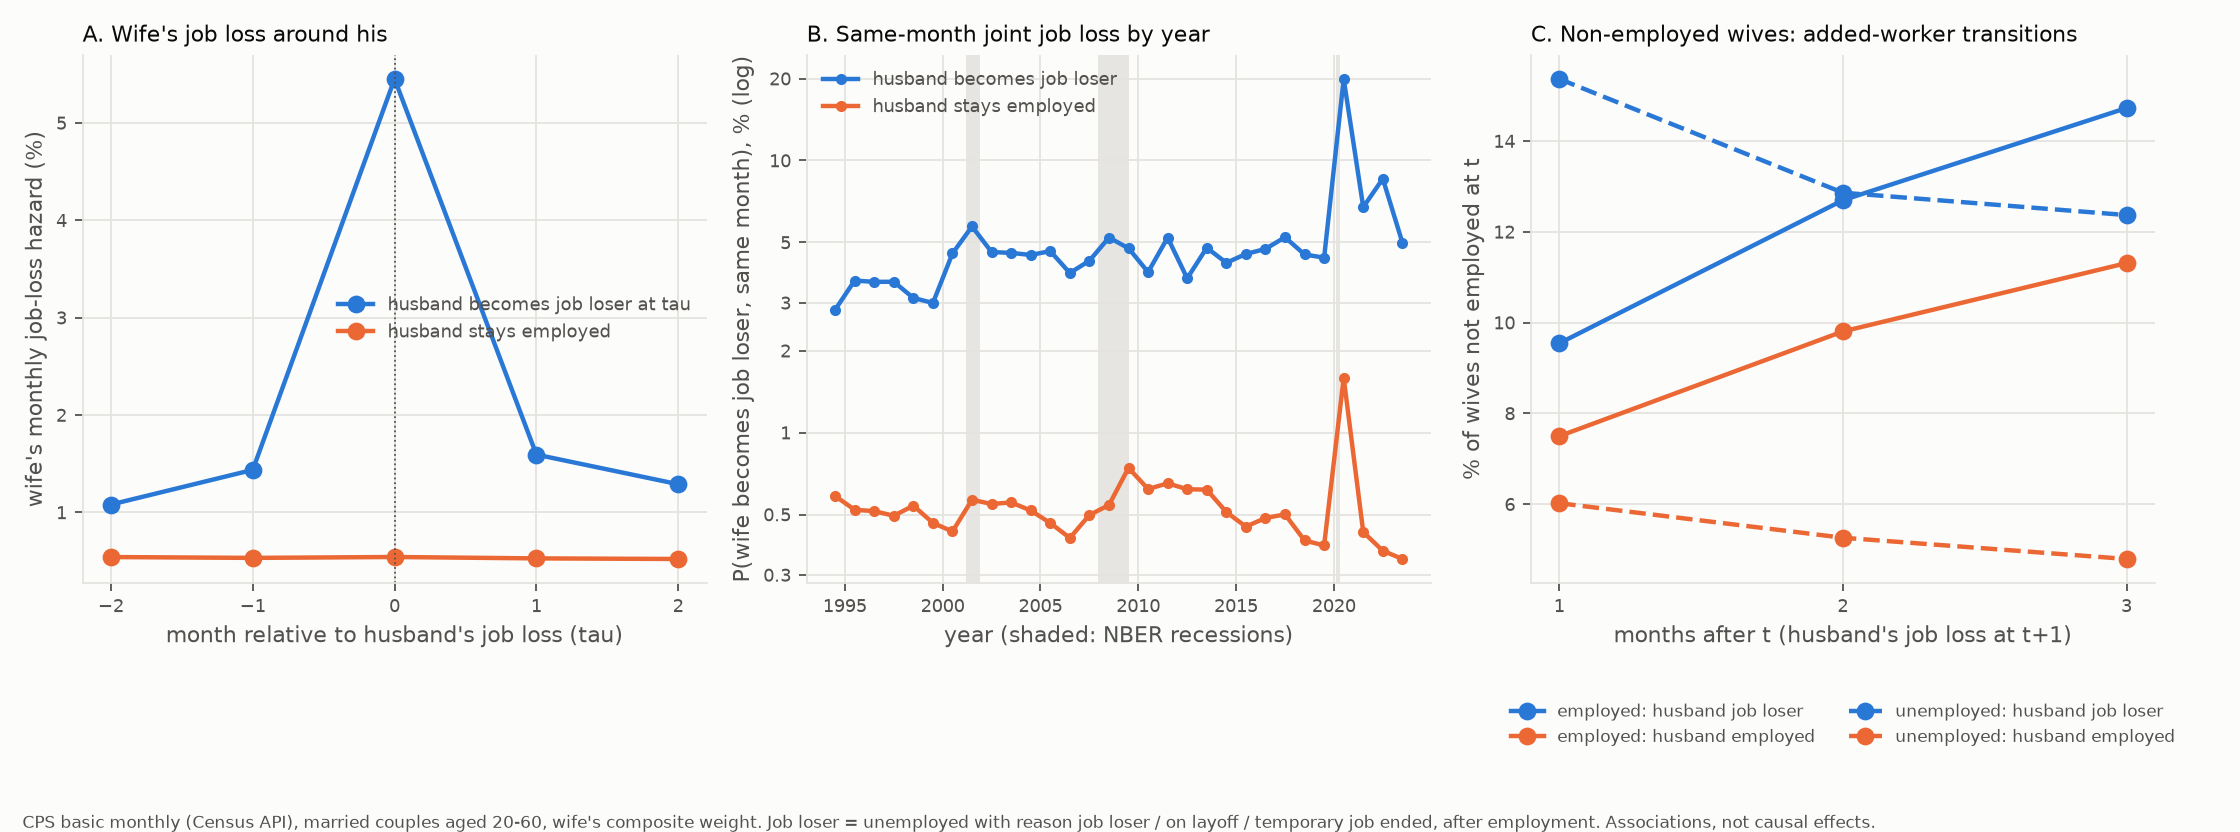
\includegraphics[width=\textwidth]{cps_joint_job_loss.png}}
\caption{The wife's monthly job-loss hazard around her husband's job loss (CPS)}\label{fig:cps_hazard}
\begin{minipage}{0.95\textwidth}\footnotesize Excess probability that the wife loses her job in month $\tau$ relative to
the month in which her husband loses his ($\tau=0$), among couples in which both spouses work; linear probability
models with state $\times$ month fixed effects, 95\% confidence intervals clustered by household. CPS basic monthly
files 1994--2023. At $\tau=\pm3$ the month lies outside the four-month rotation, and a job loss is counted as
unemployment for a job-loss reason lasting four weeks or less (open symbols); the same rule gives 0.041 at $\tau=0$,
against 0.040 from the monthly flows. Code: \texttt{IGE/30.CPSJointJobLoss.py}, \texttt{IGE/37.CPSJointLossChecks.py}.\end{minipage}
\end{figure}

Shared workplaces carry the excess. When the spouses work in the same major industry it rises by 14.8 points
(0.148$^{***}$), and in the same detailed industry 23.0\% of wives lose their job in the month their husband does. The
excess is the same in both races (Black 0.044$^{***}$ on a base of 0.60\%, White 0.038$^{***}$ on 0.54\%; difference
0.006, $p=0.309$), and it does not depend on whether the couple has young children.

\subsection{Reporting, recall layoffs and the season}

Three features of the CPS could produce a joint job loss that is not one: one household member usually reports for
both spouses, a third of the husbands' job losses are temporary layoffs, and some jobs end with the season or the
school year. None of them accounts for the fact (Appendix~\ref{app:robust}, Table~\ref{tab:cps_checks}). The excess is
3.8 points whether the wife or the husband reports the other's job loss. Temporary layoffs account for about a third of
it: without them the excess is 2.7 points, on a base of 0.23\% for permanent job losses. A joint permanent job
loss---both spouses still unemployed two months later, outside temporary layoffs, the summer and the pandemic---is 13
times as likely in the month the husband loses his job as in other months (1.6 points on a base of 0.17\%). Couples who
share a detailed industry, occupation and class of worker, the closest the CPS comes to a common employer, account for
about a third of the excess, so a shared employer plausibly carries a third to a half of it.

\subsection{Displacements with each spouse's own reason}

The PSID measures the same fact with each spouse's own report of why a job ended, over the years around the husband's
displacement (Table~\ref{tab:joint_job_loss}). In the main sample, in which both a window around the event and a
placebo window before it are observed, the husband's displacement raises the probability that his wife is displaced in
the three years around it by 5.2 percentage points (0.052$^{***}$), from a base of 5.8\%, and in the placebo window four
to two years before it by 2.1 points (0.021$^{*}$, $p=0.093$); with couple fixed effects the difference is 3.1 points
(0.031$^{*}$, $p=0.077$). Wives of men who will be displaced four to six years later are already more often displaced in
the placebo window (0.033$^{**}$, $p=0.012$). Part of the excess is therefore a permanent trait of couples who share
risk and part is contemporaneous: stacking both windows, the permanent couple component is 2.0 points (0.020$^{**}$,
$p=0.012$) and the contemporaneous component 3.3 points (0.033$^{**}$, $p=0.036$). In the sample in which only the window around the event is
required the excess is 8.3 points (0.083$^{***}$), and the event study with couple and calendar-year fixed effects puts
the excess in the year of the husband's job loss (3.6 points) and the year after (2.4 points). The CPS, which measures
timing to the month, shows that the contemporaneous part dominates: the leads are 0.6--0.7 points against a
4.0-point spike.\footnote{Couple and calendar-year fixed effects, reference years $-4$ and $-3$; the estimate is already
elevated in year $-2$ (1.8 points, $p=0.07$), consistent with the spouses' reports dating the same events a year apart,
with shocks reaching the workplace first, or with the permanent component. The excess rises across periods, from 0.027
(not significant) in 1984--89 to 0.073$^{***}$ in 1990--99 and 0.095$^{***}$ in 2000--21 (difference 0.069$^{**}$). The rise
is not dating, since more than 97\% of both spouses' reports carry an end year in every period, and not sorting, since
the share of displaced couples in the same sector falls from 0.20 to 0.13; the 1984--89 estimate rests on 175 displaced
husbands. Code: \texttt{IGE/38.PSIDJointLossChecks.py}. Code:
\texttt{IGE/25.JointJobLoss.py}.}

\begin{table}[htbp]\centering\small
\caption{The wife's own job loss around her husband's displacement}\label{tab:joint_job_loss}
\resizebox{\textwidth}{!}{%
\begin{tabular}{lccccccc}
\toprule
 & \begin{tabular}[b]{@{}c@{}}(1) Wife displaced\\$ev-1$ to $ev+1$\end{tabular} & \begin{tabular}[b]{@{}c@{}}(2) Wife displaced\\$ev-4$ to $ev-2$\end{tabular} & \begin{tabular}[b]{@{}c@{}}(3) Wife displaced\\difference\end{tabular} & \begin{tabular}[b]{@{}c@{}}(4) Any job end\\$ev-1$ to $ev+1$\end{tabular} & \begin{tabular}[b]{@{}c@{}}(5) Any job end\\difference\end{tabular} & \begin{tabular}[b]{@{}c@{}}(6) Employer closed\\$ev-1$ to $ev+1$\end{tabular} & \begin{tabular}[b]{@{}c@{}}(7) Employer closed\\difference\end{tabular} \\
\midrule
\multicolumn{8}{l}{\textit{A. All couples}} \\
Husband displaced in $ev$ & $0.052^{***}$ & $0.021^{*}$ & $0.031^{*}$ & $0.122^{***}$ & $0.073^{**}$ & $0.015^{*}$ & $0.008$ \\
 & (0.014) & (0.013) & (0.017) & (0.022) & (0.029) & (0.009) & (0.011) \\
Husband displaced in $ev+4$ to $ev+6$ & $0.007$ & $0.033^{**}$ & $-0.026$ & $0.051^{**}$ & $-0.016$ & $-0.010^{**}$ & $-0.008$ \\
 & (0.012) & (0.013) & (0.016) & (0.022) & (0.023) & (0.005) & (0.007) \\
Husband displaced in $ev$, window-only sample & $0.083^{***}$ &  &  & $0.170^{***}$ &  & $0.019^{**}$ &  \\
 & (0.013) &  &  & (0.018) &  & (0.008) &  \\
Event study, sum of years $-1$ to $+1$ & $0.081^{***}$ &  &  & $0.153^{***}$ &  & $0.021$ &  \\
 & (0.022) &  &  & (0.043) &  & (0.013) &  \\
Control mean & 0.058 & 0.056 & 0.001 & 0.289 & -0.012 & 0.021 & 0.001 \\
Couples & 21,584 & 21,584 & 21,584 & 21,584 & 21,584 & 21,584 & 21,584 \\
\multicolumn{8}{l}{\textit{B. Black couples}} \\
Husband displaced in $ev$ & $0.081^{***}$ & $0.022$ & $0.059^{*}$ & $0.111^{***}$ & $0.090^{*}$ & $0.015$ & $0.010$ \\
 & (0.029) & (0.026) & (0.034) & (0.040) & (0.050) & (0.016) & (0.019) \\
Husband displaced in $ev+4$ to $ev+6$ & $-0.008$ & $0.051^{*}$ & $-0.059$ & $0.033$ & $-0.060$ & $-0.020^{**}$ & $-0.020$ \\
 & (0.025) & (0.029) & (0.039) & (0.045) & (0.047) & (0.009) & (0.017) \\
Husband displaced in $ev$, window-only sample & $0.088^{***}$ &  &  & $0.151^{***}$ &  & $0.017$ &  \\
 & (0.024) &  &  & (0.031) &  & (0.012) &  \\
Event study, sum of years $-1$ to $+1$ & $0.140^{***}$ &  &  & $0.166^{**}$ &  & $0.018$ &  \\
 & (0.036) &  &  & (0.069) &  & (0.021) &  \\
Control mean & 0.078 & 0.080 & -0.001 & 0.291 & -0.013 & 0.027 & 0.000 \\
Couples & 4,920 & 4,920 & 4,920 & 4,920 & 4,920 & 4,920 & 4,920 \\
\multicolumn{8}{l}{\textit{C. White couples}} \\
Husband displaced in $ev$ & $0.036^{**}$ & $0.017$ & $0.019$ & $0.125^{***}$ & $0.065^{*}$ & $0.015$ & $0.008$ \\
 & (0.016) & (0.014) & (0.020) & (0.027) & (0.034) & (0.010) & (0.013) \\
Husband displaced in $ev+4$ to $ev+6$ & $0.010$ & $0.022$ & $-0.012$ & $0.060^{**}$ & $0.003$ & $-0.006$ & $-0.003$ \\
 & (0.013) & (0.014) & (0.017) & (0.025) & (0.026) & (0.006) & (0.006) \\
Husband displaced in $ev$, window-only sample & $0.077^{***}$ &  &  & $0.176^{***}$ &  & $0.020^{**}$ &  \\
 & (0.016) &  &  & (0.023) &  & (0.010) &  \\
Event study, sum of years $-1$ to $+1$ & $0.047^{*}$ &  &  & $0.142^{***}$ &  & $0.023$ &  \\
 & (0.028) &  &  & (0.055) &  & (0.017) &  \\
Control mean & 0.052 & 0.050 & 0.002 & 0.289 & -0.012 & 0.020 & 0.001 \\
Couples & 16,664 & 16,664 & 16,664 & 16,664 & 16,664 & 16,664 & 16,664 \\
\multicolumn{8}{l}{\textit{D. Black $-$ White (pooled, interactions)}} \\
Husband displaced in $ev$ $\times$ Black & $0.042$ & $0.004$ & $0.038$ & $-0.007$ & $0.032$ & $-0.002$ & $-0.001$ \\
 & (0.033) & (0.029) & (0.039) & (0.048) & (0.061) & (0.019) & (0.023) \\
\bottomrule
\end{tabular}}
\begin{minipage}{0.95\textwidth}\footnotesize Unit: a father $\times$ event year $ev$ with his wife employed at baseline; the treated are fathers first displaced (plant closed or moved, laid off or fired) in $ev$, the controls fathers not displaced up to $ev+6$, and the future placebo fathers first displaced in $ev+4$ to $ev+6$. Outcomes: the wife's own report that a job of hers ended because she was laid off or fired or her employer closed (displaced), for any reason (any job end), or because her employer closed, dated in the window of the column; ``difference'' is the window $ev-1$ to $ev+1$ minus the window $ev-4$ to $ev-2$, which removes any permanent difference in the wife's job stability. Event years 1987--2021, both windows observed. OLS with event-year fixed effects. ``Window-only sample'': the same regression among all couples whose window $ev-1$ to $ev+1$ is observed (the placebo window need not be; 26,024 couples, 738 displaced). ``Event study'': sum of the coefficients for years $-1$, $0$ and $+1$ from a regression of the wife's annual job-loss indicator in years $-4$ to $+4$ on displaced $\times$ year dummies with couple and calendar-year fixed effects, reference years $-4$ and $-3$ (event years 1987--2018; figure \texttt{output/joint\_job\_loss\_es.png}). PSID SRC and SEO, unweighted. Standard errors clustered by 1968 family in parentheses. *** $p<0.01$, ** $p<0.05$, * $p<0.1$. Source: \texttt{IGE/25.JointJobLoss.py}.\end{minipage}
\end{table}

\begin{table}[htbp]\centering\small
\caption{Joint job loss: closures, shared labor markets and pre-trends}\label{tab:joint_job_loss_id}
\resizebox{\textwidth}{!}{%
\begin{tabular}{lccccccccc}
\toprule
 & \begin{tabular}[b]{@{}c@{}}(1) Closures\\only\end{tabular} & \begin{tabular}[b]{@{}c@{}}(2) Closures only:\\her employer\\closed\end{tabular} & \begin{tabular}[b]{@{}c@{}}(3) Layoffs\\only\end{tabular} & \begin{tabular}[b]{@{}c@{}}(4) Same\\sector\end{tabular} & \begin{tabular}[b]{@{}c@{}}(5) Same 3-digit\\industry\end{tabular} & \begin{tabular}[b]{@{}c@{}}(6) Same\\occupation\end{tabular} & \begin{tabular}[b]{@{}c@{}}(7) State\\unemployment\end{tabular} & \begin{tabular}[b]{@{}c@{}}(8) Pre-trend\\controls\end{tabular} & \begin{tabular}[b]{@{}c@{}}(9) No self-\\employed\end{tabular} \\
\midrule
\multicolumn{10}{l}{\textit{A. All couples}} \\
Husband displaced & $0.068^{**}$ & $0.054^{**}$ & $0.044^{***}$ & $0.023^{*}$ & $0.030^{**}$ & $0.039^{**}$ & $0.053^{***}$ & $0.048^{***}$ & $0.038^{**}$ \\
 & (0.027) & (0.021) & (0.016) & (0.014) & (0.014) & (0.015) & (0.014) & (0.014) & (0.016) \\
Displaced $\times$ wife in his sector &  &  &  & $0.203^{***}$ &  &  &  &  &  \\
 &  &  &  & (0.055) &  &  &  &  &  \\
Wife in his sector &  &  &  & $-0.016^{***}$ &  &  &  &  &  \\
 &  &  &  & (0.005) &  &  &  &  &  \\
Displaced $\times$ same 3-digit industry &  &  &  &  & $0.282^{***}$ &  &  &  &  \\
 &  &  &  &  & (0.078) &  &  &  &  \\
Same 3-digit industry &  &  &  &  & $-0.032^{***}$ &  &  &  &  \\
 &  &  &  &  & (0.005) &  &  &  &  \\
Displaced $\times$ same occupation group &  &  &  &  &  & $0.083^{**}$ &  &  &  \\
 &  &  &  &  &  & (0.042) &  &  &  \\
Same occupation group &  &  &  &  &  & $-0.015^{***}$ &  &  &  \\
 &  &  &  &  &  & (0.005) &  &  &  \\
Displaced $\times$ $\Delta$ state unemployment (s.d.) &  &  &  &  &  &  & $0.020$ &  &  \\
 &  &  &  &  &  &  & (0.017) &  &  \\
$\Delta$ state unemployment (s.d.) &  &  &  &  &  &  & $0.004$ &  &  \\
 &  &  &  &  &  &  & (0.005) &  &  \\
Wife displaced in $ev-4$ to $ev-2$ &  &  &  &  &  &  &  & $0.086^{***}$ &  \\
 &  &  &  &  &  &  &  & (0.014) &  \\
Control mean & 0.058 & 0.021 & 0.058 & 0.057 & 0.057 & 0.057 & 0.057 & 0.058 & 0.060 \\
Couples & 20,394 & 20,394 & 20,566 & 20,401 & 20,567 & 20,198 & 20,614 & 20,723 & 15,106 \\
\multicolumn{10}{l}{\textit{B. Black couples}} \\
Husband displaced & $0.110^{*}$ & $0.066$ & $0.067^{**}$ & $0.045$ & $0.064^{**}$ & $0.058^{*}$ & $0.081^{***}$ & $0.078^{***}$ & $0.059^{*}$ \\
 & (0.058) & (0.044) & (0.033) & (0.030) & (0.029) & (0.030) & (0.029) & (0.028) & (0.031) \\
Displaced $\times$ wife in his sector &  &  &  & $0.196^{**}$ &  &  &  &  &  \\
 &  &  &  & (0.089) &  &  &  &  &  \\
Displaced $\times$ same 3-digit industry &  &  &  &  & $0.201$ &  &  &  &  \\
 &  &  &  &  & (0.129) &  &  &  &  \\
Displaced $\times$ same occupation group &  &  &  &  &  & $0.147^{*}$ &  &  &  \\
 &  &  &  &  &  & (0.087) &  &  &  \\
Displaced $\times$ $\Delta$ state unemployment (s.d.) &  &  &  &  &  &  & $0.002$ &  &  \\
 &  &  &  &  &  &  & (0.038) &  &  \\
Wife displaced in $ev-4$ to $ev-2$ &  &  &  &  &  &  &  & $0.058^{**}$ &  \\
 &  &  &  &  &  &  &  & (0.024) &  \\
Control mean & 0.078 & 0.027 & 0.078 & 0.077 & 0.078 & 0.077 & 0.079 & 0.078 & 0.082 \\
Couples & 4,557 & 4,557 & 4,627 & 4,576 & 4,605 & 4,489 & 4,655 & 4,671 & 3,907 \\
\multicolumn{10}{l}{\textit{C. White couples}} \\
Husband displaced & $0.051^{*}$ & $0.048^{**}$ & $0.028$ & $0.012$ & $0.011$ & $0.028$ & $0.037^{**}$ & $0.033^{**}$ & $0.023$ \\
 & (0.029) & (0.024) & (0.018) & (0.015) & (0.015) & (0.017) & (0.016) & (0.016) & (0.018) \\
Displaced $\times$ wife in his sector &  &  &  & $0.190^{***}$ &  &  &  &  &  \\
 &  &  &  & (0.070) &  &  &  &  &  \\
Displaced $\times$ same 3-digit industry &  &  &  &  & $0.318^{***}$ &  &  &  &  \\
 &  &  &  &  & (0.097) &  &  &  &  \\
Displaced $\times$ same occupation group &  &  &  &  &  & $0.047$ &  &  &  \\
 &  &  &  &  &  & (0.044) &  &  &  \\
Displaced $\times$ $\Delta$ state unemployment (s.d.) &  &  &  &  &  &  & $0.028$ &  &  \\
 &  &  &  &  &  &  & (0.019) &  &  \\
Wife displaced in $ev-4$ to $ev-2$ &  &  &  &  &  &  &  & $0.093^{***}$ &  \\
 &  &  &  &  &  &  &  & (0.017) &  \\
Control mean & 0.052 & 0.020 & 0.052 & 0.051 & 0.051 & 0.051 & 0.051 & 0.052 & 0.053 \\
Couples & 15,837 & 15,837 & 15,939 & 15,825 & 15,962 & 15,709 & 15,959 & 16,052 & 11,199 \\
\bottomrule
\end{tabular}}
\begin{minipage}{0.95\textwidth}\footnotesize Sample of Table~\ref{tab:joint_job_loss} without the future placebo; outcome: the wife displaced in $ev-1$ to $ev+1$ (column 2: her employer closed). Columns 1--2 keep displaced husbands whose job loss was a plant closure, column 3 those laid off or fired. Columns 4--6 interact the displacement with the spouses working in the same of 16 sectors, the same 3-digit Census industry, or the same of 8 major occupation groups (husband: latest interview in $ev-3$ to $ev$; wife: $ev-6$ to $ev$). Column 7: change in the state unemployment rate in $ev$ (LAUS), in standard deviations among the displaced. Column 8 controls for the husband's hours and labor income at $ev-2$ ($ev-3$ in biennial years) and their change over the two years before, the wife's hours likewise, and her displacement in $ev-4$ to $ev-2$. Column 9 drops couples in which either spouse was self-employed at an interview in $ev-3$ to $ev$. Main effects of the match variables are included in every panel (shown in panel A). OLS with event-year fixed effects; standard errors clustered by 1968 family. *** $p<0.01$, ** $p<0.05$, * $p<0.1$. Source: \texttt{IGE/25.JointJobLoss.py}.\end{minipage}
\end{table}

\begin{table}[htbp]\centering\small
\caption{How often both spouses lose their jobs}\label{tab:joint_job_loss_magnitudes}
\resizebox{\textwidth}{!}{%
\begin{tabular}{lccccc}
\toprule
 & \begin{tabular}[b]{@{}c@{}}(1) P(she is displaced\\$\mid$ he is)\end{tabular} & \begin{tabular}[b]{@{}c@{}}(2) P(she is displaced\\$\mid$ he is not)\end{tabular} & \begin{tabular}[b]{@{}c@{}}(3) Difference\\\end{tabular} & \begin{tabular}[b]{@{}c@{}}(4) Phi\\coefficient\end{tabular} & \begin{tabular}[b]{@{}c@{}}(5) Tetrachoric\\correlation\end{tabular} \\
\midrule
\multicolumn{6}{l}{\textit{A. Same year (interval)}} \\
All couple-years & 0.102 & 0.039 & $0.063^{***}$ & $0.070^{***}$ & $0.237^{***}$ \\
 & & & (0.005) & (0.006) & (0.016) \\
Black & 0.105 & 0.049 & $0.056^{***}$ & $0.064^{***}$ & $0.201^{***}$ \\
 & & & (0.009) & (0.010) & (0.025) \\
White & 0.100 & 0.036 & $0.064^{***}$ & $0.071^{***}$ & $0.248^{***}$ \\
 & & & (0.006) & (0.007) & (0.018) \\
Same sector & 0.211 & 0.028 & $0.183^{***}$ & $0.186^{***}$ & $0.504^{***}$ \\
 & & & (0.022) & (0.020) & (0.032) \\
Different sector & 0.076 & 0.035 & $0.041^{***}$ & $0.047^{***}$ & $0.182^{***}$ \\
 & & & (0.006) & (0.006) & (0.020) \\
Youngest child 0--5 & 0.105 & 0.040 & $0.065^{***}$ & $0.077^{***}$ & $0.245^{***}$ \\
 & & & (0.009) & (0.010) & (0.026) \\
Youngest child 6--17 & 0.091 & 0.041 & $0.050^{***}$ & $0.055^{***}$ & $0.197^{***}$ \\
 & & & (0.009) & (0.010) & (0.028) \\
No child under 18 & 0.108 & 0.037 & $0.072^{***}$ & $0.076^{***}$ & $0.263^{***}$ \\
 & & & (0.009) & (0.010) & (0.025) \\
Annual survey years (to 1996) & 0.090 & 0.039 & $0.051^{***}$ & $0.055^{***}$ & $0.200^{***}$ \\
 & & & (0.007) & (0.008) & (0.023) \\
\multicolumn{6}{l}{\textit{B. Within one year}} \\
All couple-years & 0.181 & 0.091 & $0.090^{***}$ & $0.067^{***}$ & $0.201^{***}$ \\
 & & & (0.008) & (0.006) & (0.015) \\
Black & 0.183 & 0.113 & $0.070^{***}$ & $0.055^{***}$ & $0.151^{***}$ \\
 & & & (0.015) & (0.012) & (0.030) \\
White & 0.180 & 0.084 & $0.096^{***}$ & $0.071^{***}$ & $0.216^{***}$ \\
 & & & (0.009) & (0.006) & (0.016) \\
Same sector & 0.275 & 0.064 & $0.211^{***}$ & $0.151^{***}$ & $0.415^{***}$ \\
 & & & (0.024) & (0.017) & (0.031) \\
Different sector & 0.148 & 0.080 & $0.068^{***}$ & $0.052^{***}$ & $0.168^{***}$ \\
 & & & (0.009) & (0.006) & (0.017) \\
Youngest child 0--5 & 0.206 & 0.097 & $0.109^{***}$ & $0.087^{***}$ & $0.235^{***}$ \\
 & & & (0.015) & (0.012) & (0.026) \\
Youngest child 6--17 & 0.164 & 0.095 & $0.069^{***}$ & $0.051^{***}$ & $0.156^{***}$ \\
 & & & (0.013) & (0.009) & (0.025) \\
No child under 18 & 0.174 & 0.084 & $0.090^{***}$ & $0.065^{***}$ & $0.205^{***}$ \\
 & & & (0.013) & (0.010) & (0.025) \\
Annual survey years (to 1996) & 0.190 & 0.104 & $0.086^{***}$ & $0.059^{***}$ & $0.178^{***}$ \\
 & & & (0.012) & (0.008) & (0.021) \\
\bottomrule
\end{tabular}}
\begin{minipage}{0.95\textwidth}\footnotesize Couple-years: consecutive interviews of the same married couple, both spouses with positive hours in the earlier year, intervals ending 1984--2022 (one year to 1996, two years in the biennial survey; the last row keeps one-year intervals). Panel A: both spouses displaced (closure, layoff or firing) in the same interval; panel B: her displacement within one year either side of the interval. Column 3: OLS of her displacement on his, standard error clustered by 1968 family; columns 4--5: standard errors from 200 bootstrap draws of 1968 families. *** $p<0.01$, ** $p<0.05$, * $p<0.1$. Source: \texttt{IGE/25.JointJobLoss.py}.\end{minipage}
\end{table}


\begin{figure}[htbp]\centering
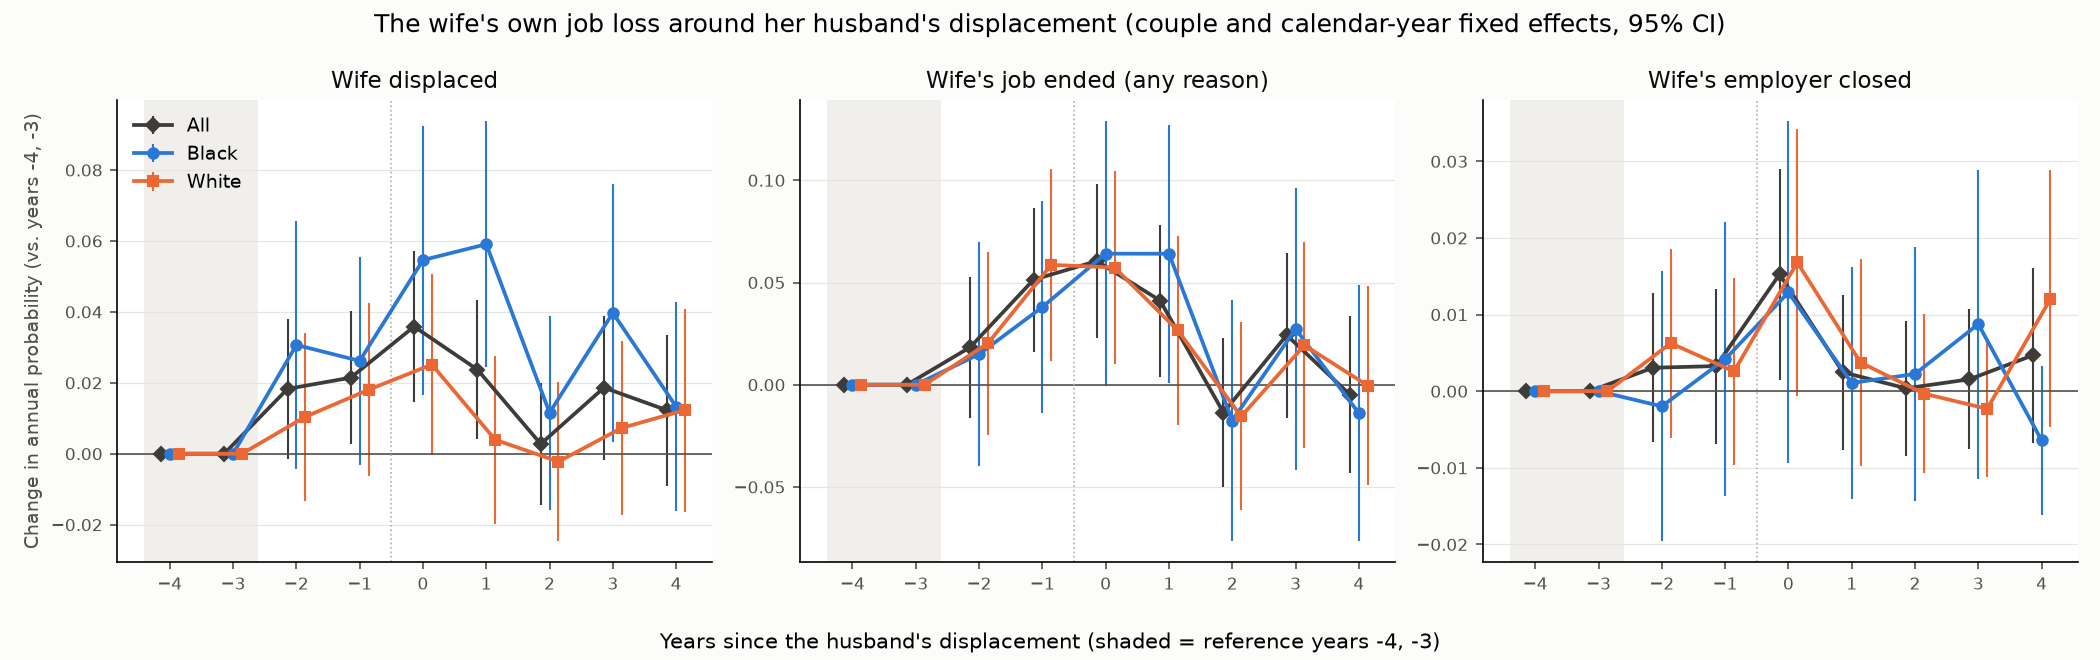
\includegraphics[width=\textwidth]{joint_job_loss_es.png}
\caption{The wife's own job loss around her husband's displacement (PSID)}\label{fig:joint_job_loss}
\begin{minipage}{0.95\textwidth}\footnotesize Event study of the wife's displacement and of her employer's closure,
by year relative to the husband's displacement (reference years $-4$ and $-3$), with 95\% confidence intervals; wives
working at baseline, couple and calendar-year fixed effects. Code: \texttt{IGE/25.JointJobLoss.py}.\end{minipage}
\end{figure}

The channels are the same as in the CPS. When the husband's job loss is a plant closure, the wife's risk of
displacement rises by 6.8 points and the probability that her own employer closes by 5.4 points. Where the spouses work
in the same one of 16 sectors (15\% of couples), the husband's displacement raises her risk by a further 20 points, and
in the same three-digit industry (8\% of couples), the closest the public PSID comes to a common employer, by 28 points.
The change in the state unemployment rate does not moderate it. Controlling for both spouses' hours and earnings before
the job loss leaves an excess of 4.8 points.

\subsection{Two more data sets: the Displaced Worker Supplement and the SIPP}

The CPS Displaced Worker Supplement (1984--2024) records each adult's displacements with the reason and the year in
417,269 couples. A wife was displaced in the same calendar year as her husband in 4.7\% of couples in which he was
displaced and in 1.1\% of the others (an excess of 3.3 points, 0.033$^{***}$), joint plant closings within the same year
are almost ten times as frequent as independent closings would imply, and 68\% of same-year joint closings are in the
same detailed industry. The Survey of Income and Program Participation (SIPP; 2004, 2008 and 2014 panels; 50,692
couples) follows both spouses month by month for up to five years with each job's reason for ending. A wife has an
involuntary separation in the month of her husband's 7.7 times as often as otherwise (an excess of 2.7 points,
0.027$^{***}$), 13 times with a definition close to the CPS one; the excess holds for couples in which both spouses
report for themselves (0.019$^{***}$) and rises by 22 points when the spouses share a detailed industry. In both data
sets the tetrachoric or relative measures match the PSID and the CPS. The excess is the same for Black and White
couples in the CPS and the Displaced Worker Supplement; in the SIPP the same-month excess is smaller for Black couples,
on six joint events, while the twelve-month excess is similar (Appendix~\ref{app:robust}).

\paragraph{By age.} The joint job loss is not a feature of young couples. Outside temporary layoffs, the wife's excess
risk of losing her job in the month her husband loses his is 2.8 percentage points when she is 26--35, 2.4 at 36--45, 2.4
at 46--55 and 2.7 at 56--62 (oldest minus youngest $-0.05$, $p=0.94$); including temporary layoffs it rises with age, from
3.6 to 5.0 points. In the same panel the added worker effect of \citet{bacher2025joint}---the response of a
non-participating spouse to the working spouse's job loss---is 5.6 points (their estimate: 5.55) and declines with age,
from 6.4 points at 26--35 and 7.2 at 36--45 to 1.2 at 56--62, as in their data.\footnote{Couples of a working and a
non-participating spouse, primary earner's transition from employment to unemployment against continued employment,
classification-error adjustment of \citet{bacher2025joint}, 1994--2020; oldest minus youngest $-5.13^{***}$ (s.e.\ 1.03).
Joint job loss: state $\times$ month fixed effects; the same-month joint rate is 6.1 times its value under independence
at 20--25 and 10.7 times at 56--62. Code: \texttt{IGE/50.CPSAddedWorkerByAge.py} (\texttt{output/cps\_awe\_by\_age.md}).}
Older couples, whose non-working spouse barely enters the labor force, remain exposed to the loss of both earners
(Figure~\ref{fig:age_awe_jointloss}).

\begin{figure}[htbp]\centering
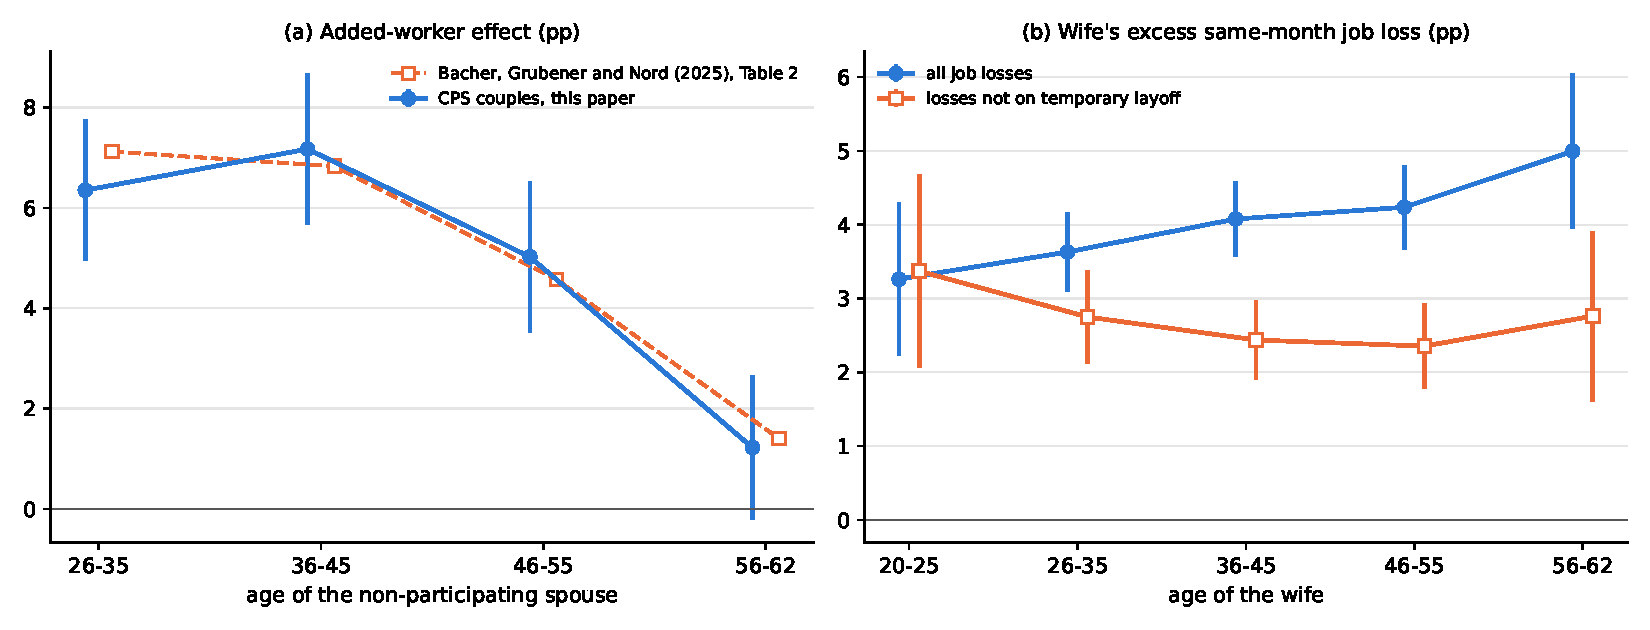
\includegraphics[width=\textwidth]{fig_cps_age_awe_jointloss.pdf}
\caption{The added worker effect and the joint job loss by age (CPS)}\label{fig:age_awe_jointloss}
\begin{minipage}{0.95\textwidth}\footnotesize (a) Added worker effect: the probability that a non-participating spouse
enters the labor force when the working spouse moves from employment to unemployment, minus the same probability when
the working spouse stays employed, by the non-participating spouse's age, with the classification-error adjustment of
\citet{bacher2025joint}, 1994--2020; open squares: their Table~2 (their oldest group is 56--65). Oldest minus youngest
$-5.13^{***}$ (s.e.\ 1.03, $p<0.001$). (b) Excess probability that the working wife loses her job in the month her
husband loses his, by her age; linear probability models with state $\times$ month fixed effects, 1994--2023; open
squares exclude losses on temporary layoff of either spouse. Oldest minus 26--35: all losses 1.45$^{**}$ points (s.e.\
0.63, $p=0.021$; equality across all ages $p=0.11$), losses not on temporary layoff $-0.05$ (s.e.\ 0.68, $p=0.94$;
equality across all ages $p=0.77$). 95\% confidence
intervals clustered by household. Code: \texttt{50.CPSAddedWorkerByAge.py} (\texttt{output/cps\_awe\_by\_age.csv}).
\end{minipage}
\end{figure}

\subsection{Magnitudes for the model}

Table~\ref{tab:joint_job_loss_magnitudes} expresses the result as joint probabilities. Among working couples, the wife
is displaced in 10.2\% of the years in which her husband is and in 3.9\% of the years in which he is not, a tetrachoric
correlation of job loss within the couple of 0.24, which rises to 0.50 when the spouses share a sector. These are the
moments the model targets: a common component of the spouses' displacement risk, larger for couples who share a sector,
on top of a permanent component of couples who share risk.

The joint loss is small in the household's average income loss. A wife's displacement costs her about \$4,600 a year in
labor income; averaged over all displaced families, the joint losses lower wives' earnings by about \$260 a year, about
a fifth of the amount by which family income falls beyond the husband's own earnings and about 2\% of the family's
income loss. It does not explain why wives insure little on average. Its importance lies in the state and the
subgroup in which it occurs: in the month of the shock, when the household's income falls most, and among couples who
share a workplace, where one job loss in five takes both earners. That is where insurance is valued most, and it is
absent from models of family insurance.

\section{What the Household Loses and What It Does}\label{sec:household}

\subsection{The father's earnings and the family's income}

Table~\ref{tab:displacement_family} reports the mean effects of the father's displacement over years 1 to 3 after the
job loss, and Figure~\ref{fig:displacement_es} the effects year by year. The job loss is a large and lasting shock.
His hours fall by about 300 in the year of the job loss and recover within four to five years, but his labor income
stays about \$6,000--7,000 a year lower six years later. Over years 1 to 3, his labor income falls by \$4,160 for Black
fathers and \$9,622 for White fathers, about 17\% and 24\% of their pre-displacement labor income. Family income falls by
at least as much (by \$4,832 and \$11,179), so on average none of the loss is made up within the household. Displaced
fathers' earnings were already lower in the year before the job loss (by \$2,821), the dip before displacement that
\citet{jacobson1993earnings} document. It is a fall in hourly earnings, not hours ($-\$1.01$ an hour, while hours
change by $-15$, $p=0.477$), it appears in the reports that carry the year of the job loss rather than in those dated
by assumption, and it is largest before plant closures, as expected of declining employers.\footnote{Code: \texttt{IGE/19.FatherDisplacement.py}, \texttt{IGE/20.PaperDisplacement.py}. Closures-only
versions of every outcome: \texttt{output/father\_displacement.md}, Section 2c.}

\begin{table}[htbp]\centering\small
\caption{The father's displacement and the family}\label{tab:displacement_family}
\resizebox{\textwidth}{!}{%
\begin{tabular}{lcccccccc}
\toprule
 & \begin{tabular}[b]{@{}c@{}}(1) Father's\\hours\end{tabular} & \begin{tabular}[b]{@{}c@{}}(2) Father's\\labor income\end{tabular} & \begin{tabular}[b]{@{}c@{}}(3) Family\\income\end{tabular} & \begin{tabular}[b]{@{}c@{}}(4) Wife's\\hours\end{tabular} & \begin{tabular}[b]{@{}c@{}}(5) Wife\\employed\end{tabular} & \begin{tabular}[b]{@{}c@{}}(6) Still\\with wife\end{tabular} & \begin{tabular}[b]{@{}c@{}}(7) AFDC/TANF\\\end{tabular} & \begin{tabular}[b]{@{}c@{}}(8) Food\\stamps\end{tabular} \\
\midrule
\multicolumn{9}{l}{\textit{A. All fathers}} \\
Displaced, years 1--3 & $-145^{***}$ & $-8,037^{***}$ & $-9,345^{***}$ & $51^{**}$ & $0.008$ & $-0.031^{***}$ & $0.008$ & $0.036^{***}$ \\
 & (22) & (748) & (960) & (23) & (0.013) & (0.008) & (0.005) & (0.010) \\
Displaced / control fathers & \multicolumn{8}{l}{2,417 / 63,669} \\
\multicolumn{9}{l}{\textit{B. Black fathers}} \\
Displaced, years 1--3 & $-146^{***}$ & $-4,160^{***}$ & $-4,832^{***}$ & $40$ & $0.026$ & $-0.045^{***}$ & $0.010$ & $0.042^{**}$ \\
 & (35) & (757) & (1,082) & (38) & (0.019) & (0.015) & (0.009) & (0.019) \\
Displaced / control fathers & \multicolumn{8}{l}{989 / 17,746} \\
\multicolumn{9}{l}{\textit{C. White fathers}} \\
Displaced, years 1--3 & $-130^{***}$ & $-9,622^{***}$ & $-11,179^{***}$ & $59^{**}$ & $-0.002$ & $-0.019^{**}$ & $0.007$ & $0.033^{***}$ \\
 & (28) & (1,071) & (1,353) & (30) & (0.018) & (0.009) & (0.006) & (0.010) \\
Displaced / control fathers & \multicolumn{8}{l}{1,428 / 45,923} \\
\multicolumn{9}{l}{\textit{D. Youngest child aged 0--5}} \\
Displaced, years 1--3 & $-158^{***}$ & $-7,733^{***}$ & $-8,052^{***}$ & $112^{***}$ & $0.041^{**}$ & $-0.030^{***}$ & $0.012^{*}$ & $0.039^{***}$ \\
 & (29) & (976) & (1,127) & (31) & (0.018) & (0.010) & (0.007) & (0.013) \\
\multicolumn{9}{l}{\textit{E. Youngest child aged 6--17}} \\
Displaced, years 1--3 & $-149^{***}$ & $-9,686^{***}$ & $-11,768^{***}$ & $-26$ & $-0.038^{**}$ & $-0.030^{**}$ & $0.002$ & $0.032^{**}$ \\
 & (34) & (1,118) & (1,600) & (36) & (0.018) & (0.012) & (0.008) & (0.014) \\
\bottomrule
\end{tabular}}
\begin{minipage}{0.95\textwidth}\footnotesize Stacked event study of a father's first displacement (plant closed or moved, laid off or fired, from the PSID question on why the last job ended), with clean controls (fathers not displaced up to six years after the event year). Coefficient: mean of the event-time effects at years $+1$ to $+3$, relative to year $-2$. Fathers are male heads with a child aged 0--17 and positive hours at baseline; SRC and SEO samples, Black and White, unweighted. Incomes in 2000 dollars; wife's outcomes for the wife present at baseline. Standard errors clustered by 1968 family. *** $p<0.01$, ** $p<0.05$, * $p<0.1$. Source: \texttt{IGE/19.FatherDisplacement.py}.\end{minipage}
\end{table}


\begin{figure}[htbp]\centering
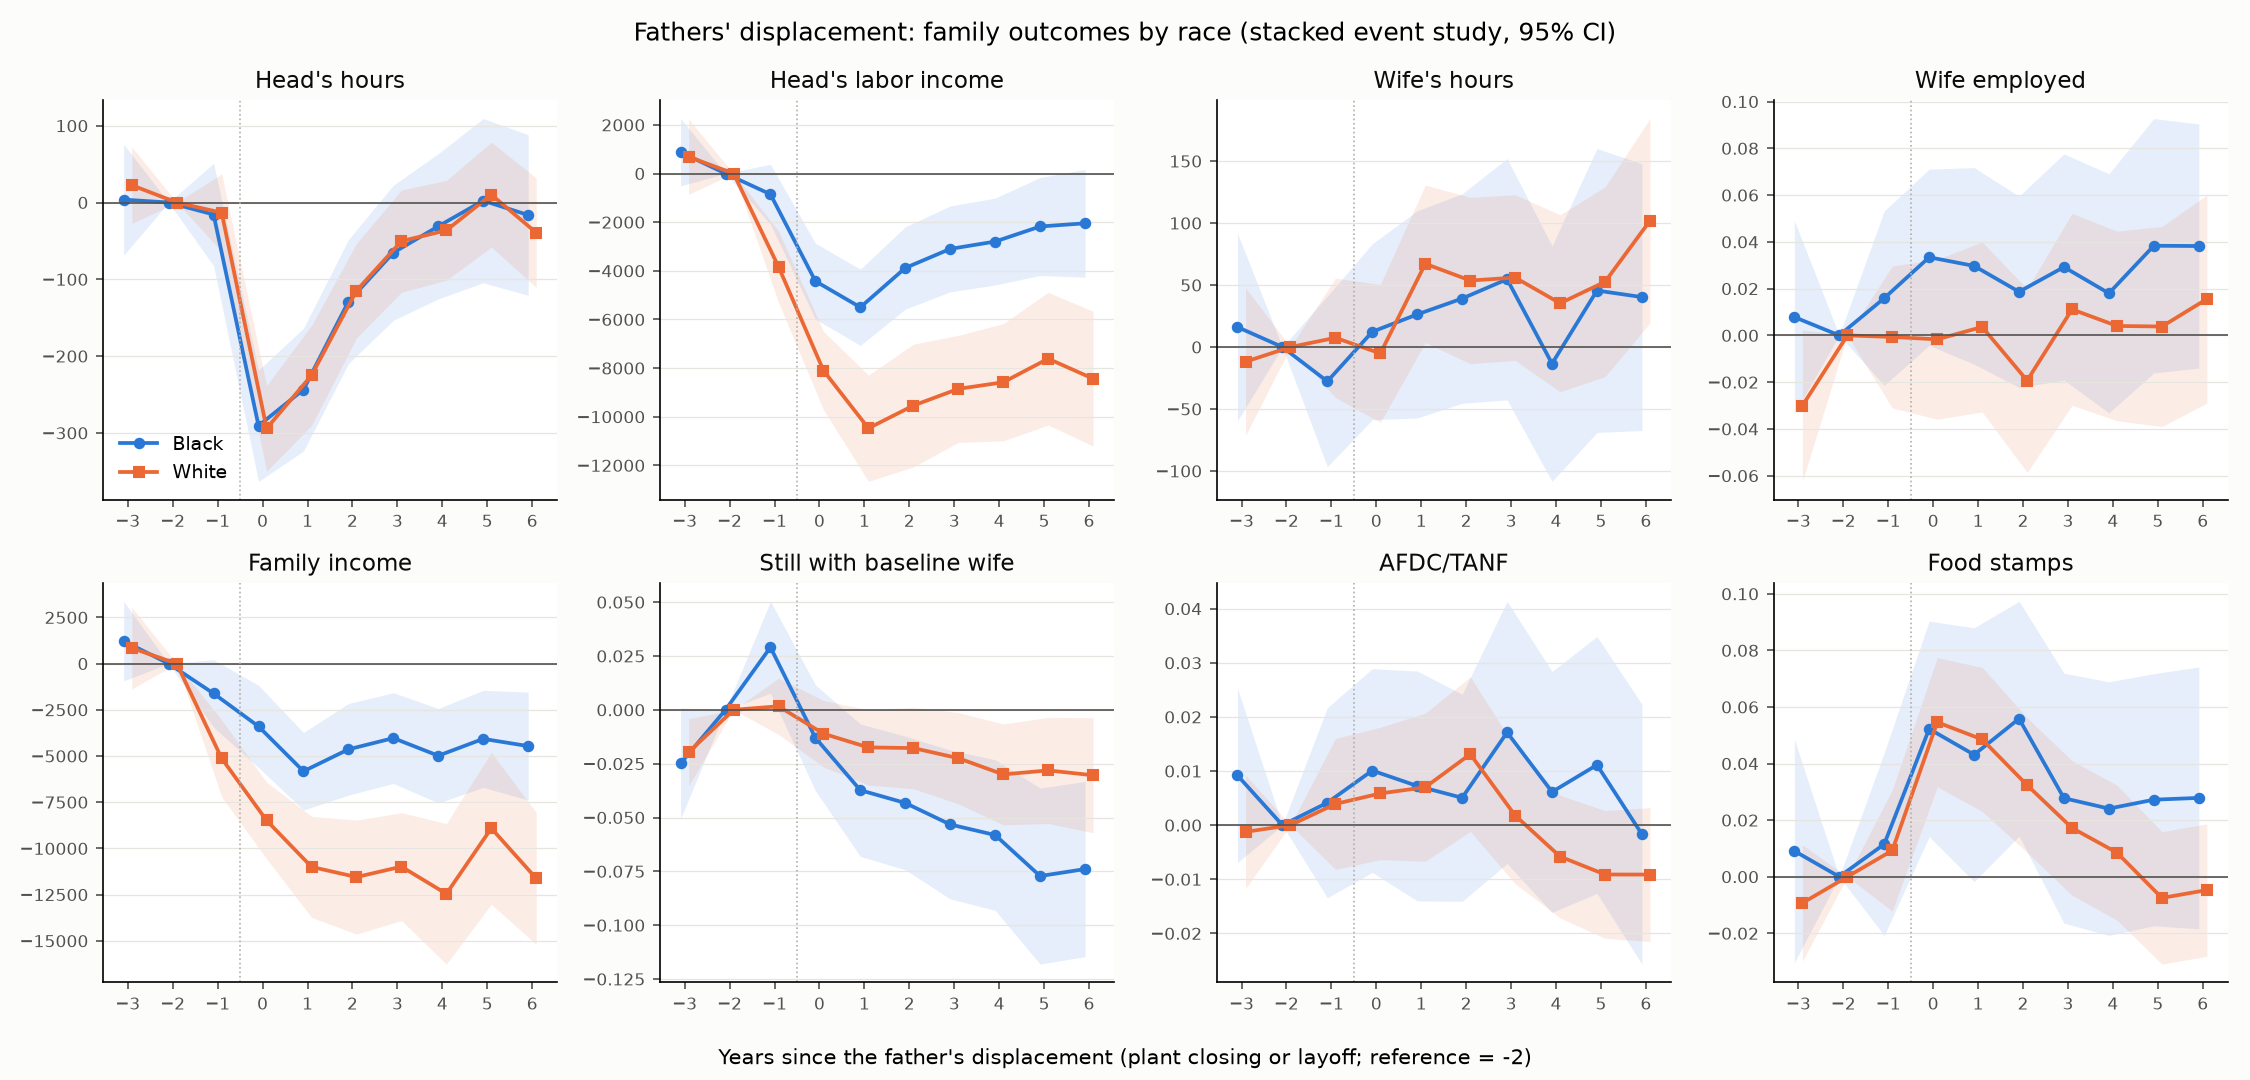
\includegraphics[width=\textwidth]{father_displacement_es.png}
\caption{The father's displacement and the family, by race (PSID)}\label{fig:displacement_es}
\begin{minipage}{0.95\textwidth}\footnotesize Stacked event study, effects by year relative to the displacement
(reference year $-2$), with 95\% confidence intervals; Black and White fathers. Sample and controls as in
Table~\ref{tab:displacement_family}.\end{minipage}
\end{figure}

\subsection{The wife's response: search at once, jobs slowly}

Wives make up a small part of the loss, and mainly when the children are young. On average, a wife works 51 more hours
a year after her husband's job loss, and her employment does not change. When the youngest child is under six, she
works 112 more hours and is 4.1 percentage points more likely to be employed; when the youngest child is of school age,
her hours do not rise and her employment falls by 3.8 points. Black wives respond less than White wives when the
children are young: 68 more hours, not significantly different from zero, against 117 for White wives.

The monthly CPS shows how the response unfolds. Wives who were not working when their husband lost his job begin to
look for work at once: their probability of being unemployed and looking rises by 8.8 points in the month after his job
loss (0.088$^{***}$, on a base of 6.0\%). Jobs come slowly: their probability of being employed rises by 2.2 points after
one month, 4.2 points after three and 4.0 points after twelve (all $p<0.001$). The response is concentrated among
mothers of young children (3.6 points after one month, against 0.4 for wives without children, $p=0.382$) and is larger
for Black wives (4.7 points after one month and 10.0 after twelve, against 1.8 and 3.4 for White wives). Wives who were
already unemployed when their husband lost his job become less likely to find work ($-0.020^{*}$ after one month,
$-0.050^{**}$ after three): their own labor market has been hit too. The SIPP, which follows wives for three years, shows the same
pattern over a longer horizon (Figure~\ref{fig:sipp_wife}): among wives with no job the month before, employment
builds up over about six months, from 1.9 points in the month of the husband's separation to 5.4 points after six
months, and stays about 4.4 points higher after two years. These wives were already more often looking for work before
his separation (4.4 points in the month before), so the SIPP's rise in looking at the separation is small (to 5.3
points); the CPS, which records search in the reference week, shows the jump. Because wives who were working lose their
own jobs in the same months, the net change in all wives' employment is about zero for a year
(Appendix~\ref{app:robust}). The
PSID's annual interview-week status does not show a rise in looking for work a year after the job loss (for all wives $-0.001$, s.e.\ 0.008), because by then the search
spell has ended in a job or in leaving the labor force; the annual snapshot misses what the monthly data show.

\begin{figure}[htbp]\centering
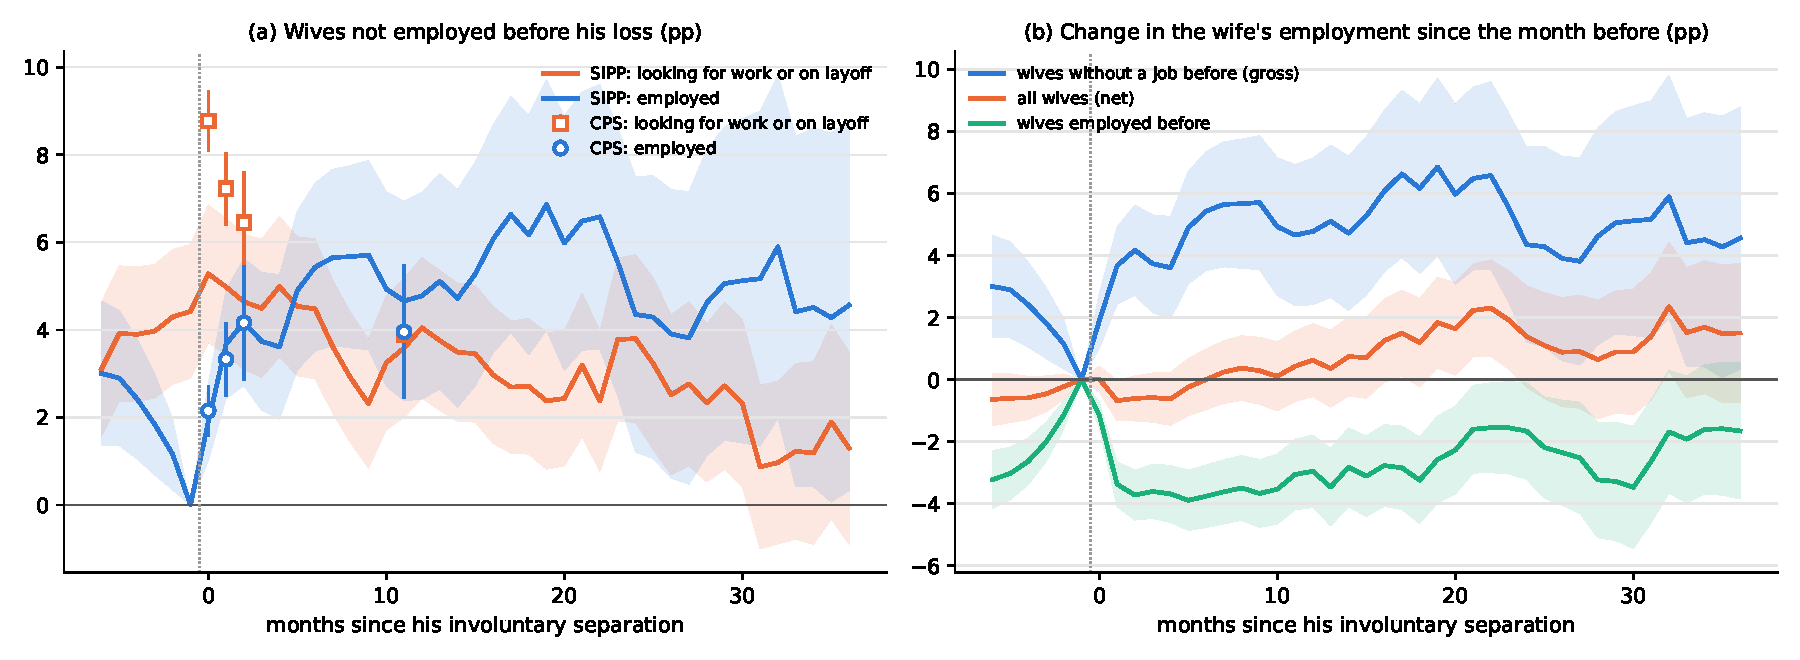
\includegraphics[width=\textwidth]{fig_sipp_wife_response.pdf}
\caption{The wife's response month by month (SIPP and CPS)}\label{fig:sipp_wife}
\begin{minipage}{0.95\textwidth}\footnotesize (a) Wives with no job in the month before the husband's involuntary
separation: difference in the probability of being employed and of looking for work or being on layoff between wives
whose husband separates in month 0 and wives whose husband stays employed, by month (one linear probability model per
month, base panel $\times$ month fixed effects; SIPP 2004, 2008 and 2014 panels). Employed at $s=0$: 1.9$^{***}$
points (s.e.\ 0.5); $s=6$: 5.4$^{***}$ (1.0); $s=24$: 4.4$^{***}$ (1.6, $p=0.007$). Looking: 4.4$^{***}$ (0.8) at $s=-1$, 5.3$^{***}$
(0.8) at $s=0$. Markers: CPS basic monthly 1994--2023, wives not employed in month $t$, husband's job loss at $t+1$,
plotted at $s=k-1$ for $t+k$; state $\times$ month fixed effects; looking at $t+1$: 8.8$^{***}$ (0.4); employed at
$t+3$: 4.2$^{***}$ (0.7) and at $t+12$: 4.0$^{***}$ (0.8). (b) Change in the wife's employment since the month before
his separation: wives without a job before (gross entry), all wives (net) and wives employed before (their own job
loss). 95\% confidence intervals clustered by household. Code: \texttt{40.SIPPJointLoss.py},
\texttt{37.CPSJointLossChecks.py} (\texttt{output/sipp\_joint\_loss.csv}, \texttt{output/cps\_joint\_loss\_checks.csv}).
\end{minipage}
\end{figure}

\subsection{Gross and net added work}

The joint job loss changes how the added-worker response should be read. Average estimates of the added-worker effect
\citep{stephens2002worker, halla2020job} net two groups of wives: those who work more after their husband's job loss and
those who lose their own job with his. The PSID allows the two to be separated from 1984 on, when wives' own job-end
reports begin. Splitting displaced families by whether the wife was herself displaced in the three years around the
husband's job loss, the gross response of wives who kept their jobs is 47 hours a year over years 1 to 3 ($p=0.165$),
and 97 hours when the youngest child is under six ($p=0.032$). Wives who were displaced with their husband work 388
fewer hours ($p=0.003$). Because 10.6\% of the wives of displaced men are displaced themselves, against 5.0\% of the
wives of other men, the joint losses offset 35 hours of the gross response (s.e.\ 14; $p=0.013$), so the net response in
these years is 12 to 16 hours and not significant (Figure~\ref{fig:gross_net}).\footnote{Interaction model in the
stacked event study, event years 1984--2021; the wife's own displacement is observed for 82\% of displaced families
(it is missing when the couple has split or is not interviewed), and conditioning on it is descriptive. The offset
rests on 119 displaced husbands whose wife was also displaced. The average response of 51 hours in
Table~\ref{tab:displacement_family} combines events before 1984 (74 hours, $p=0.029$), when the wife's own job losses
are not measured, with events from 1984 (30 hours, $p=0.364$). Code: \texttt{IGE/38.PSIDJointLossChecks.py}
(\texttt{output/psid\_joint\_loss\_checks.md}).} The joint losses remove more than two thirds of the gross response of
the average wife. The small net response reflects, in large part, not an unwillingness or inability to add work but the
loss of the wife's own job to the same shock. A model of household insurance in which the second earner's job is
independent of the first earner's, or in which only the net response is targeted, overstates what the family can
absorb in the months of the shock.

\begin{figure}[htbp]\centering
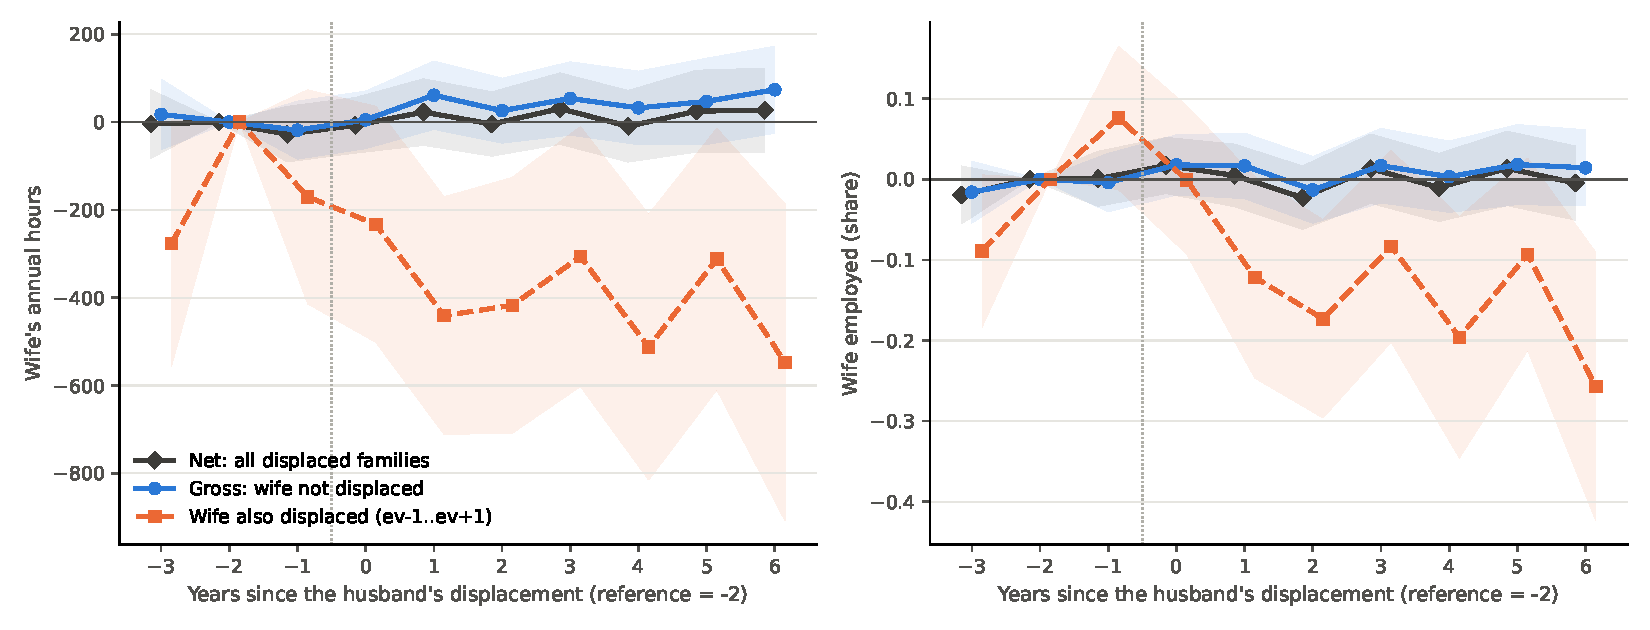
\includegraphics[width=0.85\textwidth]{fig_gross_net_awe.pdf}
\caption{Gross and net added work after the husband's displacement (PSID, 1984--2021)}\label{fig:gross_net}
\begin{minipage}{0.95\textwidth}\footnotesize Wife's annual hours (left) and employment (right) by year relative to the husband's displacement,
for displaced families in which the wife kept her job (gross response), in which she was displaced too, and all
displaced families (net response), relative to control families; 95\% confidence intervals clustered by 1968 family.
Code: \texttt{IGE/38.PSIDJointLossChecks.py}.\end{minipage}
\end{figure}

\subsection{The wife's own labor market and the difference by race}

Beyond the joint job loss, the wife's own labor market at the time of the husband's job loss does not limit her
response: employment growth in her sector, labor demand in her state and the change in her state's unemployment rate do
not weaken it. The racial difference in the response lies among wives who were not working before the husband's job
loss, who enter work after it if they are White and much less if they are Black, although Black wives search more in
the CPS. Black spouses are slightly less alike in industry than White spouses, and joint job losses are equally
frequent, so correlated shocks do not explain this difference. A search friction that is higher for Black women and
preferences, including the value of time with young children, remain as explanations; the model separates them by
their implications for women's search and employment over the life cycle.

\subsection{The marriage}

The job loss also strains the marriage. The share of displaced fathers still living with the wife they had before the
job loss falls by 4.5 percentage points over years 1 to 3 for Black fathers and by 1.9 points for White fathers, and the
gap keeps widening: by year 6 it is 7.4 points for Black fathers (s.e.\ 2.1) and 3.0 points for White fathers (s.e.\
1.4). The divorce response to job loss is known \citep{charles2004job}. The point estimates are about twice as large
for Black as for White fathers, but the racial difference is not statistically significant, and with plant closures
only the response is similar to that after layoffs (Black $-0.044$, $p=0.108$, against $-0.044^{**}$ after layoffs;
White $-0.015$, $p=0.304$, against $-0.021^{*}$), so the distinction between layoffs and closures that
\citet{charles2004job} find does not appear here.\footnote{Closures-only and layoffs-only versions of every outcome of
Table~\ref{tab:displacement_family}, by race and by child age: \texttt{output/psid\_joint\_loss\_checks.md},
Section 2. With closures only, wives' hours rise by 83 ($p=0.040$), and by 210 when the youngest child is under six
($p<0.001$).}

The wife's own job loss strains the marriage as much, as \citet{charles2004job} found, and their result for wives
that layoffs matter and plant closings do not reappears here. With the roles reversed, so that the event is the wife's first
displacement (wives of male heads with children who worked before; events 1984--2021), the probability that she is
still with the husband she had before falls by 4.6 percentage points over years 1 to 3 ($-0.046^{***}$, s.e.\ 0.012)
and by 9.0 points over years 4 to 6 ($-0.090^{***}$, s.e.\ 0.016), among 1,205 displaced wives; by 4.8 points for Black
wives ($p=0.037$) and 4.0 points for White wives ($p=0.005$), a difference of 0.008 ($p=0.77$). Her hours fall by 127 a
year over years 1 to 3 and are back by years 4 to 6, while the gap in the marriage keeps widening. Estimated in one
regression with the husband's displacement over the same event years, the two responses do not differ ($-0.046$
against $-0.036$ over years 1 to 3, difference $p=0.54$; $-0.090$ against $-0.051$ over years 4 to 6, $p=0.061$). In
three of five of these break-ups it is the husband who leaves the family. A joint loss, both spouses displaced within a
year, gives the largest response: over the six years after the husband's displacement, the share still together is 9.5
points lower when his wife lost her job too ($-0.095^{***}$, $p=0.009$) and 4.1 points lower when she kept hers
($-0.041^{***}$); with 174 joint events the difference is not statistically significant ($p=0.15$). The response
survives baseline characteristics interacted with event time ($-0.033^{***}$ over years 1 to 3), dropping the couples
who lost both jobs, and requiring that both displaced and control wives be interviewed when the job loss would be
reported ($-0.050^{***}$). Two caveats remain. As for the husband's displacement, the outcome equals one before the
job loss by construction, so there is no pre-period placebo. And plant closures alone give a smaller response that is
not significant ($-0.027$, $p=0.19$, 376 closures; layoffs and firings $-0.056^{***}$), and displaced wives were
younger and in shorter marriages than the controls, so part of the response after layoffs and firings may reflect who
is laid off.\footnote{Code: \texttt{IGE/64.SeparationUIAndHerLoss.py} (main estimates) and
\texttt{IGE/65.HerLossRobustness.py} (checks); output \texttt{output/her\_loss\_robustness.md}. Same stacked design
as Table~\ref{tab:displacement_family}, standard errors clustered by 1968 family; events include her own reports as a
female head after a separation, so they are not conditioned on staying married. Her versus his, both designs stacked
in one regression with one clustered covariance; among couples in which both worked before, $-0.044^{***}$ against
$-0.043^{***}$ (difference $p=0.95$). Closures minus layoffs over years 1--6: wife 0.049 ($p=0.082$), husband 0.025
($p=0.33$); with baseline controls, closures $-0.021$ ($p=0.31$). Baseline balance (displaced minus control within
stacks): she is 2.1 years younger, her earnings are \$7,149 lower and his \$10,062 lower, 13 points more of the
couples have been observed together for two years or less (all $p<0.001$); her share of the couple's earnings is the
same ($-0.009$, $p=0.24$); her hours and earnings show no trend before the event (earnings at $e=-3$ and $e=-1$: 455,
$p=0.50$; $-425$, $p=0.39$). Dropping the 244 wives whose husband was displaced within a year of her: $-0.049^{***}$
(years 1--3), $-0.081^{***}$ (4--6); joint against her loss alone over years 1--6, $-0.083^{**}$ against $-0.070^{***}$
(difference $p=0.74$); in the husband's design, joint $-0.095^{***}$ against his loss alone $-0.041^{***}$
(difference $p=0.15$, 174 joint events). By her share of the couple's earnings (above or below the median of 0.36, or
0.40), the responses do not differ ($p \geq 0.33$), although her hours fall by 270 when her share was above the median
and not at all below it. Who leaves (no reason for a separation is recorded): the husband moves out in 60\% of first
separations after her displacement and 65\% among controls, she moves out in 15\% and 16\%, and his death plays no part
($-0.002$, $p=0.44$). Requiring both groups to be interviewed at the first interview after the event year (a displaced
wife must be to report the job loss) makes later attrition equal (0.011, $p=0.36$); filling the outcome from his side
when she is not interviewed then gives $-0.051^{***}$.}

The insurance that survives the marriage is hit as well. A separated mother with children receives \$132 (Black) or
\$327 (White) a month in child support on average; when her husband had been displaced in the two years before the
separation, she receives \$116 a month less ($-116^{***}$, $p<0.001$; Black $-88^{***}$, White $-155^{***}$), and her
food-stamp receipt is 11.4 points higher ($+0.114^{***}$). The father's job loss that precedes the break-up also cuts
the transfer that is meant to replace his earnings after it.\footnote{PSID mothers whose marriage ended in 1984--2020
(marriage-history dates), seen married with a child under 18 in the three years before the separation, aged 25--59;
570 Black and 924 White mothers; outcomes in the ten years after the separation while single. Standard errors
clustered by 1968 family. The comparison with mothers whose husband was not displaced is descriptive. Remarriage is
not lower after his displacement (0.000, $p=0.94$). Code: \texttt{IGE/76.SeparatedMothers.py}; output
\texttt{output/separated\_mothers.md}.}

\subsection{Consumption}

Consumption is measured in the PSID from 1999, so this evidence covers 1999--2021 only. I construct the measure of
\citet{blundell2016consumption}---nondurable goods and services, with a rent equivalent of 6\% of the house value for
owners---for every wave from 1999 to 2021; for 1999--2009 it reproduces their series exactly.\footnote{Items are found in
each wave by their PSID labels; question changes (heating, health insurance premiums, health spending, car repairs,
time units) are harmonised, a combined gas and electricity bill asked from 2007 is added to utilities, and the
categories added in 2005 (clothing, trips, recreation, home repairs, furnishings) are excluded from the consistent
series. Stacked event study as in Table~\ref{tab:displacement_family}, events 2000--2020, event time in interview waves;
standard errors clustered by 1968 family. Code: \texttt{IGE/47.PSIDConsumptionEvent.py}
(\texttt{output/psid\_consumption\_event.md}).} Among 548 displaced husbands, 63 of whose wives were displaced in the
three years around his job loss, consumption barely falls after the husband is displaced alone: by 1.3\% over the first
three interviews after the job loss ($p=0.49$) and 3.2\% at the first ($p=0.13$). After a joint displacement it falls by
7.1\% ($p=0.31$); the difference from a single displacement is $-0.059$ (s.e.\ 0.073, $p=0.42$), $-0.127$ excluding housing
($p=0.14$) and $-0.170$ for food ($p=0.13$) (Figure~\ref{fig:consumption}). Because the wife's job loss can precede her
husband's, the last interview before his job loss can already follow hers; measured against the interview before
that, consumption falls by 21.4\% after a joint displacement ($p=0.025$) and by 18.5 points more than after a single one
($p=0.058$), on 26 joint events. The household's consumption is well insured against the husband's job loss alone; the
point estimates indicate a larger fall when both earners are lost, but with 63 joint events in two-year interview data
the difference is not precisely estimated, as in the panel of \citet{blundell2016consumption}. The model uses the
consumption response to a single displacement as a target for 1999--2021 and the joint-minus-single difference as a
target with its standard error.

\begin{figure}[htbp]\centering
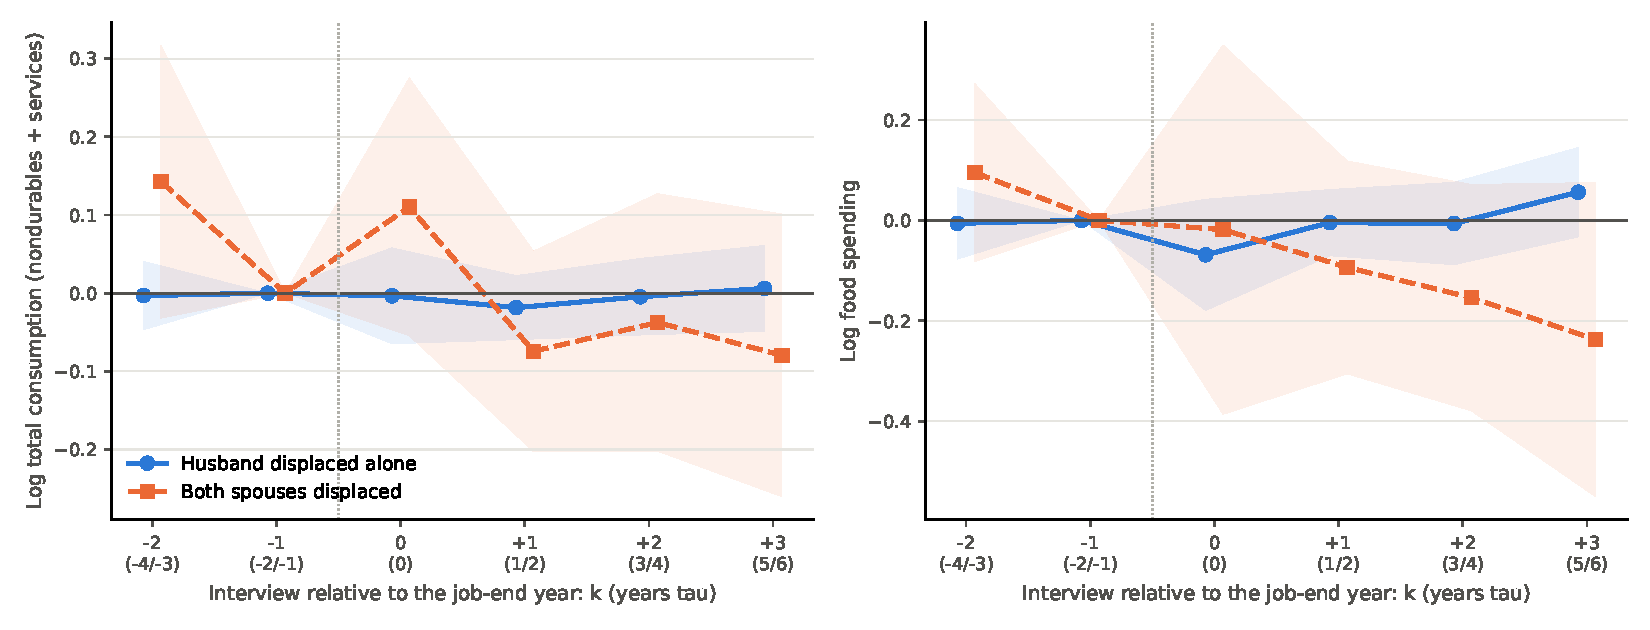
\includegraphics[width=\textwidth]{fig_consumption_single_joint.pdf}
\caption{Consumption around single and joint displacements (PSID, 1999--2021)}\label{fig:consumption}
\begin{minipage}{0.95\textwidth}\footnotesize Log total consumption (nondurables and services, left) and log food
spending (right) by interview relative to the husband's job-end year, for husbands displaced alone and couples in which
both spouses were displaced, relative to couples without a displacement (reference: the last interview before the job
loss); 95\% confidence intervals clustered by 1968 family. Code: \texttt{IGE/47.PSIDConsumptionEvent.py}.\end{minipage}
\end{figure}

\subsection{The safety net}

Food stamp receipt rises by 4.2 points for Black and 3.3 points for White families after the father's displacement,
while AFDC/TANF receipt barely moves. The joint job loss determines which programs can respond, and the monthly SIPP
shows how. When the husband loses his job alone, unemployment insurance reaches him at once: his receipt rises by 23
points in the first three months and stays 13 points higher half a year later, and the couple almost never goes
without both earnings and benefits (1.0\% of couple-months in the first half year). When the wife loses her job too,
his benefits rise by about as much, hers rise by 11 to 18 points, and yet 9.3\% of the couple-months in the first half
year have no earner and no unemployment insurance, 5.7 points more than after his loss alone.\footnote{SIPP panels
2004, 2008 and 2014 (reference months 2003--2016): dual-earner couples with the wife aged 25--59, both employed in
the month before the husband's involuntary separation (layoff, closure, discharge or end of a temporary job) at
$s = 0$; a joint loss is an involuntary separation of the wife in $s = -3, \dots, +3$ (206 events, against 2{,}644
losses of his alone). Clean controls: 29{,}899 couples with a pseudo-event month in which both work and neither
spouse separates involuntarily nearby. Regressions on event month $\times$ group with couple and panel $\times$
rotation $\times$ calendar-month fixed effects, reference $s = -3, \dots, -1$, standard errors clustered by household
(32{,}109 clusters, $N = 516{,}624$). His UI receipt: $+22.6^{***}$ points (s.e.\ 0.7) in $s = 0$--$2$ and
$+13.3^{***}$ (0.7) in $s = 6$--$11$ after his loss alone; $+18.2^{***}$ (2.5) and $+9.7^{***}$ (2.5) after a joint
loss. Her UI receipt after a joint loss: $+10.9^{***}$ (2.1) in $s = 0$--$2$ and $+18.0^{***}$ (2.7) in $s = 3$--$5$.
No earner and no UI: $+6.2^{***}$ (1.4) and $+6.4^{***}$ (1.7) after a joint loss, $+0.5^{***}$ (0.1) and
$+0.7^{***}$ (0.2) after his loss alone; joint minus alone $+5.7^{***}$ (1.7; $p<0.001$) in $s = 3$--$5$ and
$+2.6^{*}$ (1.3; $p=0.055$) in $s = 6$--$11$. Receipt is from the core-wave program items (2004/08: state UI ER05 /
T05AMT, household food stamps THFDSTP, own receipt and coverage ER27, RCUTYP27; 2014: EUC1--3MNYN, RFSYN, RFSCOV).
The employment pre-trend ($-5.9^{***}$ in $s = -6$ to $-4$) follows from requiring both spouses to work at $s = -1$
(\texttt{IGE/78.SafetyNetJointLoss.py}).} In the couple-months of a joint loss in which neither spouse works, which
are a quarter of the first half year, 39\% receive unemployment insurance for neither spouse and 23\% receive neither
unemployment insurance nor food stamps.\footnote{Couple-months $s = 1$--$6$ after a joint loss with both spouses
not employed: 24.0\% of the joint-loss couple-months (1.5\% after his loss alone); among them UI for neither spouse
38.7\%, food stamps 33.8\%, neither program 23.5\% (316 couple-months). After his loss alone, among couple-months with
him not employed: UI for neither 51.2\%, food stamps 9.7\% (6{,}458 couple-months). Weighted by the wife's weight in
$s = -1$ (\texttt{IGE/78.SafetyNetJointLoss.py}).}

Food stamps respond less than the joint loss would suggest, because the couples who lose both jobs are already the
couples on the program. In the three months before his loss, 19\% of joint-loss couples receive food stamps, against
5.9\% of couples in which he loses his job alone and 3.2\% of the controls; receipt then rises by 1.0 to 1.5 points after
his loss alone and by 1 to 3 points, imprecisely, after a joint loss. AFDC/TANF does not move in either
group.\footnote{Food stamp receipt relative to $s = -3, \dots, -1$: after his loss alone $+1.05^{***}$ (0.26) in
$s = 0$--$2$, $+1.51^{***}$ (0.36) in $s = 3$--$5$, $+1.40^{***}$ (0.43) in $s = 6$--$11$; the amount rises by
\$3.9--5.2 a month (2000 dollars, zeros included). After a joint loss $+1.14$ (1.25; $p=0.361$), $+3.28$ (2.23;
$p=0.141$), $+3.26$ (2.61; $p=0.212$); joint minus alone $+1.77$ (2.26; $p=0.434$) in $s = 3$--$5$. TANF receipt:
$+0.12$ (0.08; $p=0.138$) and $+0.16$ (0.58; $p=0.779$) in $s = 0$--$2$. In the PSID couple-years (25's intervals,
1984--2021), food stamps are received in the year before by 15.6\% of joint-loss couples, 10.5\% after his
displacement alone and 3.4\% when neither spouse is displaced; the change over the interval relative to couples with
no displacement is $+1.88^{***}$ points (0.57) after his displacement alone and $+5.24^{**}$ (2.18; $p=0.016$) after a
joint one, and AFDC/TANF does not change ($+0.17$, $p=0.571$; $+0.11$, $p=0.932$); calendar-year fixed effects, 1968
family clusters, $N = 60{,}061$ (\texttt{IGE/78.SafetyNetJointLoss.py}).}

An earnings subsidy such as the Earned Income Tax Credit pays nothing in a month in which neither spouse works, and
these are the months the joint loss adds. Over the calendar year the schedule acts the other way. Before the loss,
most dual-earner couples earn too much for the credit, and the fall in annual earnings moves some of them into its
range. Applying the married-joint schedule of the era to the PSID couples' earnings, 24\% of joint-loss couples are in
the credit range in the year before and 34\% at the end of the interval. 8.3\% end in the phase-in region or with no
earnings, where the credit falls with every lost dollar, against 3.8\% after his displacement alone. The schedule
credit rises by \$196 a year relative to couples without a displacement, against \$66 after his displacement alone.
The subsidy pays least to the couples whose joint loss lasts long enough to empty a year of earnings. For the others
it is a partial, delayed insurance against the loss of annual income.\footnote{Schedule of
\texttt{IGE/61.PolicySchedules.py} (era means, 2000 dollars, married filing jointly, children capped at three),
applied to the sum of both spouses' annual labor incomes; no AGI or investment-income test, no take-up, so this
places the couple on the schedule and does not measure receipt. Year before = the interview opening the interval,
end = the interview closing it (one year to 1996, two after). Shares at the end of the interval for joint-loss
couples: no earnings 0.9\%, phase-in 7.4\%, plateau 4.6\%, phase-out 21.2\%, above the range 66.0\% (326 couple-years).
LPMs on displacement groups relative to couples without a displacement, calendar-year fixed effects, 1968 family
clusters, $N = 60{,}061$: change in the schedule credit $+\$195.7^{***}$ (48.8) joint, $+\$65.8^{***}$ (11.6) his
alone, difference $+\$129.9^{***}$ (49.1; $p=0.008$); entering the phase-in region or no earnings $+4.86^{***}$
points (1.36) joint, $+1.69^{***}$ (0.36) his alone, difference $+3.17^{**}$ (1.40; $p=0.023$). Black couples: credit
$+\$287^{**}$ (115) joint, entering phase-in or no earnings $+8.33^{***}$ (2.92); White couples: $+\$153^{***}$ (45)
and $+3.10^{**}$ (1.42). Annual intervals only (1984--1996): credit $+\$141^{***}$ (39) joint, $+\$55^{***}$ (10) his
alone (\texttt{IGE/78.SafetyNetJointLoss.py}).} Unemployment insurance covers each spouse only if he or she
qualifies, so a joint loss can leave one of the two uncovered: in nearly four in ten joint-loss months without an earner,
neither spouse draws it.

\section{The Children}\label{sec:children}

The joint job loss and the household's response determine what reaches the children: a family income that stays lower
for years, a higher risk that the parents separate, and, in the month of the shock, a household with no earner. This
section reports what the PSID can say about the children's adult outcomes. The answer is a set of associations that
bound, rather than identify, the effect of a father's job loss; the model uses them as bounds, together with
administrative estimates.

\paragraph{Associations.} I compare children whose father figure was displaced at a given age with children whose
father figure was not, controlling for parental income before the displacement, the child's sex and birth year
(Table~\ref{tab:displacement_children}). A displacement before age six is associated with a household income rank 3.9
percentiles lower and 0.28 fewer years of schooling; a displacement at 12--17 with adult earnings about 14\% lower, a
rank 2.5 percentiles lower and 0.29 fewer years of schooling. For White children most of these associations are
statistically significant; for Black children they are significant mainly for displacements at 12--17, and the
estimates are imprecise. Adding family income after the displacement reduces the associations by about a third,
while adding the change in the mother's hours changes nothing; both are outcomes of the job loss, so this split is
descriptive.\footnote{\texttt{IGE/output/father\_displacement.md}; code \texttt{IGE/20.PaperDisplacement.py}.}

\begin{table}[htbp]\centering\small
\caption{The father's displacement and children's adult outcomes}\label{tab:displacement_children}
\resizebox{\textwidth}{!}{%
\begin{tabular}{lcccc}
\toprule
 & \begin{tabular}[b]{@{}c@{}}(1) Log\\lifetime earnings\end{tabular} & \begin{tabular}[b]{@{}c@{}}(2) Log lifetime\\family income\end{tabular} & \begin{tabular}[b]{@{}c@{}}(3) Family\\income rank\end{tabular} & \begin{tabular}[b]{@{}c@{}}(4) Years\\of schooling\end{tabular} \\
\midrule
\multicolumn{5}{l}{\textit{A. All children}} \\
Father displaced at 0--5 & $-0.058$ & $-0.086^{***}$ & $-3.91^{***}$ & $-0.279^{***}$ \\
 & (0.040) & (0.030) & (1.15) & (0.072) \\
Father displaced at 6--11 & $-0.075$ & $-0.057^{*}$ & $-3.63^{***}$ & $-0.312^{***}$ \\
 & (0.046) & (0.031) & (1.24) & (0.079) \\
Father displaced at 12--17 & $-0.154^{***}$ & $-0.065^{**}$ & $-2.51^{**}$ & $-0.294^{***}$ \\
 & (0.053) & (0.028) & (1.04) & (0.076) \\
\multicolumn{5}{l}{\textit{B. Black children}} \\
Father displaced at 0--5 & $-0.001$ & $-0.057$ & $-2.54$ & $-0.117$ \\
 & (0.071) & (0.056) & (1.87) & (0.104) \\
Father displaced at 6--11 & $-0.048$ & $-0.003$ & $-2.07$ & $-0.041$ \\
 & (0.087) & (0.059) & (2.17) & (0.124) \\
Father displaced at 12--17 & $-0.189^{*}$ & $-0.090$ & $-3.35^{*}$ & $-0.317^{***}$ \\
 & (0.101) & (0.061) & (1.98) & (0.122) \\
\multicolumn{5}{l}{\textit{C. White children}} \\
Father displaced at 0--5 & $-0.084^{*}$ & $-0.101^{***}$ & $-4.48^{***}$ & $-0.364^{***}$ \\
 & (0.047) & (0.035) & (1.44) & (0.095) \\
Father displaced at 6--11 & $-0.102^{*}$ & $-0.089^{**}$ & $-4.68^{***}$ & $-0.511^{***}$ \\
 & (0.054) & (0.037) & (1.52) & (0.102) \\
Father displaced at 12--17 & $-0.137^{**}$ & $-0.057^{*}$ & $-2.47^{**}$ & $-0.324^{***}$ \\
 & (0.062) & (0.030) & (1.22) & (0.098) \\
\bottomrule
\end{tabular}}
\begin{minipage}{0.95\textwidth}\footnotesize Each coefficient is from a separate regression of the outcome in the column on an indicator that the child's father figure (the male head of the child's family) had his first displacement when the child was in the age band of the row, against children whose father figure was not displaced; children first exposed in another band are dropped. Controls: log parental income before the displacement, child sex, Black (pooled panel) and birth-year fixed effects. Adult outcomes are means over ages 25--55 (ranks within birth cohort). Associations, not causal effects. Standard errors clustered by 1968 family. *** $p<0.01$, ** $p<0.05$, * $p<0.1$.\end{minipage}
\end{table}


\paragraph{How much is the job loss.} Displaced families differ before the job loss: their family income is 24 log
points lower, the parents have 0.6 fewer years of schooling, and the father's earnings were already growing more slowly
(all $p<0.01$). Controlling for the father's earnings path, occupation and industry barely changes the associations, but
four checks narrow what can be attributed to the job loss. With plant closures alone the associations vanish for Black
children (adult earnings $+0.085$, s.e.\ 0.078) and survive for White children's schooling ($-0.40$ years, s.e.\ 0.11)
and earnings rank ($-3.3$ percentiles, s.e.\ 1.6). A displacement after the child has left childhood (at 18--25) is not
associated with schooling ($-0.08$, s.e.\ 0.09), while one at 12--17 is ($-0.27$, s.e.\ 0.08; difference $p=0.060$).
The behavior problems of younger children are elevated before the displacement, so that association reflects the
families rather than the job loss. Quits also predict less schooling (Table~\ref{tab:displacement_definitions}), which
signals selection. The main definition reproduces the association of about $-9\%$ in adult earnings found by
\citet{page2009parental} in the PSID.\footnote{Comparisons of siblings are not used: siblings share and compete for the
family's resources and influence each other, and a job loss also affects later-born siblings through the family's
lasting income loss, so they are not a clean control. Code: \texttt{IGE/22.DisplacementID.py}.}

\begin{table}[htbp]\centering\small
\caption{Definitions of the father's job loss}\label{tab:displacement_definitions}
\resizebox{\textwidth}{!}{%
\begin{tabular}{lccc}
\toprule
 & \begin{tabular}[b]{@{}c@{}}(1) Log\\lifetime earnings\end{tabular} & \begin{tabular}[b]{@{}c@{}}(2) Log lifetime\\family income\end{tabular} & \begin{tabular}[b]{@{}c@{}}(3) Years\\of schooling\end{tabular} \\
\midrule
Closure or layoff (main) & $-0.092^{***}$ & $-0.079^{***}$ & $-0.431^{***}$ \\
 & (0.033) & (0.023) & (0.058) \\
Closures only & $-0.080^{*}$ & $-0.060^{**}$ & $-0.273^{***}$ \\
 & (0.042) & (0.030) & (0.077) \\
Quits (placebo) & $-0.065^{*}$ & $-0.020$ & $-0.296^{***}$ \\
 & (0.039) & (0.030) & (0.071) \\
Year without hours (earlier measure) & $-0.154^{***}$ & $-0.150^{***}$ & $-0.408^{***}$ \\
 & (0.047) & (0.034) & (0.075) \\
\bottomrule
\end{tabular}}
\begin{minipage}{0.95\textwidth}\footnotesize Exposure at child ages 0--17, all children; controls as in Table \ref{tab:displacement_children}. *** $p<0.01$, ** $p<0.05$, * $p<0.1$.\end{minipage}
\end{table}


\paragraph{What the model takes from this.} The PSID associations are an upper bound on the total effect of a father's
job loss on his children. They are robust only for White children's schooling and for job losses during childhood.
Administrative data find smaller effects: about $-9\%$ in adult earnings in Canada
\citep{oreopoulos2008intergenerational}, and much less in US tax data. There, a father's layoff during adolescence
cuts family income sharply, lowers college enrollment by less than half a percentage point, and leaves early-career
earnings almost unchanged \citep{hilger2016parental}. The model's child block maps family income at ages 0--5 and
6--17, and the share of childhood spent with both parents, into adult log earnings. The income slopes are set so that
a father's displacement at the mean displacement age lowers his child's adult earnings by 9\% (the high slope) or by
0.35\% (the low slope, from the US estimates of the working-paper version of \citet{hilger2016parental}, college quality measured by alumni earnings). Counterfactuals are reported under both. The presence slope comes from
the PSID. Holding family income at both childhood ages fixed, a childhood spent entirely with both parents is not
associated with higher adult earnings ($+0.011$, s.e.\ 0.045, $p=0.80$). It is associated with 0.30 more years of
schooling ($p<0.001$). Holding fixed only the family's income in the three years before and after the father's
displacement, the association with adult earnings is $0.19^{***}$. The model uses 0.19 as the high presence slope
and zero as the low one.\footnote{PSID children born 1968--1995 (SRC and SEO, unweighted) with at least three
childhood interviews. ``Both parents present'' means the head and the wife of the child's family unit are the child's
mother and father at birth. The share of childhood with both parents averages 0.38 for Black and 0.70 for White
children. Adult earnings are the mean over the years as head or wife at 25--55 (at least three years; zeros kept).
All regressions control for sex, birth year, parental education and, in pooled rows, race. Standard errors are
clustered by 1968 family; siblings are not compared. Without income controls, a childhood with both parents is
associated with adult earnings 29.5 log points higher ($0.295^{***}$, s.e.\ 0.041; $N=5{,}091$), with an earnings
rank 9.5 percentiles higher ($9.46^{***}$) and with 0.72 more years of schooling ($0.724^{***}$). Net of log family
income at 0--5 and 6--17, the earnings coefficient is $0.011$ (s.e.\ 0.045, $p=0.80$; $N=4{,}701$): Black $-0.031$
($p=0.65$), White $0.069$ ($p=0.24$). The schooling coefficient is $0.299^{***}$ (s.e.\ 0.081; $N=6{,}213$): Black
$0.213^{*}$ ($p=0.054$), White $0.476^{***}$. The income slopes in that regression are $0.148^{***}$ (ages 0--5) and
$0.320^{***}$ (6--17) for log earnings; they are associations, which is why the model takes its income slopes from
administrative estimates instead. Splitting the shares by age, the share with both parents at 6--17 is positive for earnings
($0.102^{**}$, $p=0.038$) and schooling ($0.342^{***}$). The share at 0--5 is negative for earnings ($-0.126^{**}$,
$p=0.032$) and not significant for schooling ($-0.080$, $p=0.41$). The two age shares are strongly collinear, and
their sum is close to the undivided coefficient. In the father's
displacement sample of Section~\ref{sec:children} (pooled, $N=3{,}520$), the regression of adult log earnings on the
displacement, the share with both parents, and log family income before and after the (pseudo) event gives
displacement $-0.040$ ($p=0.25$), presence $0.187^{***}$ (s.e.\ 0.054), income before $0.179^{***}$ and income after
$0.209^{***}$. Black and White estimates are $0.178^{**}$ ($p=0.037$) and $0.175^{**}$ ($p=0.013$). Without the
income after the event, the presence coefficient is $0.242^{***}$ and the displacement coefficient $-0.084^{**}$
($p=0.016$). Code: \texttt{IGE/79.ParentsPresentOutcomes.py}.} The parents' side of the model is estimated without
the child block, so its results for consumption and for the ranking of policies stand on their own.

\section{A Two-Earner Model of Undiversified Family Insurance}\label{sec:model}

\providecommand{\E}{\mathbb{E}}

The evidence identifies the pieces: a joint job loss that is a same-month coincidence carried by shared workplaces, a
smaller permanent part shared by couples who hold risky jobs, a wife who searches at once and finds work slowly, a
marriage that is strained, consumption insured against one job loss and perhaps not against two, and a safety net
whose programs pay in different states. A model is needed to put them together, to measure what the correlation costs
the household in the months of the shock, and to evaluate policies the data cannot vary. This section sets out the
model to be estimated; the estimates, the fit and the counterfactuals follow in the next version of the paper.

The period is a month: the joint loss is a coincidence within the month (Figure~\ref{fig:cps_hazard}), the wife's
response builds up over about six months (Section~\ref{sec:household}), unemployment insurance lasts 26 weeks, and
most of the earnings risk of US workers is month-to-month and masked in annual data \citep{ganong2026earnings}. In an
annual period the common and the permanent components of the risk collapse into one same-year correlation. The
closest model is the monthly life-cycle model of joint search of \citet{bacher2025joint}, whose labor-market
block---employment and non-employment with and without unemployment insurance that expires at a constant hazard, a
human capital level for each spouse that accumulates at work and depreciates out of it, savings, and extreme-value
taste shocks solved with the endogenous grid method---is followed here. The model departs from theirs in three ways.
The spouses' displacement risk has a common and a permanent couple component, where their separation shocks are
independent across spouses, which bounds the ratio of the wife's job-loss probability in her husband's loss month to
other months at about 1.25 against about 10 in the CPS.\footnote{With independent hazards that depend only on the
human capital level, the ratio is $1 + \mathrm{cov}(\delta_w, \delta_h)/(\E\delta_w\,\E\delta_h)$; with their hazards
between 1.0\% and 5.0\% a month and a mean near 2\%, perfectly correlated levels give at most about 1.25.} The search
friction is exogenous and race-specific, where their job-finding rates are set by firms. And the government is a set
of schedules---a progressive tax, the Earned Income Tax Credit, food stamps and a consumption floor besides
unemployment insurance---the couple has children whose ages set the cost of the wife's work, the marriage can end, and
couples differ by race. All endogenous parameters are estimated jointly by the simulated method of moments, where
theirs are calibrated.

\subsection{Environment and timing}

\paragraph{Households and time.} The economy is populated by married couples. A couple enters the model in January of
the first calendar year in which the corresponding PSID couple is observed and is followed until the wife is 60: with
the wife aged 25 at the earliest, $t = 0, \dots, 419$ indexes months, and $t$ is a multiple of 12 in every January, so
model years are calendar years. Money is in 2000 dollars a month. The couple is a unitary household that maximises one
utility function in which the spouses share consumption and each spouse's work enters as a disutility; the joint-loss
moments carry no information on a Pareto weight. After a separation the wife is the only decision maker of her
household and the husband leaves the model.

\paragraph{Heterogeneity.} Couples differ in four permanent characteristics, all known to the couple. Race
$r \in \{B, W\}$ enters only through the environment---the displacement hazards, the search friction, the separation
hazard, the initial conditions and the inputs---never through preferences, because the joint loss is the same in both
races while the environment differs (Section~\ref{sec:jointloss}); common preferences make the racial differences in
the wife's response a test of the environment. The workplace match $s \in \{0, 1, 2\}$ sets the common component of
displacement risk: $s = 2$ if the spouses share a detailed industry, a detailed occupation and a class of worker (the
closest the public data come to a shared employer), $s = 1$ if they share a detailed industry but not that cell, and
$s = 0$ otherwise.\footnote{CPS: the wife's same-month excess is 0.337 (s.e.\ 0.015) in the shared-employer cell
(6.3\% of couples, 35\% of the raw excess), 0.211 (s.e.\ 0.009) in the same detailed industry (17.7\%, 53\%) and 0.026
(s.e.\ 0.001) outside the shared-employer cell; if 10--12\% of dual-earner couples work at the same establishment
\citep{hyatt2019coworking}, a shared employer carries a third to a half of the excess. The PSID couple's $s$ at entry
is coded with the CPS definition (\texttt{IGE/60.PaperATargets.py}; CPS: \texttt{IGE/37.CPSJointLossChecks.py}).} A
couple risk type $\tau \in \{L, H\}$ scales both spouses' own hazards and stands for the assortative part of the risk:
wives of men who will be displaced four to six years later are already more often displaced
(Table~\ref{tab:joint_job_loss}), and the CPS elevation in the months around his loss is flat, as a permanent type
predicts. Marital status changes once at most. Education does not index the solution: it enters through each spouse's
initial human capital level and initial wealth.

\paragraph{Choices and timing.} Each month the household chooses consumption and saving subject to a borrowing limit,
the wife's hours $\ell_w \in \{0, P, F\}$ when she has a job (zero means she leaves it), the husband's hours
$\ell_h \in \{P, F\}$ when he has a job, and whether to take up food stamps when eligible. There is no search-effort
choice: a non-employed spouse finds a job with a probability that measures the search friction, and a wife who finds
one decides whether to work.\footnote{``Looking for work'' is therefore a measurement of the model, not a choice: a
non-employed wife is classified as looking when she would accept a job in her current state with probability above one
half; the CPS jump in looking the month after his loss (8.8 points) validates the mapping. The PSID's annual
interview-week status cannot discipline a search choice: a year after the job loss looking is unchanged ($-0.001$,
s.e.\ 0.008; \texttt{IGE/19.FatherDisplacement.py}).} The husband works whenever he has a job.\footnote{Married men
employed the month before are still employed in 99.5\% of cases a month later when they have no involuntary separation
(SIPP; \texttt{IGE/40.SIPPJointLoss.py}); their exits outside displacement are left out.} Within the month: in January
the transitory wage shocks are drawn and observed, and held for the year; taste shocks are drawn for every feasible
alternative $d = (\ell_w, \ell_h, S)$; the household chooses $d$, then consumption and saving; income is received and
spent. At the end of the month the labor-market shocks arrive in this order: the common displacement shock and the own
hazards for spouses who worked, job finding for spouses who were non-employed (an entitled wife then decides whether to
accept the job), and the quit of a wife who chose
$\ell_w = 0$ while holding a job (without entitlement to unemployment insurance). Human capital then moves, the
entitlement states update, the youngest child's age bucket moves, and the separation shock is drawn. A displacement at
the end of month $t$ is a job loss in month $t$ in the data's sense (employed in $t$, not employed in $t+1$), so a
common shock produces both spouses' job losses in the same CPS month; a displaced spouse cannot find a job in the
month of the displacement, as in \citet{bacher2025joint}.

\subsection{Preferences}

The married household's flow utility is
\begin{equation}\label{eq:uM}
  U^M = u\!\left(\frac{c}{s_M\, e(k)}\right) - \phi_w(\ell_w, k) - \phi_h(\ell_h) - \kappa_S\, S,
  \qquad u(x) = \frac{x^{1-\gamma} - 1}{1-\gamma},
\end{equation}
and the separated wife's is $U^S = u(c/e(k)) - \phi_w(\ell_w, k) - \kappa_S S$. Spending $c$ is divided by the
couple's equivalence scale $s_M$ and the children's scale $e(k)$ (McClements); risk aversion is $\gamma = 1.5$; the
monthly discount factor is $\beta = 0.96^{1/12}$, and the precautionary motive is disciplined by the estimated borrowing
limit rather than by $\beta$. The wife's disutility of work is
\[
  \phi_w(\ell, k) = \mathbf{1}\{\ell = F\}\,\phi_F + \mathbf{1}\{\ell = P\}\,\phi_P + \mathbf{1}\{\ell > 0\}\,\theta(k),
  \qquad \theta(0) = 0,\; \theta(1) = \theta_{05},\; \theta(2) = \theta_{617},
\]
where $k \in \{0, 1, 2\}$ means no child under 18, a youngest child aged 0--5 and a youngest child aged 6--17; the
dependence on the child's age is what the added-work evidence requires.\footnote{After the husband's displacement,
wives with a youngest child under six work 112 more hours a year (s.e.\ 31) and are 4.1 points more likely to be
employed (s.e.\ 0.018); with a youngest child of school age their hours do not rise ($-26$, s.e.\ 36) and their
employment falls by 3.8 points (s.e.\ 0.018) (Section~\ref{sec:household}; \texttt{IGE/19}, \texttt{IGE/38}).} The
husband's disutility is $\phi_h(F) = \phi_h$ and $\phi_h(P) = 0$; his hours choice exists so that the estimator of
\citet{blundell2016consumption}, identified from the intensive margin of both spouses, does not return zero by
construction on simulated data (Section~\ref{sec:validation}). Each employed spouse costs the household a fixed cost
of work $F$ a month, in the budget constraint: it produces the complementarity of consumption and the wife's
participation that \citet{blundell2016consumption} attribute to fixed costs (their Table 8), and it means that a joint
loss lowers spending through income and through the end of two work-related expenditure flows.\footnote{Spousal
leisure complementarity, their other nonseparability, is not modelled and is reported as a known difference.} Taking
up food stamps costs $\kappa_S$ in utility, so that take-up among eligible households is incomplete and rises after a
job loss.\footnote{Food stamp receipt rises by 4.2 points (Black) and 3.3 points (White) in years 1--3 after the
father's displacement, while AFDC/TANF receipt barely moves (Section~\ref{sec:household}; \texttt{IGE/19}).} Each
discrete alternative carries an i.i.d.\ type-I extreme value taste shock with scale $\sigma_\varepsilon$.

\subsection{Wages and human capital}

Spouse $j \in \{w, h\}$ has a human capital level $h_j \in \{1, \dots, 7\}$ and an hourly wage
\begin{equation}\label{eq:wage}
  \ln w_{jt} = \mu_j(r) + \psi_j\,(h_{jt} - 4) + \nu_{jt},
\end{equation}
where $\mu_j(r)$ is a race-specific level, $\psi_j$ the log-wage step between adjacent levels and $\nu_{jt}$ a
transitory shock. Monthly earnings are $y_j = w_j H(\ell_j)$ with $H(F) = 173$ and $H(P) = 87$ hours. There is no
separate age profile: wage growth over the life cycle comes from human capital accumulation at work, and the bounded
grid flattens it at older ages. The level changes at the end of the month in three steps, truncated to the grid. (i)
\emph{Accumulation and depreciation}: a spouse who worked and was not displaced rises one level with probability
\[
  \pi^{up}_j(\ell_j, h_j) = \pi^{up}_j\,(h_j/4)^{-\eta_{up}}\,\big(\mathbf{1}\{\ell_j = F\} + \kappa_{up}\,\mathbf{1}\{\ell_j = P\}\big),
\]
so that accumulation slows as the level rises, the one-parameter form of \citet{bacher2025joint} normalised at the
middle level;\footnote{The PSID two-year log wage growth of continuously employed wives falls from 0.080 at 25--34 to
0.046 at 35--44 and 0.027 at 45--54 (husbands 0.067, 0.029, 0.013; \texttt{IGE/60.PaperATargets.py}). With a constant
accumulation probability the bounded grid alone flattens this too little. At the start values, with $\pi^{up}_j$
rescaled each time to hold the growth at 25--34, $\eta_{up} = 0.5$ lowers the wage-growth block of the objective from
158 to 150, and $\eta_{up} = 1, 1.5, 2, 2.5$ to 145, 136, 123 and 109; at 0.5 the growth at 45--54 is still 0.045 for
wives and 0.037 for husbands, and at 2.5 the husbands' is 0.032 against 0.013. Matching the mean levels by age in
closed form would need $\eta_{up}$ between 6 (wives) and 16 (husbands), outside its bounds $[0, 3]$: the age profile
of accumulation needs more than level dependence, and the remaining gap is reported as a misfit. $\eta_{up}$ is
estimated from a start of 0.5 (\texttt{IGE/paperA\_model/analytic\_start.py --ext hc\_eta};
\texttt{IGE/paperA\_model/results/diagnostics\_20261018.md}, step 4).} a spouse who did not work falls one level with
probability $\pi^{dn}_j$. (ii) \emph{Displacement loss}: a displaced spouse falls by $d_j$ levels in expectation
($\lfloor d_j \rfloor$ levels, one more with probability $d_j - \lfloor d_j \rfloor$).\footnote{The husband's labor
income is 17\% (Black) and 24\% (White) lower in years 1--3 after his displacement and still about \$6,000--7,000 a
year lower six years later, while his hours recover within four to five years (Section~\ref{sec:household}). Whether a
loss at displacement is needed on top of depreciation is decided by the earnings on re-employment by the length of
non-employment after an involuntary separation (SIPP): depreciation alone makes the loss grow with the spell from
close to zero, while $d_j$ adds a loss after even a short spell; if the loss after 1--3 months is close to zero, $d_j$
is cut.} (iii) \emph{Persistent innovations}: with probability $p^c$ a shared innovation moves both spouses' levels
one step in the same direction (up or down with equal probability), and independently with probability
$p^\varepsilon_j$ an idiosyncratic innovation moves spouse $j$'s level. The innovations are the permanent wage shocks of
\citet{blundell2016consumption} on the human capital grid: without truncation the annual variance of spouse $j$'s
permanent component is $12\,\psi_j^2\,(p^c + p^\varepsilon_j)$ and the covariance across spouses
$12\,\psi_w\psi_h\,p^c$, and $(p^c, p^\varepsilon_w, p^\varepsilon_h)$ are set from their Table 3 (permanent variances
0.0382 for wives and 0.0303 for husbands, covariance 0.0027).\footnote{Joint displacement years raise the covariance of
the spouses' earnings residuals in their panel ($+0.193$, $p=0.019$), not of their wage residuals: the joint loss is an
employment shock and is modelled as one, separately from the shared wage shocks (Appendix~\ref{app:bps}).}

\paragraph{Wage shocks.} On top of the human capital level, each spouse's wage has a permanent and a transitory
shock, correlated across spouses as in \citet{blundell2016consumption}, and the transitory shock is drawn once a year and
held for the twelve months of the year. The choice of frequency follows from what each source measures.
\citet{blundell2016consumption} estimate the transitory shock as a serially uncorrelated component of the annual hourly
wage, annual earnings divided by annual hours, from two-year differences of biennial data; they describe it as shocks
such as short illnesses, assume that it is fully smoothed, and estimate variances of 0.0275 for husbands and 0.0125 for
wives with a correlation of 0.31 between spouses, part of which is measurement error from dividing earnings by hours,
which they net out with the shares of a PSID validation study \citep{bound1994evidence}. \citet{bacher2025joint} have no
transitory wage shock: wages are a fixed share of a human capital level that moves up or down one step each month with
some probability, and monthly earnings risk comes from job loss and human capital. High-frequency administrative data
show that monthly earnings within ongoing jobs are volatile but that wages are largely stable from month to month, the
volatility coming from hours set by firms \citep{ganong2026earnings}. Reproducing the annual variance of
\citet{blundell2016consumption} with a shock drawn afresh every month would require a monthly standard deviation of about
0.57, a typical monthly swing in the hourly wage of more than half, which the monthly data rule out. The transitory shock
is therefore an annual shock; part of its variance in \citet{blundell2016consumption} is treated as measurement error,
added only when simulated couples are turned into PSID-style data for the comparison with their estimates; and the
month-to-month risk in the model comes from displacement and job finding. Each spouse's shock takes two values,
$\pm\sigma_{\nu,j}$, and the pair has probabilities $(1+\rho_\nu)/4$ for equal signs and $(1-\rho_\nu)/4$ for opposite
signs, so that the variances are $\sigma_{\nu,j}^2$ and the correlation $\rho_\nu$. The variances start at the
estimates of \citet{blundell2016consumption}, an upper bound, and are reduced once, before estimation, by the part that
their estimator attributes to transitory variance when it is run on the simulated panel with the measurement-error
layer; they are then held fixed.

\subsection{Displacement risk in three parts}

A job ends involuntarily only through a displacement, a permanent job loss.\footnote{Temporary layoffs with recall are
outside the model; they account for about a third of the CPS same-month excess, and the CPS targets use non-temporary
job losses (excess 2.6 points on a base of 0.23\%; Appendix~\ref{app:robust}).} At the end of the month the
displacement shocks are drawn in two stages. With probability $\pi_c(s)$ a common shock hits the couple and every
employed spouse is displaced. Otherwise each employed spouse is displaced independently with probability
$\delta_j(r)\, m_\tau$, where $m_L = 1$ and $m_H > 1$ is the risk multiplier of high-risk couples, whose share is
$p_H$. When both spouses work,
\begin{equation}\label{eq:both}
  \Pr(\text{both displaced}) = \pi_c(s) + \big(1 - \pi_c(s)\big)\, m_\tau^2\, \delta_w(r)\,\delta_h(r),
\end{equation}
and only spouse $j$ is displaced with probability $(1 - \pi_c(s))\, m_\tau \delta_j(r)\,(1 - m_\tau \delta_{-j}(r))$.
The three parts leave different traces at the monthly frequency: the common shock produces excess joint loss only in
the month it hits, the couple type a flat elevation of the wife's hazard in every month around the husband's loss and
in the PSID placebo window, and the own hazards the base rates. The monthly elevation pins the couple type along a
ridge rather than at a point: a rare and very risky type and a common and mildly risky one give the same CPS leads and
lags, but the rare type gives the smaller PSID same-year excess, because its displacements are concentrated in few
couples. The estimation starts on this ridge at $p_H = 0.02$ ($m_H = 15.95$), where the annual excess is close to the
data, and estimates both.\footnote{Along the ridge (own hazards rescaled to hold the base rates), the PSID excess
$\Pr(\text{she displaced} \mid \text{he is}) - \Pr(\cdot \mid \text{he is not})$ falls from 0.118 at $p_H = 0.10$ to
0.071 at $p_H = 0.02$ (data 0.063, s.e.\ 0.005), while the CPS leads and lags stay at 0.0034--0.0061 (data
0.0056--0.0067); off the ridge, a smaller $m_H$ at $p_H = 0.10$ fits the annual excess only by losing the leads and lags
(at $m_H = 4$ they fall to 0.0015). The joint-loss and base-hazard blocks of the objective are 401 at $p_H = 0.10$ and
185 at 0.02, so the annual moments separate $p_H$ along the ridge. The alternative tested and rejected is a short memory
of the common shock: each spouse's hazard multiplied by $1 + c_{mem}$ while the other spouse is non-employed and
entitled after a displacement, one more parameter. At its start ($c_{mem} = 5.82$, $m_H = 4.33$) the joint-loss blocks
are 177 against 62 on the ridge, and the excess one month before and after his loss is 0.013--0.014 against 0.006 in
the data. It stays in the code as an option (\texttt{estimate.py --cs-memory on}). Code:
\texttt{IGE/paperA\_model/results/diagnostics\_20261018/profile\_sigma\_ridge.py}; numbers in
\texttt{IGE/paperA\_model/results/diagnostics\_20261018.md}, B and steps 2a and 2.} The model has no aggregate state;
the larger excess in recessions (6.7 against 3.6 points) is used in a comparative static.

\subsection{Search friction and unemployment insurance}

A spouse who is non-employed at the start of a month finds a job by its end with probability $\lambda_j(r)$, which
measures the search friction; it depends on race and spouse only, not on age, the human capital level or the length
of the spell.\footnote{In \citet{bacher2025joint}, where job finding is set by firms, the rate for non-employed spouses
falls from about 0.16 a month at 26 to about 0.01 at 64 (their Figure 10), mostly through the age distribution of
assets and human capital. Job finding by age is a validation (Section~\ref{sec:validation}); one age slope in
$\lambda_j$ is added only if it fails.} A job allows either hours level. A wife without entitlement to unemployment
insurance who finds one chooses at the start of the next month whether and how much to work, and declining it returns
her to non-employment. A wife who is entitled decides at the end of the month whether to accept, as in
\citet{bacher2025joint}: declining keeps her entitlement, which then lapses at its monthly hazard. The husband always
takes a job he finds. A wife can also leave a job she holds; her monthly exit from employment outside a job loss is a
target, so that margin is disciplined by data.

A displaced spouse becomes entitled to unemployment insurance with probability $q_{UI}$, which stands for take-up and
monetary eligibility together; a spouse who leaves a job is not entitled. An entitled spouse who is still non-employed
loses entitlement at the end of each month with probability $1/6$, so that the expected duration is the 26 weeks of
regular benefits; this geometric expiry is that of \citet{bacher2025joint} and replaces a duration clock, which the
moments that see benefit duration cannot distinguish from it. While entitled, spouse $j$ receives
\[
  b_j = \min\big\{\rho_{UI}\; \bar w_j(h_j)\, H(\ell_j^{lost}),\; \bar b_{e}\big\},
  \qquad \bar w_j(h) = \exp\{\mu_j(r) + \psi_j(h - 4)\},
\]
with replacement rate $\rho_{UI} = 0.5$, a cap $\bar b_e$ equal to the mean of the states' maximum weekly benefits in
policy era $e$, and $\ell_j^{lost}$ the hours of the lost job, which the wife's entitlement state records and which is
full time for the husband. The wife's labor state therefore takes four values (employed; non-employed and entitled
after a part-time job; after a full-time job; not entitled) and the husband's three.

\subsection{The government and the budget constraint}

The government is represented by its schedules, because the paper's policy question is what each schedule pays in
the state in which no one earns.\footnote{The tax-and-transfer function of \citet{blundell2016consumption} is
log-linear in positive family earnings and contains the federal income tax, the EITC and food stamps, but no
unemployment insurance; the state in which no one earns is outside its domain.} All schedules are set by policy era
$e \in \{1984\text{--}96,\, 1997\text{--}2008,\, 2009\text{--}21\}$, each solved with its own stationary schedule,
couples re-optimising at the boundaries. On positive annualised income $Y^a = 12\,(y_w + y_h + b_w + b_h)$ the
household keeps $(1 - \chi_e)\,(Y^a)^{1 - \mu_e}$, the functional form of \citet{blundell2016consumption}, with
$(\chi_e, \mu_e)$ fitted by era to the federal income and payroll taxes of married couples filing jointly, without the
EITC and food stamps, which enter separately; the monthly tax is $T_e = [Y^a - (1-\chi_e)(Y^a)^{1-\mu_e}]/12$. The
Earned Income Tax Credit is paid monthly on annualised family earnings $Y = 12\,(y_w + y_h)$,
\begin{equation}\label{eq:eitc}
  \mathcal E = \tfrac{1}{12}\,\mathrm{EITC}_e(Y; n), \qquad
  \mathrm{EITC}_e(Y; n) = \max\Big\{0,\; \min\{\epsilon^{in}_{e,n} Y,\, \bar E_{e,n}\} - \epsilon^{out}_{e,n}\max\{0,\, Y - Y^{out}_{e,n}\}\Big\},
\end{equation}
with the phase-in rate, maximum credit, phase-out rate and threshold for married filers with $n$ children; it is zero
when no one earns. A household of size $n_{hh}$ is eligible for food stamps when gross income
$Y^g = y_w + y_h + b_w + b_h$ is at most 130\% of the poverty line and assets are below the era's limit; its benefit is
the maximum allotment minus 30\% of net income after the 20\% earned-income deduction, the standard deduction and the
dependent-care deduction,
\[
  B_S = \max\big\{0,\; A_e(n_{hh}) - 0.3\,\max\{0,\; Y^g - 0.2\,(y_w + y_h) - D_e(n_{hh}) - c_{cc}\}\big\},
\]
and take-up $S \in \{0, 1\}$ is chosen. The wife's work costs childcare $c_{cc} = p_{cc}(k)\,H(\ell_w)$ at an hourly
price that depends on the youngest child's age; a subsidy lowers $p_{cc}$. The number of children $n$ is not a state:
it is the PSID mean for couples with the same youngest-child bucket, wife's age group and race. A transfer $Tr \ge 0$
guarantees equivalised spending of at least $c_{min}$ (the AFDC/TANF maximum for a family of three in the era),
standing for the transfers that are not modelled. Cash on hand of a married couple is
\begin{equation}\label{eq:budget}
  \begin{aligned}
  X^M = {} & \big(1 + r_m + \omega\,\mathbf{1}\{a < 0\}\big)\,a + y_w + y_h + b_w + b_h - T_e + \mathcal E \\
           & + S\, B_S - c_{cc} - F\,\big(\mathbf{1}\{\ell_w > 0\} + \mathbf{1}\{\ell_h > 0\}\big) + Tr,
  \end{aligned}
\end{equation}
and the household chooses $c$ and next month's assets $a' = X^M - c \ge -\underline{a}$. Saving earns
$r_m = 1.03^{1/12} - 1$; debt costs the real interest rate on credit cards, 11.4\% a year, so that the wedge $\omega$ is
8.4 points a year, a coded input and not a parameter.\footnote{Federal Reserve G.19, interest rate on credit card plans
of commercial banks, all accounts, 13.7\% nominal on average over the 108 quarters of 1995--2021, less 12-month CPI-U
inflation (2.3\%), less the real saving rate of 3\%; the rate on accounts assessed interest gives 12.2\% real. The
liquid wealth of the targets nets unsecured debt against liquid assets, and couples with negative liquid wealth are
mostly debtors (\texttt{ReducedForm/62.PoorMarriedCouples.py}), so the credit-card rate is the marginal rate on that
debt (\texttt{IGE/paperA\_model/borrowing\_wedge.py}, \texttt{inputs/borrowing\_wedge.json}). At the start values and
on common draws the wedge lowers the objective from 68{,}086 to 64{,}657 and the share of wives aged 25--34 in couples
with liquid wealth at or below zero from 0.80 to 0.48 (data 0.57); it lowers the objective at every borrowing limit
tried (63.5--65.6 thousand against 66.5--69.8 thousand without it), and with the wedge the wealth block falls from 3{,}079
to 2{,}672, 2{,}419 and 2{,}317 as $\underline a$ rises from 15 to 25.6, 40 and 55 thousand dollars. The shape at 45--59
stays wrong with or without the wedge: too few couples at or below zero (0.085 against 0.381) and too many above one
year of earnings (0.388 against 0.177). It is reported as an open misfit
(\texttt{IGE/paperA\_model/results/diagnostics\_20261018.md}, step 3). Part of it is the definition of the target: the
model's single asset also funds the retirement terminal value, while liquid wealth leaves retirement saving out.
Measured as net worth without home equity and vehicles, on the same couples and waves, the share above one year of
earnings at 45--59 is 0.399 (model 0.388) and the shares at or below zero at 25--34 and 35--44 are 0.476 and 0.354
(model 0.476 and 0.340); what remains is the share at or below zero at 45--59, 0.264 against 0.085, couples who save
nothing (definition minus liquid at 45--59: $-0.117^{***}$ and $+0.222^{***}$, both $p<10^{-15}$;
\texttt{IGE/77.WealthDefinitions.py}).} The separated wife's cash on hand is the same
expression without the husband's terms, with the single-filer EITC and food-stamp schedules.

\subsection{Marriage and separation}

The marriage ends at the end of a month with probability
\begin{equation}\label{eq:sep}
  \sigma(r, e_h') = \sigma_0(r) + \sigma_J(r)\, \mathbf{1}\{e_h' = 0\},
\end{equation}
which is higher while the husband is out of work after a displacement ($e_h' = 0$ is his status at the start of the
next month; he is non-employed only after a displacement). The hazard responds only to his displacement, whereas in
the PSID her displacement is followed by break-up as often as his (Section~\ref{sec:household}); a hazard that also
responds to her displacement is a candidate extension after the first estimate. At a separation assets are divided equally and the wife
continues alone with the children, with her own labor state, human capital, entitlement, transitory shock and child
state; there is no remarriage within the horizon and no child support.\footnote{In the PSID, separated mothers with
children who remain single receive on average \$132 (Black) and \$327 (White) a month in child support (2000 dollars;
38\% and 64\% receive any; difference $-196^{***}$, $p<0.001$), and remarry at annual rates of 2.6\% and 6.1\%
($-3.5$ points$^{***}$, $p<0.001$). Both would make the separated state less bleak, more so for White wives; they are
inputs without parameters, to be added after the first estimate. Separated mothers work more than married mothers
(within mother $+3.5^{**}$, $p=0.016$, and $+11.8^{***}$ points), an untargeted check on the separated state
(\texttt{IGE/76.SeparatedMothers.py}).} The separation is exogenous: the model
reproduces the separation response of Section~\ref{sec:household} and its difference by race, and the household
anticipates the hazard, which adds a precautionary motive.\footnote{The share of displaced fathers still living with
the wife they had before the job loss falls by 4.5 points (Black) and 1.9 points (White) over years 1--3
(\texttt{IGE/19}). Tying the hazard to his non-employment adds no state variable; a twelve-month flag after his
displacement and a hazard that also responds to her displacement were considered and not adopted for the first
estimate. The second is coded as an option that is off in the first estimate (a term $\sigma_{Jw}$ while she is
entitled after her own displacement, \texttt{--her-sep}): at the start values it moves the simulated response to her
displacement from $-0.001$ to $-0.019$ against $-0.050$ in the data (\texttt{IGE/64}, \texttt{IGE/65}) and lowers the
objective on the extended set of 89 moments from 13{,}232.5 to 13{,}162.8; it is judged at the first estimate
(\texttt{IGE/paperA\_model/results/extensions\_20261019.md}).} The hazard is a
reduced form for the marital surplus, and the marriage is kept exogenous because the data pin the mean response and
little that would discipline a decision: the response is the same after plant closures as after layoffs, which is
what a fall in household income and surplus predicts rather than news about the husband \citep{charles2004job}, and
it does not differ significantly by race, by the child's age or by the wife's employment.\footnote{Still living with
the baseline wife, years 1--3 after his displacement: closures minus layoffs 0.000 ($p = 0.99$, Black) and 0.006
($p = 0.75$, White); by the youngest child's age $-0.030$ and $-0.030$; wife employed at baseline $-0.036^{***}$
against not employed $-0.019$ (difference 0.017, s.e.\ about 0.017); the race difference in the targeted mean is 0.5
standard errors. The outcome is one by construction before the displacement, so it has no placebo test
(\texttt{IGE/19.FatherDisplacement.py}, \texttt{IGE/38.PSIDJointLossChecks.py}). The data's gap keeps widening after
he is re-employed: $-0.027$, $-0.037$ and $-0.050$ in years 1, 3 and 6 (Black $-0.037$, $-0.053$, $-0.074$; White
$-0.017$, $-0.022$, $-0.030$).} Its time path is an untargeted test of the form: the hazard is raised only while he is
out of work, whereas the PSID gap keeps widening long after he is back at work. At the start values the simulated
gap is $-0.029$, $-0.029$ and $-0.039$ in years 1, 3 and 6 against $-0.027$, $-0.037$ and $-0.050$ in the PSID; if the
estimate leaves the same flattening, the alternative is a hazard that depends on his human capital level after he is
re-employed, which adds one parameter and no state. The husband's welfare after a
separation is not counted.

\subsection{Children}

The children block is outside the estimation: the parents' model is estimated without it, so its results for
consumption and the ranking of policies stand on their own. For each child in a simulated household it maps family
income by childhood age and the presence of both parents into an adult outcome,
\begin{equation}\label{eq:child}
  \ln Y^{adult}_i = \alpha + \beta_{05} \ln \bar y_{i,0\text{--}5} + \beta_{617} \ln \bar y_{i,6\text{--}17} + \beta_P\, P_i + \eta_i,
\end{equation}
where $\bar y_{i,g}$ is mean family income (earnings, unemployment insurance, EITC and food stamps) over the months in
which the child is in age group $g$ and $P_i$ the share of those months with both parents present. The slopes are
not estimated. Two scenarios bracket them: a high scenario in which a father's displacement during childhood, as
simulated, lowers adult earnings by about 9\%, the estimate in Canadian administrative data
\citep{oreopoulos2008intergenerational} and the PSID association of \citet{page2009parental}, and a low scenario at the
smaller effects in US tax data \citep{hilger2016parental}; the PSID associations of Section~\ref{sec:children} are an
upper bound only. The presence term is kept because the separation of the couple is one of the channels by which the
joint loss reaches the children; $\beta_P$ is the PSID association in the high scenario and zero in the low one.

\subsection{The household's problem}

The married couple's state at the start of month $t$ is
\[
  \Omega_t = \big(t,\; a,\; e_w, u_w,\; h_w,\; e_h, u_h,\; h_h,\; k,\; \nu;\; s, \tau, r\big),
\]
with assets $a$ (30 grid points, dense near the borrowing limit), employment $e_j \in \{0, 1\}$ and entitlement $u_j$
(the wife's recording the hours of the lost job), the two human capital levels, the youngest-child bucket $k$, this
year's transitory shocks $\nu = (\nu_w, \nu_h)$ (four points), and the permanent characteristics: 211,680 points a
month for each of the twelve problems $(r, s, \tau)$, which are solved and simulated one at a time. The separated
wife's state is $\Omega^S_t = (t, a, e_w, u_w, h_w, k, \nu_w; \tau, r)$. Let $\mathcal D(\Omega, \nu)$ be the feasible
alternatives. The value at the start of the month, after $\nu$ is observed and before the taste shocks, is
\begin{equation}\label{eq:VM}
  V^M_t(\Omega, \nu) = \sigma_\varepsilon \ln \sum_{d \in \mathcal D(\Omega,\nu)} \exp\!\big(v^M_t(d; \Omega, \nu)/\sigma_\varepsilon\big) + \sigma_\varepsilon\gamma_E ,
\end{equation}
with $\gamma_E$ Euler's constant; the choice-specific value is
\begin{equation}\label{eq:vM}
  v^M_t(d; \Omega, \nu) = \max_{a' \ge -\underline a} \Big\{ u\!\Big(\frac{X^M(d; \Omega, \nu) - a'}{s_M\, e(k)}\Big)
     - \phi_w(\ell_w, k) - \phi_h(\ell_h) - \kappa_S S + \beta\, W^M_{t+1}(a'; d, \Omega, \nu) \Big\},
\end{equation}
and the continuation value integrates over next month's state and the separation,
\begin{align}\label{eq:WM}
  W^M_{t+1}(a'; d, \Omega, \nu) = \sum_{\Omega'} P(\Omega' \mid \Omega, d, a')
   \Big[ &\big(1 - \sigma(r, e_h')\big)\, \E_{\nu' \mid \nu} V^M_{t+1}(\Omega', \nu') \nonumber \\
         &+ \sigma(r, e_h')\, \E_{\nu_w' \mid \nu_w} V^S_{t+1}\big(\Omega'^S, \nu_w'\big) \Big],
\end{align}
where $\Omega'^S$ keeps the wife's components of $\Omega'$ with assets $a'/2$. The expectation over the shocks is
degenerate within the year and is the four-point sum over a new draw when $t+1$ is a January. The transition $P$
factors into the events of the month---displacement (the common shock, then the own hazards, depending on $s$, $\tau$,
$r$ and on who worked), job finding, the wife's quit, the three human capital steps, the entitlement states and the
child bucket---and, conditional on the month's displacement and job-finding events, the remaining transitions are
independent, so the expectation is taken one dimension at a time. The separated wife's problem has the same form with
$d = (\ell_w, S)$, cash on hand $X^S$, the scale $e(k)$, her own hazard $\delta_w(r)\,m_\tau$ (the common shock no
longer applies), job finding $\lambda_w(r)$ and a continuation value over her own state only.

The bucket $k$ follows a monthly Markov chain estimated on PSID couples: a birth moves $k = 0$ to $k = 1$ with
probability $b_0(\text{age}_w, r)$ and $k = 2$ back to $k = 1$ with probability $b_2(\text{age}_w, r)$; the youngest
child ages from $k = 1$ to $k = 2$ with probability $1/72$ and leaves childhood from $k = 2$ with probability $1/144$.
At the wife's age 60 the couple retires: the terminal value is the discounted utility of 240 months of spending equal
to the annuity value of $a$ plus Social Security benefits of 40\% of each spouse's earnings at its final level. Each
simulated couple is a copy of a PSID couple, entering in January of the year of its first observation from 1984 on with
its calendar year, the wife's age, race, workplace match, liquid wealth, each spouse's employment, the youngest
child's bucket and each spouse's human capital level, set from the log hourly wage at entry; the couple type is drawn
with probability $p_H$ independently of the observables. Each PSID couple is copied several times, and all draws are
common random numbers across evaluations and counterfactuals. The model is solved by backward induction over 420
months for each problem and policy era; within a month the discrete alternatives are handled with the extreme-value
shocks and consumption with the endogenous grid method for discrete-continuous models \citep{carroll2006method,
iskhakov2017endogenous}, as in \citet{bacher2025joint}. Between asset nodes the continuation value is a
monotone cubic Hermite interpolant of the node values and their exact derivatives. The food-stamp asset test puts a
notch in next month's value at the asset limit $L$ (1{,}884 dollars in the 1997--2008 schedule): a couple that saves
beyond it loses the food-stamp alternative. The solver therefore carries grid nodes at $L$ and just above it, treats
the corner $a' = L$ as a candidate in every state, and runs a two-branch endogenous grid where the grid folds at the
notch.\footnote{Without this treatment the interpolated continuation value smeared the drop and the first-order
conditions missed the bunching at $a' = L$: the gap between the endogenous-grid solution and a brute-force maximisation
over $a'$ with the same continuation values reached 0.16 utility units (99th percentile $3.4 \times 10^{-3}$) at low
cash on hand. With it the 99th percentile and the maximum of the gap are $1.7 \times 10^{-4}$ and $2.6 \times
10^{-3}$ at the start values, $7.0 \times 10^{-4}$ and $2.4 \times 10^{-3}$ with $\kappa_S = 0$, and $3.7 \times
10^{-5}$ and $1.2 \times 10^{-4}$ with $\kappa_S = 2.64$, against criteria of $10^{-3}$ and $5 \times 10^{-3}$; in 79\% of
states the endogenous grid is monotone, or monotone on both sides of $L$. All twelve staged checks pass (\texttt{IGE/paperA\_model/tests/run\_all.py};
\texttt{IGE/paperA\_model/results/diagnostics\_20261018.md}, follow-up 1).} The simulator writes monthly histories, and each data set is
reproduced by writing the histories in that data set's shape---PSID household-years in the waves in which the couple is
observed, CPS couple-months in the four-eight-four rotation, SIPP monthly paths, the household-year panel of
\citet{blundell2016consumption}---and running the data scripts' definitions on it.

\subsection{Estimation}\label{sec:estimation}

All endogenous parameters are estimated jointly in one simulated-method-of-moments run; nothing is tuned by hand, and
every calibrated input is a coded mapping from data or an external source: the preferences shared with the lifecycle
model of women's careers that shares this code ($\beta$, $\gamma$, the equivalence scales, the hours levels,
$\kappa_{up} = 0.5$, and the taste-shock scale $\sigma_\varepsilon = 0.05$, which is a fixed scale and not
estimated\footnote{A larger taste shock does not move the wife's exit rate by the order of magnitude the data need. At
the start values (one-month CPS flows, before the extensions) $\sigma_\varepsilon = 0.05$, 0.10, 0.20 and 0.30 give a
monthly exit rate of 0.26\%, 0.35\%, 0.29\% and 0.20\% against 2.6\%, while the employment of wives with no child under
18 rises from 0.95 to 0.97, 0.99 and 0.99 (data 0.81), the entry rate of White wives from 0.043 to 0.113 (data 0.075),
and the added-worker response in employment falls from 0.006 to $-0.003$ (data 0.042): the option value of holding a
job grows with $\sigma_\varepsilon$, so wives keep their jobs. The objective is 50{,}920, 44{,}860, 50{,}652 and
57{,}938 (\texttt{IGE/paperA\_model/results/diagnostics\_20261018/profile\_sigma\_ridge.py}; the code can free it,
\texttt{estimate.py --free-extra sigma\_eps}).}); the borrowing wedge (G.19); the wage levels and steps (PSID log hourly wages by race; seven levels
spanning the 1st--99th percentiles of the residual at 40--49); the wage-shock probabilities and transitory variances
(Table 3 of \citealp{blundell2016consumption}); the workplace-match shares and the child process (PSID couples); the
schedules by era (the unemployment-insurance cap from the states' maximum weekly benefits,
\texttt{IGE/12b.UIGenerosity.py}; take-up $q_{UI}$ from the Displaced Worker Supplement; EITC, food-stamp and tax
parameters from the IRS, the USDA and TAXSIM); the childcare price (PSID childcare spending per hour of the mother's
work by child age); and the consumption floor. Table~\ref{tab:model_params} lists the thirty-two estimated parameters
with the moments that identify them. Estimation runs at a reduced size: seven human capital levels, the shared-employer
and same-industry groups merged into one group that shares $\pi_c(1)$, the 1997--2008 schedule in every year, and 20
asset points, so that an evaluation solves eight problems instead of thirty-six; the counterfactuals run at the full
size. With the two groups merged $\pi_c(2)$ does not enter, and thirty-one parameters are free. The cut list, in
order, is a common $\delta_w$ across races, $\phi_h$ calibrated to the husbands' part-time share, a common $\pi^{dn}$
for both spouses, $d_j$ if the re-employment earnings by spell length are fit by depreciation alone, and the wife's
lost-hours record in the entitlement state.

\paragraph{Targets.} The targets are the moments of \texttt{IGE/60.PaperATargets.py}; the first evaluations of the
coded model changed the definition of the CPS flows and the set of moments in the objective. At the start values the model's wives left employment at 0.26\% a month against 2.6\% in the
CPS, and a larger taste shock did not close the gap. Much of the CPS flow consists of one-month reversals, a wife
recorded out of work for a single month between months of work, which the model's monthly statuses do not produce. The
entry and exit rates of wives are therefore computed with one filter in the data and in the simulated CPS panel: a
transition counts only if the old status held in months $t-1$ and $t$ and the new status holds in $t+1$ and $t+2$, all
four months in one rotation spell, with the husband employed in $t$ and $t+1$. The filter cuts the data's exit rate
from 0.0261 to 0.0101 and the entry rates from 0.0751 to 0.0320 (White) and from 0.0942 to 0.0404 (Black); the model's
flows are almost all persistent already.\footnote{At the extended start the model's one-month and persistent rates are
0.0023 and 0.0014 (exit), 0.047 and 0.036 (White entry), 0.099 and 0.089 (Black entry); the objective falls from 90{,}296
to 12{,}761 with the persistent flows (\texttt{IGE/60.PaperATargets.py}; \texttt{IGE/paperA\_model/panels.py};
\texttt{IGE/paperA\_model/results/diagnostics\_20261018.md}, follow-up 2). The correction for response errors of
\citet{poterba1986reporting} was coded first and dropped (\texttt{estimate.py --cps-persist off --cps-classif on}):
applying their error rates for women aged 25--59 to the simulated monthly statuses brings the exit rate to 0.0240
against 0.0261, but the entry rates to 0.208 and 0.364 against 0.075 and 0.094. At the data's employment rate of
0.81 the spurious entries of misrecorded employed wives alone give a measured entry rate of at least 0.083, above the
White target, so the true entry rate that their errors imply is negative. Their errors are for 1981 and serially
uncorrelated, which they note overstates the adjustment, and the CPS targets start in 1994, after the redesign with
dependent interviewing.} Even so, the persistent exit rate is the largest misfit at the start (0.0014 against 0.0101;
4{,}623 of an objective of 11{,}734): wives in the model leave jobs about seven times less often than in the
data.\footnote{The objective at the start is 11{,}733.7 from a clean compilation on the PC and 11{,}733.6 on the
cluster (job 11863423); compiled binaries differ in the fourth significant digit (cached and fresh builds by up to
$9\times10^{-5}$ in a moment), so the reproducibility check compares the objective at a relative $10^{-3}$
(\texttt{IGE/paperA\_model/hpc\_job\_a.py}).} The missing exits are those of wives who have held their job for a
year or more: by job tenure in the SIPP the model's monthly exit is 0.035, 0.010 and 0.0027 at 0--5, 6--11 and 12 or
more months against 0.021, 0.016 and 0.0068 in the data, so a hazard specific to the first year of a job, which raises
the first cell further, is not the remedy.\footnote{Data: \texttt{IGE/66.PaperATargetsExt.py} from the SIPP
2004--2014 panels (household bootstrap standard errors 0.0007, 0.0007 and 0.0001). An extra exit hazard in the first
year of a job is coded as an option that is off in the first estimate (\texttt{--new-job}); at the start values it
raises the first cell to 0.042 and the objective on the extended set of 89 moments from 13{,}232.5 to 13{,}245.7
(\texttt{IGE/paperA\_model/results/extensions\_20261019.md}). Why established wives leave is studied in
\texttt{proposals/wife\_exit\_evidence.md}.}

Of the 97 targets, 85 enter the objective. The other twelve stay in the fit table, one reason each: the four pooled CPS
rates (in the model each is exactly the race-share average of its Black and White rates), the three one-month CPS flows
(replaced by the persistent ones), the three SIPP employment rates of husbands without a separation (in the model
husbands never quit), and the husband's employment rate by race. The model's husbands have positive hours in 99.9\%
(Black) and 100\% (White) of couple-years against 88.2\% and 94.3\% in the PSID: they leave work only by displacement and
find a job in about four months, so a year without work almost never occurs, and no parameter reaches the
target.\footnote{As a target it would add 1{,}036 to the objective ($z$ of 22--23) and pull $\lambda_h(r)$ down against
the SIPP re-employment path; reported only, the objective at the start falls by 1{,}036 to 11{,}734
(\texttt{moments.OBJ\_EXCLUDE}; \texttt{IGE/paperA\_model/results/diagnostics\_20261018.md}, step 5 and follow-up 3).}
The weights are $1/(\mathrm{se}_m^2 + \mathrm{var}^{sim}_m)$, the bootstrap variance of each data moment plus the
simulation variance of the model moment across five sets of common random numbers, so that a moment the simulation
reproduces noisily does not dominate.\footnote{Under inverse bootstrap variances alone the CPS hazards held 96\% of the
weight at the start (91\% with the trim and the simulation variance); the simulation variances are those of the start
before the extensions and are recomputed at the Levenberg--Marquardt candidate before the global search
(\texttt{IGE/paperA\_model/moments.py}, \texttt{weights}; \texttt{inputs/moment\_noise.csv}).}

\paragraph{Procedure.} Every step uses the same common random numbers, three copies of each PSID couple. The start
values are closed forms from the targets and inputs (\texttt{analytic\_start.py}); a Jacobian of the moments at the
start checks that every parameter moves a named block. A Levenberg--Marquardt search in logistic units, with a
central-difference Jacobian at each iteration, takes the start to a candidate; the simulation variances are recomputed
there; and CMA-ES searches around the candidate with initial step sizes from the Jacobian's column norms, from three
seeds, as the check against local minima. The route is first run on pseudo-data generated at known parameters, and the
independent-shock model is estimated by the same route.\footnote{CMA-ES alone was tried first: a pseudo-data recovery
of 19 parameters from 496 evaluations lowered the objective from 2{,}907 to 482 (zero at the truth) and was still
falling, with 3 of 19 parameters within two simulation standard errors of the truth. The jobs on the university
cluster are \texttt{Joint-test}, \texttt{Joint-recovery-gn}, \texttt{Joint-gn-main}, \texttt{Joint-noise} and
\texttt{Joint-smm-main} with two restarts (\texttt{IGE/paperA\_model/estimate.py}, commands \texttt{polish},
\texttt{noise}, \texttt{run}; \texttt{hpc\_job\_a.py}).} Standard errors are of the sandwich form, with the bootstrap
covariance of the targets and the simulation covariance of the moments.

\begin{table}[htbp]\centering\footnotesize
\caption{Estimated parameters and identifying moments}\label{tab:model_params}
\begin{tabular}{p{4.0cm}p{2.6cm}p{8.2cm}}
\toprule
Parameter & Symbol & Identifying moments (window) \\
\midrule
\multicolumn{3}{l}{\textit{Displacement risk (9)}} \\
Wife's own hazard, by race & $\delta_w(B), \delta_w(W)$ & her monthly non-temporary job-loss rate when he keeps his job (CPS 1994--2023); her annual displacement rate (PSID 1984--2021) \\
Husband's own hazard, by race & $\delta_h(B), \delta_h(W)$ & his monthly job-loss rate (CPS); his annual displacement rate, 8.0\% / 4.8\% (PSID) \\
Common shock, by workplace match & $\pi_c(0), \pi_c(1), \pi_c(2)$ & same-month excess by match (CPS); same-year joint displacement by sector (PSID) \\
Couple type & $p_H$, $m_H$ & her excess in months $\pm 1$ to $\pm 3$ around his loss (CPS); permanent component and placebo window (PSID) \\
\multicolumn{3}{l}{\textit{Search friction (4)}} \\
Wife's job finding, by race & $\lambda_w(B), \lambda_w(W)$ & persistent monthly employment entry of non-employed wives (CPS); her employment path 0--6 months after his separation (SIPP 2003--16) \\
Husband's job finding, by race & $\lambda_h(B), \lambda_h(W)$ & his employment 3, 6, 12 months after an involuntary separation (SIPP); his hours in years 0--1 after displacement (PSID) \\
\multicolumn{3}{l}{\textit{Human capital (7)}} \\
Accumulation & $\pi^{up}_w, \pi^{up}_h$ & two-year log wage growth of the continuously employed at 25--34 (PSID) \\
Accumulation by level & $\eta_{up}$ & the fall of that growth at 35--44 and 45--54 (PSID) \\
Depreciation & $\pi^{dn}_w, \pi^{dn}_h$ & earnings on re-employment by length of non-employment, 1--3, 4--12, 13--24 months (SIPP); her wage at re-entry after 12+ months out; his loss in year 6 relative to years 1--3 (PSID) \\
Displacement loss & $d_w, d_h$ & labor income loss in years 1--3 after own displacement (PSID); loss on re-employment after 1--3 months (SIPP) \\
\multicolumn{3}{l}{\textit{Work, safety net, marriage, credit (12)}} \\
Wife's work costs & $\phi_F, \phi_P$ & employment of wives with no child under 18; part-time share (PSID); her persistent monthly exit from employment outside job loss (CPS) \\
Child costs & $\theta_{05}, \theta_{617}$ & her employment by youngest child's age; her added hours and employment after his displacement by child age (PSID) \\
Husband's full-time cost & $\phi_h$ & part-time share of employed husbands (PSID) \\
Fixed cost of work & $F$ & consumption change after her own displacement; joint minus single (PSID 1999--2021) \\
Food-stamp stigma & $\kappa_S$ & receipt of couples; its rise after his displacement, 4.2 / 3.3 points (PSID) \\
Separation, by race & $\sigma_0(B), \sigma_0(W)$ & annual separation rate of couples (PSID) \\
Separation response, by race & $\sigma_J(B), \sigma_J(W)$ & still with wife, $-4.5$ / $-1.9$ points in years 1--3 (PSID) \\
Borrowing limit & $\underline a$ & share of couples with liquid wealth $\le 0$ by wife's age; consumption change after his displacement (PSID 1999--2021) \\
\bottomrule
\end{tabular}
\begin{minipage}{0.95\textwidth}\footnotesize Thirty-two parameters; thirty-one are free at the estimation size, at which
the groups $s = 1$ and $s = 2$ are merged and share $\pi_c(1)$, so that $\pi_c(2)$ does not enter. Every moment is computed on simulated households of
the same window as its data counterpart: PSID couple-years 1984--2021, consumption 1999--2021 only, CPS couple-months
1994--2023, SIPP 2003--2016. Standard errors of the moments are bootstrap standard errors by 1968 family (PSID) or
household (CPS, SIPP); the weights are the inverse of the bootstrap variance plus the simulation variance of each
moment, with equal block weights as a robustness run; 85 of the 97 targets enter the objective. Targets:
\texttt{IGE/60.PaperATargets.py}; consumption: \texttt{IGE/47.PSIDConsumptionEvent.py}.\end{minipage}
\end{table}

\paragraph{Identification.} The monthly frequency separates the three parts of displacement risk. With the husband
employed, the wife's monthly job-loss probability is $m_\tau\,\delta_w(r)$ exactly, and her excess in the months
around his loss is $\delta_w(r)\,\mathrm{var}(m_\tau)/\E(m_\tau)$ to first order: the base rate and the flat excess
give $\delta_w$ and the dispersion of the couple type, the PSID placebo window a second reading of the latter, and the
same-month spike in each workplace group, given these, $\pi_c(s)$, with the PSID same-year moments by sector
over-identifying it. Because the couple type raises both own hazards for years, it is also what makes the risk matter
for saving. The wife's job finding is identified by the entry rate of non-employed wives and by the speed with which
employment builds up after the husband's loss, the work costs by the levels of employment by child age and the
part-time share; the response to his loss separates the two, since a high work cost lowers the eventual response and a
high search friction delays it. Her persistent exits from employment outside job loss were to pin, through the same
work costs, the margin on which she leaves a job; at the start values the work costs alone miss that rate sevenfold,
and the evidence on why wives leave employment decides what the model needs for it. Accumulation is identified by the
wage growth of the continuously employed, its level at 25--34 by $\pi^{up}_j$ and its fall with age by
$\eta_{up}$; the earnings on re-employment by the
length of non-employment separate depreciation (the slope of the loss in the spell) from the displacement loss (its
level after a short spell). The stigma is identified by food-stamp receipt and its rise after displacement, the
separation parameters by the baseline rate and the response, the borrowing limit by the share of couples with no liquid
wealth and the consumption fall after his displacement, and the fixed cost by the consumption change at the wife's own
displacement, which is smaller than her income loss because the cost of work ends. At the start values every
parameter moves a named block of moments; the weakest directions are $m_H$ with $\eta_{up}$, $\pi^{dn}_h$ with $d_h$,
$\lambda_h(B)$ against $\lambda_h(W)$, and $F$, and the Jacobian is read again at the Levenberg--Marquardt
candidate.\footnote{Range-scaled condition number 529 at the extended start, 31 free parameters
(\texttt{IGE/paperA\_model/results/diagnostics\_20261018.md}, C). Ties across races remain an option of the code
(\texttt{--tie}) and are not applied: the racial differences are reported.} A restricted model with
independent shocks, $\pi_c(\cdot) = 0$ and $m_H = 1$, is estimated on the same targets with the same draws and
reported next to the main model in the fit and counterfactual tables; the difference is what the correlation buys.

\subsection{Validation}\label{sec:validation}

The following are computed on the simulated households through the same definitions and windows and are not used in
estimation: the CPS jump in looking the month after his loss (8.8 points) and the employment path of these wives
over twelve months; the SIPP paths from month 12 to month 36; the Displaced Worker Supplement same-year ratio (4.7\%
against 1.1\%); the family income loss after his displacement; the fall in job finding of wives already unemployed
when he loses his job, which the model, in which the common shock does not lower her job finding, is expected to miss;
the excess by child age and by race, equal in the data; assets relative to human wealth against Figure 3 of
\citet{blundell2016consumption}; the level of the PSID age profile of married men's earnings; the monthly transition
matrices of wives and husbands; and job finding by age against the CPS, the SIPP and \citet{bacher2025joint}. Two
validations test channels the model does not parameterise. The added-worker effect of \citet{bacher2025joint}---the
entry of a non-participating spouse in the month the employed spouse loses the job, 5.55 points overall and 7.12,
6.83, 4.57 and 1.40 points from the youngest to the oldest age group---is reproduced on this paper's CPS panel
(\texttt{IGE/50.CPSAddedWorkerByAge.py}) and compared with the simulated effect by the wife's age; since no parameter
depends on age, an age gradient in the model can come only from human capital, assets, the children and the horizon.
And the estimator of \citet{blundell2016consumption} is run, unchanged, on a PSID-shaped biennial panel of about 50,000
simulated couples with calendar years labelled 1998--2008 and measurement error added as a two-component mixture
calibrated to the composition of the rows their trims remove (\texttt{IGE/bps\_reconciliation/}): it must return their
wage variances and covariances within their standard errors, their insurance split within about ten points, their
outside-insurance and extensive-margin coefficients within their standard errors, and the derivatives of these with
respect to their restrictions that Appendix~\ref{app:bps} reports. Because their estimator returned a wife's hours
response to her husband's permanent wage of $-0.76$ to $-0.86$ for a true response of $-0.3$ in a synthetic test, the
test compares the model's own simulated response with what their estimator reports on the model's data, not only the
estimates with theirs. Spousal leisure complementarity and the exact Frisch magnitudes are not expected to match.

\subsection{Counterfactuals}

Each experiment re-solves the model with the same draws, is reported for the main and the independent-shock models,
and is scored on consumption in the month of the husband's loss and over the following twelve months, the share of
couple-months with no earner and with no earner and no credit, a consumption-equivalent welfare change at entry, and
the children's adult outcomes under the high and low slopes, each by workplace match and race. (i) \emph{Independent
displacement at unchanged risk}: how much consumption smoothing and how much of the children's outcomes the correlation
costs. Each spouse draws an own type $\tau$ and an own common-shock draw, so each spouse's monthly hazard
$\pi_c(s) + (1 - \pi_c(s))\,m_\tau\,\delta_j(r)$ keeps its distribution and only the dependence between the spouses
goes; setting $\pi_c(\cdot) = 0$ and $m_H = 1$ instead would also lower each spouse's risk.
(ii) \emph{Unemployment insurance for both spouses and longer in recessions}: both spouses entitled at a joint loss,
and the expiry hazard from $1/6$ to $1/12$ (52 weeks), at the estimated $\pi_c$ and with $\pi_c$ doubled, the
recession excess; the added-worker effect under the longer duration is reported next to Table 12 of
\citet{bacher2025joint}, in which it falls from 5.16 to 3.68 points. (iii) \emph{An earnings subsidy against an
unconditional transfer of equal cost}: an EITC-type expansion against a monthly transfer to couples with children,
scored on consumption in joint-loss months, on months with no earner and no credit, and on children; the subsidy pays
only when someone works, so it insures least in the state in which both spouses have lost their jobs. (iv) \emph{A
childcare subsidy} when the youngest child is under six. (v) \emph{Black couples with White displacement hazards},
then with the White separation response, one at a time. The welfare numbers cover the married household and, after a
separation, the wife's household; the husband is not followed after a separation, a limitation stated with every
welfare number.

\section{Conclusion}\label{sec:conclusion}

When a husband loses his job, his wife is ten times as likely to lose hers in the same month. The excess is carried by
shared workplaces, not by the local business cycle, and it is the same in Black and White couples. It is small in the
household's average income loss but large in the month of the shock and among couples who share a workplace, which is
where insurance is valued most. Wives who were not working search at once and find jobs slowly, so in the month in which
the household's income falls most its second earner is more likely to lose her own job than to have added work. Average
added-worker estimates net these two groups of wives. They understate what wives do and overstate what families can
absorb.

The fact ranks the safety net. A transfer that requires work, such as the Earned Income Tax Credit, pays nothing in the
months in which both spouses are out of work, and over the year it rises by \$196 on average for couples who lose
both jobs, while food stamps pay in every state. The model of
Section~\ref{sec:model} is built to measure how much this matters for consumption and for children, and how the
ranking of work-conditioned and unconditional transfers changes when the second earner's job is not an independent
source of insurance.


\bibliographystyle{chicago}
\bibliography{references}

\clearpage
\appendix
\section{Further Evidence on the Household}\label{app:other}

This appendix reports evidence that bears on the model's assumptions but not on the headline fact.

\subsection{Intergenerational mobility by race in the PSID}\label{sec:measurement}

Following \citet{lee2009trends} and \citet{palomino2018one}, each year a son or daughter is observed at 25--65, his or
her log family income is regressed on the log of parental family income averaged over the child's ages 13--19, with
quartics in the parent's age and in the child's age minus 40 and their interactions with parental income, so that the
coefficient is the IGE at age 40. The IGE of family income is 0.27 for Black and 0.47 for White sons, and 0.29 and 0.45
for daughters; on the PSID's main sample, the pooled estimate for sons in 1980--2010 is 0.48, close to the 0.47 of
\citet{palomino2018one}. Following \citet{chetty2020race}, the rank--rank slopes are similar for the two races (0.37 for
Black and 0.39 for White children), but at the 25th percentile of parental income Black children reach a household
income rank of 28.7 and White children 41.6, a gap of 12.9 percentiles, against 12.6 in \citet{chetty2020race}. The
reliability ratio of a single year of family income is about 0.57 for both races \citep{bolt2024intergenerational}.
Code: \texttt{IGE/6.IGEMain.py}, \texttt{IGE/5.CheckPMR.py}, \texttt{IGE/7.RankMobility.py}, \texttt{IGE/4.Estimates.py}.

\subsection{Husbands' industry shocks around a birth}\label{sec:birthshocks}

If mothers insured their husbands' risk in anticipation, their work around a birth would respond to shocks to the
husband's industry. I relate married mothers' work after a birth to national employment growth of men in the husband's
sector (leaving out his state) relative to its trend, with state, year and sector fixed effects. The shock moves the
husband's own hours: one percentage point more growth in his sector raises his hours in the birth year by 5.6 (s.e.\
2.6; wild-bootstrap $p=0.040$ with 16 sector clusters). His wife's work does not respond: the effect on her employment in
the year after the birth is $-0.0004$ (s.e.\ 0.0018), and the 95\% confidence interval excludes effects larger than about
1.2 percentage points per standard deviation of the shock. The response does not differ by race, by whether the mother
worked before the birth, or with household liquid assets, and it does not vary with state AFDC/TANF generosity. A shock
to the wife's own sector raises her employment with the usual labor-demand sign (0.4 points, $p=0.043$). The model
therefore has no anticipatory insurance margin at a birth.\footnote{Placebos: the husband's shock two years before the
birth, and the husband's shock for childless wives, have no effect. Code: \texttt{IGE/18.HusbandIndustryShocks.py}.}

\subsection{Mothers' work in infancy and children's outcomes}\label{sec:time}

A search friction could keep mothers at work after a birth, at a cost to children if parental time is most productive
in infancy \citep{delboca2014household}. In the NLSY79 Children file, which links 7,594 children of Black and White
mothers to their mothers' weekly employment histories, the mother's work in the child's first year is unrelated to the
child's reading and mathematics scores at 5--8 for children of White mothers; for children of Black mothers it is
associated with higher scores (a quarter of the year at work goes with 0.60 points more in mathematics, s.e.\ 0.23, and
0.49 points more in reading recognition, s.e.\ 0.23, at 5--6), controlling for the mother's AFQT score, education, age
and marital status at the birth, family income in early childhood, and the child's sex and birth year. In the PSID,
whether the mother worked in the year after the birth is unrelated to children's Woodcock--Johnson scores and to their
adult earnings (0.04 log points, s.e.\ 0.06, for Black children). These are associations; other studies find that early
maternal employment and postpartum job loss harm children \citep{herbst2017are, willage2022postpartum}. The model's
child block therefore puts no weight on the mother's time.\footnote{Code: \texttt{IGE/10.CYAOutcomes.py},
\texttt{IGE/9.ChildExposure.py}, \texttt{IGE/9b.ChildDescriptives.py}.}

Slack labor markets do not hold mothers at work. In the PSID, among 8,458 births in 1977--2021 to mothers who worked in
the year before, one percentage point more state unemployment in the birth year lowers the probability that the mother
works in the year after the birth by 1.5 points (s.e.\ 0.6, clustered by state; state and year fixed effects); mothers
who were not working before are also less likely to start (1.5 points, s.e.\ 0.7).\footnote{Employment a year after the
birth combines fewer exits with slower re-entry, and a slack market lowers re-entry, so this test cannot rule out that
a friction deters exits; it shows that such deterrence, if present, is dominated. Code: \texttt{IGE/8.FirstStage.py}.}

\subsection{Earnings that move together}

Spouses' earnings also move together outside job losses. For Black couples, a change in the husband's log earnings goes
with a change of 0.093 in the wife's (s.e.\ 0.020), through her hourly wage rather than her hours; for White couples the
comovement is zero. Shared local wage shocks in the labor markets where Black couples live fit this pattern.\footnote{Annual
waves 1968--1996; year and age fixed effects; standard errors clustered by woman. Code:
\texttt{ReducedForm/51.SpouseEarningsChanges.py}.}

\subsection{Wealth around the husband's displacement}

\begin{figure}[htbp]\centering
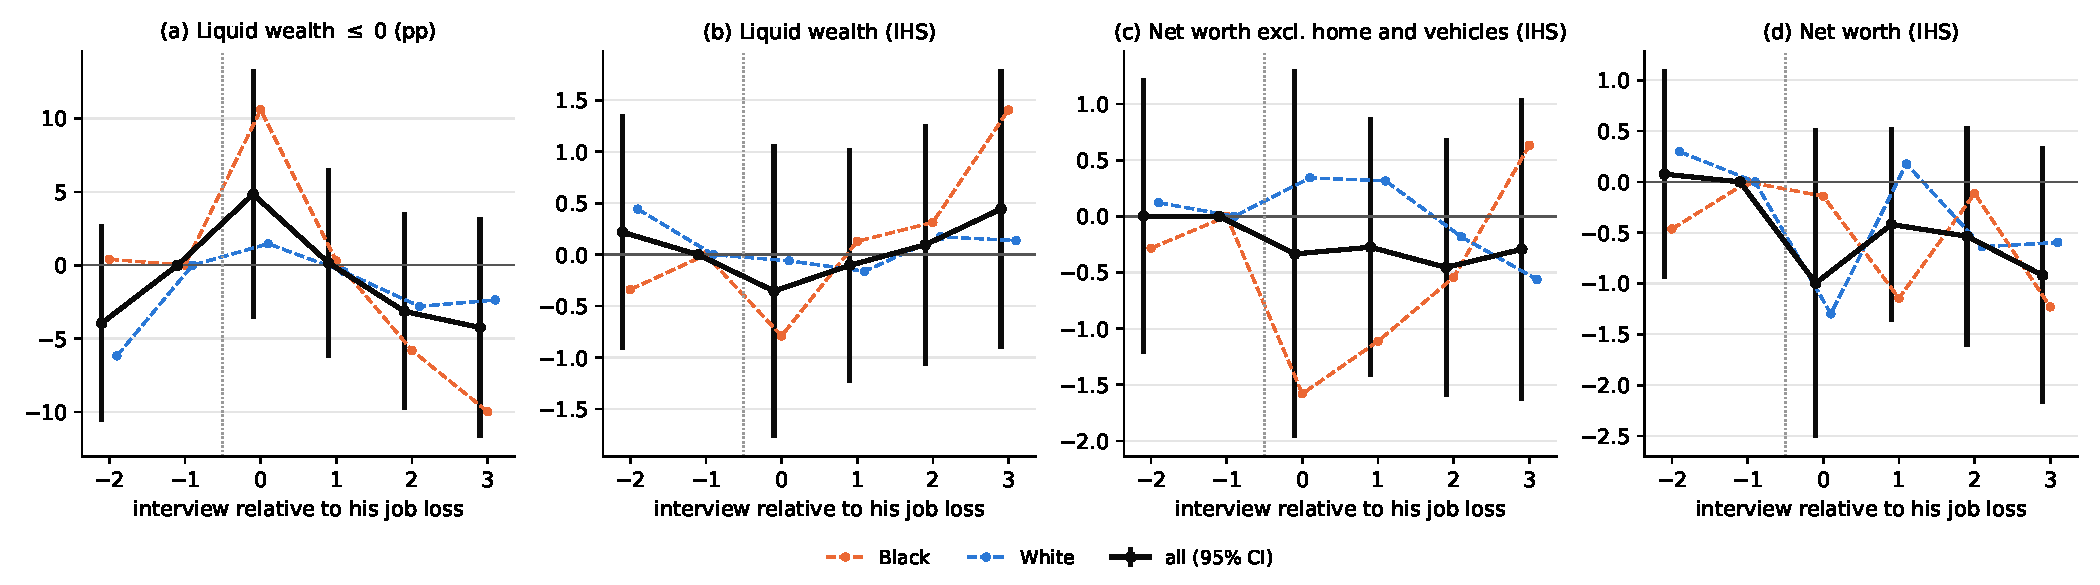
\includegraphics[width=\textwidth]{fig_psid_wealth_event.pdf}
\caption{Wealth around the husband's displacement (PSID wealth waves 1999--2019)}\label{fig:wealth_event}
\begin{minipage}{0.95\textwidth}\footnotesize Stacked event study of the husband's first displacement (closure,
layoff or firing) in 2000--2018, by wealth interview relative to the job-end year (reference: the last interview
before it; interview bins as in Figure~\ref{fig:consumption}), for husbands displaced alone (wife not displaced in the
three years around his job loss), against couples without a displacement; married couples with the wife aged 25--59;
father $\times$ stack and wave $\times$ stack fixed effects; 95\% confidence intervals for all couples clustered by
1968 family (473 displaced husbands, 51 of them with a joint loss estimated separately, 15{,}741 control stacks);
dashed lines: Black and White couples. (a) Liquid wealth (checking and savings, bonds, stocks, minus unsecured debt)
of zero or less, in points; (b)--(d) inverse hyperbolic sine of liquid wealth, of net worth excluding home equity and
vehicles, and of net worth, in 2000 dollars. Means over the first three interviews after the job loss: (a)
$-2.4$ (s.e.\ 3.0, $p=0.41$); (b) $0.15$ (0.53, $p=0.78$); (c) $-0.34$ (0.52, $p=0.51$); (d) $-0.62$ (0.48,
$p=0.19$). At the last interview before the loss, 59.5\% of the displaced husbands' families hold liquid wealth of
zero or less. Unsecured debt is netted in liquid wealth and not shown separately. Code:
\texttt{47.PSIDConsumptionEvent.py --wealth} with the definitions of \texttt{77.WealthDefinitions.py}
(\texttt{output/psid\_wealth\_event.csv}).\end{minipage}
\end{figure}

\section{Robustness of the Joint Job Loss}\label{app:robust}

This appendix documents the checks summarised in Section~\ref{sec:jointloss}: the CPS monthly checks on reporting,
temporary layoffs, the season, persistence, class of worker, a common employer and attrition; the replication in the
Displaced Worker Supplement; and the replication and the added-worker path in the SIPP.

\subsection{The CPS monthly checks}

Three features of the CPS could produce a joint job loss that is not one: one household member usually reports for
both spouses, half of the husbands' job losses are temporary layoffs, and some jobs end with the season or the school
year. None of them accounts for the fact; Table~\ref{tab:cps_checks} reports the estimates.\footnote{Linear probability models with state $\times$ month fixed effects,
standard errors clustered by household; the respondent identifiers (PUSLFPRX, HURESPLI) are matched for 99.6\% of
couple-months. Code: \texttt{IGE/37.CPSJointLossChecks.py} (\texttt{output/cps\_joint\_loss\_checks.md}).}

\emph{Who reports.} The excess is 3.8 points when the wife reports for herself and the husband's job loss is reported by
proxy, and 3.8 points in the reverse case; the difference is 0.0003 ($p=0.936$), and it is the same when the same person
reports in both months. Couples in which a third household member reports for both spouses (4\% of couples) show a
larger excess (0.093$^{***}$); excluding them leaves 3.8 points. Couples in which both spouses report for themselves
cannot be formed, because the CPS takes one respondent per household and month.

\emph{Temporary layoffs, the season and persistence.} Excluding the husband's temporary layoffs, the excess is 2.7
points (0.027$^{***}$); excluding the wife's as well, 2.6 points, on a base of 0.23\%, so the wife's risk is 14 times the
base. A temporary layoff of the husband followed by a permanent job loss of the wife adds only 0.4 points. Temporary
layoffs therefore account for about a third of the headline excess. Excluding June to September leaves 3.7 points, and
excluding the pandemic years 3.5 points. When both spouses are still unemployed two months later, the excess is 2.5
points (0.025$^{***}$) on a base of 0.20\%. The strictest version---both spouses still unemployed two months later, the
husband's loss not a temporary layoff, outside June to September and outside 2020--21---gives 1.6 points
(0.016$^{***}$) on a base of 0.17\%: a joint permanent job loss is about 13 times as likely in the month the husband loses
his job as in other months. The excess is positive in all ten major industries. In education and health it is large
overall (0.091$^{***}$) but 2.0 points for the husband's permanent losses, consistent with school-year layoffs; couples
who both work for government or are both self-employed show the largest excess (0.153$^{***}$ and 0.159$^{***}$), the
latter likely family businesses, and couples who both work in the private sector show 3.0 points for the husband's
permanent losses.

\emph{A common employer.} The public CPS has no employer identifier. The tightest proxy, couples in the same detailed
industry, the same detailed occupation and the same class of worker (6.3\% of couples), shows a joint-loss probability
of 35.7\% (excess 0.337$^{***}$) and accounts for 35\% of the excess; all other couples show 2.6 points. If 10--12\% of
dual-earner couples work at the same establishment \citep{hyatt2019coworking}, the excess requires a joint-loss
probability of 21--41\% among them, depending on the excess elsewhere. A shared employer plausibly carries a third to a
half of the excess. Couples observed in all four months of the rotation show 3.8 points, so attrition after a job loss
does not create the excess.

\begin{table}[!htbp]
\centering
\caption{Robustness of the same-month joint job loss (CPS basic monthly, 1994--2023)}
\label{tab:cps_checks}
\resizebox{\ifdim\width>\textwidth\textwidth\else\width\fi}{!}{%
\resizebox*{!}{\ifdim\totalheight>0.78\textheight 0.78\textheight\else\totalheight\fi}{%
\begin{tabular}{lccccc}
\toprule
Sample & \begin{tabular}[b]{@{}c@{}}Wife loses\\her job\end{tabular} & \begin{tabular}[b]{@{}c@{}}Wife loses her job,\\excluding 2020--21\end{tabular} & \begin{tabular}[b]{@{}c@{}}Wife's loss not a\\temporary layoff\end{tabular} & \begin{tabular}[b]{@{}c@{}}Wife still\\unemployed at $t+2$\end{tabular} & \begin{tabular}[b]{@{}c@{}}Base rate,\\\% a month\end{tabular} \\
 & (1) & (2) & (3) & (4) & (5) \\
\midrule
\multicolumn{6}{l}{\textit{A. Who reports (month of the husband's job loss)}} \\
All couples & $0.040^{***}$ & $0.035^{***}$ &  &  & 0.54 \\
 & (0.002) & (0.001) &  &  & \\
Wife reports for herself, husband by proxy & $0.038^{***}$ & $0.034^{***}$ &  &  & 0.60 \\
 & (0.002) & (0.002) &  &  & \\
\quad and the wife reports his job loss & $0.039^{***}$ & $0.034^{***}$ &  &  & 0.60 \\
 & (0.002) & (0.002) &  &  & \\
Husband reports for himself, wife by proxy & $0.038^{***}$ & $0.032^{***}$ &  &  & 0.47 \\
 & (0.002) & (0.002) &  &  & \\
\quad and the husband reports her job loss & $0.039^{***}$ & $0.032^{***}$ &  &  & 0.47 \\
 & (0.002) & (0.002) &  &  & \\
Wife self, husband proxy in both months & $0.037^{***}$ & $0.031^{***}$ &  &  & 0.59 \\
 & (0.002) & (0.002) &  &  & \\
Husband self, wife proxy in both months & $0.037^{***}$ & $0.030^{***}$ &  &  & 0.46 \\
 & (0.003) & (0.002) &  &  & \\
A third member reports both & $0.093^{***}$ & $0.084^{***}$ &  &  & 0.54 \\
 & (0.010) & (0.010) &  &  & \\
Third-member reports excluded & $0.038^{***}$ & $0.033^{***}$ &  &  & 0.54 \\
 & (0.002) & (0.001) &  &  & \\
\addlinespace
\multicolumn{6}{l}{\textit{B. Temporary layoffs and the season}} \\
All husband job losses & $0.040^{***}$ & $0.035^{***}$ & $0.015^{***}$ & $0.015^{***}$ & 0.54 \\
 & (0.002) & (0.001) & (0.001) & (0.001) & \\
His loss not a temporary layoff & $0.027^{***}$ & $0.027^{***}$ & $0.026^{***}$ & $0.012^{***}$ & 0.54 \\
 & (0.002) & (0.002) & (0.002) & (0.001) & \\
His loss a temporary layoff & $0.054^{***}$ & $0.044^{***}$ & $0.004^{***}$ & $0.017^{***}$ & 0.54 \\
 & (0.002) & (0.002) & (0.001) & (0.002) & \\
Not June--September & $0.037^{***}$ & $0.031^{***}$ & $0.015^{***}$ & $0.015^{***}$ & 0.48 \\
 & (0.002) & (0.002) & (0.001) & (0.001) & \\
Not a temporary layoff, not June--September & $0.026^{***}$ & $0.025^{***}$ & $0.025^{***}$ & $0.012^{***}$ & 0.48 \\
 & (0.002) & (0.002) & (0.002) & (0.002) & \\
\addlinespace
\multicolumn{6}{l}{\textit{C. Persistent job losses (both observed two months later)}} \\
All husband job losses & $0.038^{***}$ & $0.034^{***}$ & $0.014^{***}$ & $0.015^{***}$ & 0.54 \\
 & (0.002) & (0.002) & (0.001) & (0.001) & \\
His loss persistent & $0.033^{***}$ & $0.028^{***}$ & $0.017^{***}$ & $0.025^{***}$ & 0.54 \\
 & (0.003) & (0.002) & (0.002) & (0.002) & \\
Persistent, not a temporary layoff & $0.027^{***}$ & $0.026^{***}$ & $0.025^{***}$ & $0.018^{***}$ & 0.54 \\
 & (0.003) & (0.003) & (0.003) & (0.002) & \\
Persistent, not a temporary layoff, not June--September & $0.028^{***}$ & $0.026^{***}$ & $0.026^{***}$ & $0.017^{***}$ & 0.47 \\
 & (0.004) & (0.004) & (0.003) & (0.003) & \\
\addlinespace
\multicolumn{6}{l}{\textit{D. Class of worker}} \\
Both private & $0.041^{***}$ & $0.036^{***}$ & $0.017^{***}$ & $0.017^{***}$ & 0.59 \\
 & (0.002) & (0.002) & (0.001) & (0.002) & \\
Both private, his loss not a temporary layoff & $0.030^{***}$ & $0.030^{***}$ & $0.029^{***}$ & $0.015^{***}$ & 0.59 \\
 & (0.002) & (0.002) & (0.002) & (0.002) & \\
Both government & $0.153^{***}$ & $0.156^{***}$ & $0.013^{**}$ & $0.040^{***}$ & 0.38 \\
 & (0.016) & (0.017) & (0.006) & (0.010) & \\
Both self-employed & $0.159^{***}$ & $0.142^{***}$ & $0.073^{***}$ & $0.043^{***}$ & 0.30 \\
 & (0.016) & (0.017) & (0.013) & (0.012) & \\
Husband private, wife government & $0.013^{***}$ & $0.007^{***}$ & $0.002^{*}$ & $0.004^{**}$ & 0.60 \\
 & (0.003) & (0.002) & (0.001) & (0.002) & \\
Husband government, wife private & $0.027^{***}$ & $0.024^{***}$ & $0.008^{**}$ & $0.006$ & 0.46 \\
 & (0.007) & (0.006) & (0.004) & (0.004) & \\
\addlinespace
\multicolumn{6}{l}{\textit{E. Shared workplace}} \\
Same major industry & $0.166^{***}$ &  &  &  & 0.44 \\
 & (0.007) &  &  &  & \\
Same detailed industry & $0.211^{***}$ &  &  &  & 0.41 \\
 & (0.009) &  &  &  & \\
Same detailed industry and occupation & $0.315^{***}$ &  &  &  & 0.41 \\
 & (0.014) &  &  &  & \\
Same detailed industry, occupation and class & $0.337^{***}$ &  &  &  & 0.41 \\
 & (0.015) &  &  &  & \\
All other couples & $0.026^{***}$ &  &  &  & 0.55 \\
 & (0.001) &  &  &  & \\
\addlinespace
\multicolumn{6}{l}{\textit{F. Attrition}} \\
Couples observed in all four months & $0.038^{***}$ & $0.033^{***}$ &  &  & 0.54 \\
 & (0.002) & (0.002) &  &  & \\
Couples not observed in all four months & $0.052^{***}$ & $0.045^{***}$ &  &  & 0.57 \\
 & (0.004) & (0.004) &  &  & \\
\bottomrule
\end{tabular}}}
\par\smallskip
\begin{minipage}{\textwidth}\footnotesize \textit{Notes:} Each cell is the coefficient on the husband losing his job in a linear probability model of the outcome in the column header, among married couples in which both spouses work in the previous month, with state $\times$ month fixed effects; standard errors clustered by household (state clustering gives the same significance). Column (5): the wife's job-loss rate when the husband does not lose his job. A job loser is unemployed after a layoff, a job loss or the end of a temporary job, having been employed the month before. Persistent: still unemployed two months later. Panel A: labor force information collected from the person (self) or from another household member (proxy); couples in which both spouses report for themselves cannot be formed because the CPS takes one respondent per household and month. $^{***}$ $p<0.01$, $^{**}$ $p<0.05$, $^{*}$ $p<0.1$. Source: \texttt{IGE/37.CPSJointLossChecks.py} (\texttt{output/cps\_joint\_loss\_checks.csv}); table built by \texttt{IGE/48.PaperATables.py}.\end{minipage}
\end{table}


\subsection{The Displaced Worker Supplement}

The CPS Displaced Worker Supplement, fielded every two years from 1984 to 2024, asks every adult whether he or she lost
a job in the last three years because the plant closed or moved, there was insufficient work or the position was
abolished, and in which year. It combines the reason-based measure of the PSID with the sample size of the CPS: 417,269
couples in which both spouses answer the supplement, 24,038 displaced husbands and 1,968 couples in which both were
displaced.\footnote{IPUMS CPS, 21 supplements; couples aged 20--64 naming each other as spouse; the 1984--1992 five-year
window and reasons are harmonised to the later three-year definition. Linear probability models with state $\times$
survey-year fixed effects and controls for both spouses' age, education and race; standard errors clustered by
household (state clustering gives the same significance). Code: \texttt{IGE/39.CPSDisplacedWorkers.py}
(\texttt{output/cps\_dws\_joint\_loss.md}).} A wife was displaced in the three-year window in 8.2\% of couples in which
the husband was displaced and in 3.3\% of the others (an excess of 4.4 points, 0.044$^{***}$, s.e.\ 0.002), and in the same
calendar year in 4.7\% against 1.1\% (0.033$^{***}$, s.e.\ 0.001), while a displacement of the husband in another year of
the window adds only 0.5 points. Both spouses lost their jobs to plant closings 4.7 times as often as independent
closings would imply (0.046$^{***}$), and 9.8 times within the same year. Joint displacements share the lost job's
detailed industry in 29\% of cases, 41\% within the same year and 68\% for same-year joint closings, against 1.3\% for
randomly paired spouses; the excess rises by 40 points when the spouses worked in the same detailed industry
(0.399$^{***}$). The tetrachoric correlation of the spouses' displacements is 0.26 within the same year (0.35 for plant
closings), close to the PSID's 0.24. The excess is the same for Black and White couples ($-0.001$, $p=0.894$), in
1984--1998 and 2000--2024 (difference 0.004, $p=0.252$) and in recession and expansion windows (0.004, $p=0.305$). After
a joint displacement neither spouse works at the survey more often: 8.8 points more (0.088$^{***}$) on a base of 9.3\%.

\subsection{The SIPP}

The public-use SIPP core files of the 2004 (waves 1--12, 2003--2007), 2008 (waves 1--16, 2008--2013) and 2014
(waves 1--4, 2013--2016) panels give 1,595,445 couple-months of 50,692 married couples aged 20--60 who name each other
as spouse. An involuntary separation is an employer job that ends for layoff or slack work, closure, discharge or the end
of a temporary job, from the reason-for-leaving item. The public employer numbers are person-specific, so a shared
employer cannot be identified.\footnote{Linear probability models among couples in which both spouses were employed the
month before, with state $\times$ panel $\times$ rotation $\times$ month fixed effects; standard errors clustered by
household. Code: \texttt{IGE/40.SIPPJointLoss.py} (\texttt{output/sipp\_joint\_loss.md}).}

The wife's involuntary separation rate is 3.28\% in the month in which her husband separates and 0.43\% otherwise
(ratio 7.7; excess 0.027$^{***}$, s.e.\ 0.003, on 4,479 husbands' separations and 143 joint events); requiring that she has
no job the next month, as in the CPS, gives a ratio of 13.1 (excess 0.028$^{***}$). Over twelve months the ratio is 2.4,
against 2.6 in the PSID's couple-years. The excess holds outside the interview seam (0.027$^{***}$), for couples in which
both spouses report for themselves (0.019$^{***}$), without imputed records (0.028$^{***}$), in each panel (2004
0.036$^{***}$, 2008 0.022$^{***}$, 2014 0.028$^{***}$) and outside the 2008--09 recession (0.030$^{***}$). It rises by 22
points when the spouses share a detailed industry (0.220$^{***}$), where 23.9\% of wives separate in their husband's
month, and by 11 points in the same major industry. The timing matches the CPS: the excess is 2.6 points in the month of
the husband's separation, 0.4 points in the month before, and spread thinly over the months around it.

The SIPP differs from the CPS and the Displaced Worker Supplement in one respect: for Black husbands the same-month
excess is 0.007 ($p=0.123$) against 0.027$^{***}$ for White husbands (difference $-0.017^{***}$), on six joint events among
435 Black husbands' separations; over the month of the separation and the following twelve the excess is similar
(Black 0.050$^{***}$, White 0.063$^{***}$). With so few events this difference is fragile.

The SIPP also traces the wife's response month by month for three years. Among wives with no job the month before, the
probability of looking for work rises at once (0.053$^{***}$) and fades over three years (0.013, $p=0.246$ at 36 months),
while employment builds up slowly: 0.019$^{***}$ in the month of the husband's separation, 0.037$^{***}$ a month later and
0.054$^{***}$ after six months, and still 0.044$^{***}$ after 24 months. These wives were more often employed and looking
six months earlier, so some had recently lost or left jobs; among wives with no job in any of the six previous months,
employment rises from 0.015$^{***}$ to 0.045$^{***}$ after six months. Wives who were working see their employment fall by
3.4 points a month after the husband's separation, about half of it their own job loss, so the net change in all wives'
employment is about zero for a year ($-0.007^{**}$ after one month, 0.006, $p=0.297$, after twelve); leaving out the wives
who lost their own job it is 0.011$^{*}$ after twelve months and 0.020$^{**}$ after 24.

\section{Reconciliation with Blundell, Pistaferri and Saporta-Eksten (2016)}\label{app:bps}

This appendix reports the replication of \citet{blundell2016consumption} and the exercises summarised in
Section~\ref{sec:literature}. Their do-files are run on their constructed PSID panel for 1999--2009; copies of the
do-files, with every edit marked and listed, are in \texttt{IGE/bps\_reconciliation/code/}, and every number is in
\texttt{IGE/bps\_reconciliation/bps\_reconciliation.md} and \texttt{.csv}.\footnote{The 1999 early-release income file
needed to rebuild their panel from the raw PSID is not public, so the replication starts from their constructed panel;
their sample and preparation code reproduce their estimation file exactly (10,479 household-years). The 1997 immigrant
refresher, which their footnote 15 says is excluded, is kept by their code; dropping it changes nothing material
(family share 0.626). Bootstrap standard errors use 50 replications against their 200.}

Table~\ref{tab:bps_relax} reproduces their estimates in column 1---the wage process of their Table 3, the preference
parameters of their Table 4, the elasticities of their Table 5 and the insurance chain (7.09, 6.33, 5.79, 3.88 and 3.16\%,
a split of 19.4\% government, 62.3\% family labor supply and 18.3\% savings, and 70.6\% government among
food-stamp-eligible households)---and relaxes one restriction at a time in the other columns. Without both trims, or
with all relaxations together, the estimator is degenerate. Table~\ref{tab:bps_attrition} shows where the displaced
couples leave their sample. Table~\ref{tab:bps_event} reports the event study of single and joint displacements on their
residuals. Two further results: their extensive-margin added-worker response ($\theta_1=-0.168^{*}$) consists of entries
into work ($-0.159^{**}$) rather than exits ($-0.009$); and separations follow a wife's displacement 2.9 percentage points
more often ($p=0.033$), while a husband's displacement raises them by 1.0 point ($p=0.26$), and ending a couple's record
only when the spouse's identity changes alters nothing.

\begin{table}[!htbp]
\centering
\caption{Blundell, Pistaferri and Saporta-Eksten (2016) under their restrictions and without them}
\label{tab:bps_relax}
\resizebox{\ifdim\width>\textwidth\textwidth\else\width\fi}{!}{%
\begin{tabular}{lcccccccc}
\toprule
Parameter & \begin{tabular}[b]{@{}c@{}}Baseline\\(their\\sample)\end{tabular} & \begin{tabular}[b]{@{}c@{}}Drop only\\the year\\without work\end{tabular} & \begin{tabular}[b]{@{}c@{}}No\\status\\controls\end{tabular} & \begin{tabular}[b]{@{}c@{}}No jump\\trim\end{tabular} & \begin{tabular}[b]{@{}c@{}}No\\minimum-\\wage trim\end{tabular} & \begin{tabular}[b]{@{}c@{}}Low-income\\sample in\end{tabular} & \begin{tabular}[b]{@{}c@{}}Low-income\\sample in,\\weighted\end{tabular} & \begin{tabular}[b]{@{}c@{}}White\\couples\\(low-income in)\end{tabular} \\
 & (1) & (2) & (3) & (4) & (5) & (6) & (7) & (8) \\
\midrule
\multicolumn{9}{l}{\textit{Wage process}} \\
Cov., transitory wage shocks & $0.006^{**}$ & $0.006^{**}$ & $0.006^{**}$ & $0.004$ & $0.007^{**}$ & $0.006^{**}$ & $0.005^{*}$ & $0.007^{**}$ \\
 & (0.003) & (0.003) & (0.003) & (0.004) & (0.003) & (0.003) & (0.003) & (0.003) \\
Cov., permanent wage shocks & $0.003$ & $0.002$ & $0.003$ & $0.004$ & $0.001$ & $0.003$ & $0.003$ & $0.003$ \\
 & (0.002) & (0.002) & (0.002) & (0.002) & (0.003) & (0.002) & (0.002) & (0.003) \\
\quad correlation, transitory & $0.31$ & $0.29$ & $0.31$ & $0.10$ & $0.24$ & $0.26$ & $0.21$ & $0.28$ \\
\quad correlation, permanent & $0.08$ & $0.07$ & $0.08$ & $0.16$ & $0.02$ & $0.09$ & $0.10$ & $0.10$ \\
\addlinespace
\multicolumn{9}{l}{\textit{Preferences and elasticities}} \\
$E(\pi)$, partial insurance & $0.150^{***}$ & $0.152^{***}$ & $0.150^{***}$ & $0.151^{***}$ & $0.154^{***}$ & $0.140^{***}$ & $0.140^{***}$ & $0.158^{***}$ \\
 & (0.004) & (0.004) & (0.004) & (0.004) & (0.006) & (0.003) & (0.003) & (0.004) \\
$\eta_{c,p}$ & $0.418^{**}$ & $0.516^{***}$ & $0.430^{***}$ & $0.079$ & $0.259^{***}$ & $0.311$ & $0.267^{*}$ & $0.566$ \\
 & (0.174) & (0.173) & (0.163) & (0.069) & (0.081) & (0.197) & (0.148) & (0.394) \\
$\eta_{h_1,w_1}$ & $0.681^{***}$ & $0.647^{***}$ & $0.700^{***}$ & $0.508^{***}$ & $0.651^{**}$ & $0.719^{***}$ & $0.704^{***}$ & $0.420^{***}$ \\
 & (0.133) & (0.117) & (0.139) & (0.108) & (0.256) & (0.175) & (0.197) & (0.136) \\
$\eta_{h_2,w_2}$ & $0.958^{***}$ & $0.957^{***}$ & $1.009^{***}$ & $0.840^{***}$ & $0.640^{***}$ & $0.846^{***}$ & $0.932^{***}$ & $1.053^{***}$ \\
 & (0.225) & (0.189) & (0.233) & (0.244) & (0.113) & (0.161) & (0.241) & (0.303) \\
Wife's hours / husband's permanent wage & $-0.752^{***}$ & $-0.691^{***}$ & $-0.773^{***}$ & $-1.358^{***}$ & $-0.647^{***}$ & $-0.768^{***}$ & $-0.849^{***}$ & $-0.764^{***}$ \\
 & (0.098) & (0.119) & (0.093) & (0.227) & (0.136) & (0.180) & (0.172) & (0.208) \\
Consumption / husband's permanent wage & $0.316^{***}$ & $0.347^{***}$ & $0.318^{***}$ & $0.028$ & $0.245^{***}$ & $0.279^{***}$ & $0.246^{***}$ & $0.383^{***}$ \\
 & (0.057) & (0.047) & (0.069) & (0.101) & (0.051) & (0.091) & (0.070) & (0.073) \\
\addlinespace
\multicolumn{9}{l}{\textit{Insurance against a permanent fall in the husband's wage}} \\
Share of insurance: government & $0.194^{***}$ & $0.215^{***}$ & $0.194^{***}$ & $0.112^{***}$ & $0.171^{***}$ & $0.179^{***}$ & $0.162^{***}$ & $0.215^{***}$ \\
 & (0.031) & (0.030) & (0.035) & (0.020) & (0.021) & (0.042) & (0.028) & (0.052) \\
Share of insurance: family labor supply & $0.623^{***}$ & $0.561^{***}$ & $0.621^{***}$ & $0.875^{***}$ & $0.700^{***}$ & $0.678^{***}$ & $0.700^{***}$ & $0.517^{***}$ \\
 & (0.093) & (0.086) & (0.099) & (0.063) & (0.054) & (0.110) & (0.081) & (0.155) \\
Share of insurance: savings & $0.183^{***}$ & $0.224^{***}$ & $0.185^{***}$ & $0.014$ & $0.129^{***}$ & $0.143^{**}$ & $0.138^{**}$ & $0.268^{***}$ \\
 & (0.060) & (0.057) & (0.064) & (0.043) & (0.035) & (0.068) & (0.054) & (0.103) \\
Outside insurance $\beta$ & $-0.138$ & $-0.029$ & $-0.105$ & $-1.782$ & $0.252^{*}$ & $-0.273$ & $0.059$ & $-0.197$ \\
 & (0.213) & (0.270) & (0.188) & (3.224) & (0.145) & (0.307) & (0.660) & (0.344) \\
Observations & 7,295 & 7,642 & 7,295 & 7,341 & 7,396 & 8,795 & 8,729 & 5,920 \\
\bottomrule
\end{tabular}}
\par\smallskip
\begin{minipage}{\textwidth}\footnotesize \textit{Notes:} Their code run on their constructed PSID panel, 1999--2009. Column (1) reproduces their Tables 3--5 and their insurance accounting. Each further column relaxes one restriction: (2) drops only the year in which the husband has no hours or earnings instead of his whole record; (3) removes both spouses' employment-status controls from the residual regressions; (4) removes the trim of years of collapse and recovery; (5) removes the trim of wages below half the state minimum wage; (6)--(7) include the PSID's low-income sample; (8) White couples with the low-income sample. Wage process: GMM standard errors clustered by household; preferences, elasticities and insurance: block bootstrap over households (50 replications). $^{***}$ $p<0.01$, $^{**}$ $p<0.05$, $^{*}$ $p<0.1$. Source: \texttt{IGE/bps\_reconciliation/} (\texttt{bps\_reconciliation.csv}); table built by \texttt{IGE/48.PaperATables.py}.\end{minipage}
\end{table}

\begin{table}[!htbp]
\centering
\caption{Where the displaced couples leave the sample of Blundell, Pistaferri and Saporta-Eksten (2016)}
\label{tab:bps_attrition}
\resizebox{\ifdim\width>\textwidth\textwidth\else\width\fi}{!}{%
\begin{tabular}{lcccc}
\toprule
Step & \begin{tabular}[b]{@{}c@{}}Couple-\\years\end{tabular} & \begin{tabular}[b]{@{}c@{}}Husband\\displaced\end{tabular} & \begin{tabular}[b]{@{}c@{}}Wife\\displaced\end{tabular} & \begin{tabular}[b]{@{}c@{}}Both\\displaced\end{tabular} \\
 & (1) & (2) & (3) & (4) \\
\midrule
Married couples, husband 30--57, SRC and low-income samples & 14,327 & 692 & 480 & 57 \\
Drop the year of a change in family composition & 13,876 & 658 & 460 & 52 \\
Drop if not married & 13,876 & 658 & 460 & 52 \\
Drop if state missing & 13,811 & 654 & 456 & 51 \\
Drop female heads, age always missing & 13,811 & 654 & 456 & 51 \\
Drop net worth of \$20 million or more & 13,802 & 654 & 456 & 51 \\
Keep ages 30--57 & 13,767 & 653 & 455 & 51 \\
Drop the low-income (SEO) sample & 10,857 & 488 & 345 & 37 \\
Drop if education missing & 10,157 & 449 & 317 & 33 \\
Merge minimum wages and prices & 10,157 & 449 & 317 & 33 \\
Drop husbands with any year without work (estimation file) & 9,148 & 404 & 283 & 28 \\
Keep rows with a husband's wage-growth moment & 6,372 & 293 & 186 & 17 \\
Keep rows with both spouses' wage-growth moments & 4,762 & 208 & 160 & 16 \\
\bottomrule
\end{tabular}}
\par\smallskip
\begin{minipage}{\textwidth}\footnotesize \textit{Notes:} Universe: married couples with husbands aged 30--57 in the PSID's SRC and low-income samples, waves 1999--2009. Their restrictions applied in their order; each row counts the couple-years left after the step. The last rows keep couple-years with a husband's wage-growth moment and with both spouses' wage-growth moments. Source: \texttt{IGE/bps\_reconciliation/} (\texttt{bps\_reconciliation.csv}); table built by \texttt{IGE/48.PaperATables.py}.\end{minipage}
\end{table}

\begin{table}[!htbp]
\centering
\caption{Single and joint displacements in the panel of Blundell, Pistaferri and Saporta-Eksten (2016)}
\label{tab:bps_event}
\resizebox{\ifdim\width>\textwidth\textwidth\else\width\fi}{!}{%
\begin{tabular}{lccc}
\toprule
 & \begin{tabular}[b]{@{}c@{}}Their\\sample\end{tabular} & \begin{tabular}[b]{@{}c@{}}Low-income\\sample in\end{tabular} & \begin{tabular}[b]{@{}c@{}}All\\relaxations\end{tabular} \\
 & (1) & (2) & (3) \\
\midrule
\multicolumn{4}{l}{\textit{Consumption residual, interval of the displacement}} \\
Husband displaced alone & $-0.022$ & $-0.019$ & $-0.017$ \\
 & (0.020) & (0.019) & (0.019) \\
Both displaced & $0.049$ & $0.047$ & $-0.009$ \\
 & (0.087) & (0.072) & (0.073) \\
Both $-$ husband alone & $0.071$ & $0.066$ & $0.008$ \\
 & (0.089) & (0.074) & (0.075) \\
\quad joint events & 17 & 23 & 25 \\
\addlinespace
\multicolumn{4}{l}{\textit{Consumption residual, next interval}} \\
Husband displaced alone & $0.009$ & $0.028$ & $0.033^{*}$ \\
 & (0.020) & (0.019) & (0.018) \\
Both displaced & $-0.062$ & $-0.110^{*}$ & $-0.101^{*}$ \\
 & (0.050) & (0.059) & (0.056) \\
Both $-$ husband alone & $-0.071$ & $-0.138^{**}$ & $-0.134^{**}$ \\
 & (0.054) & (0.062) & (0.059) \\
\quad joint events & 18 & 21 & 22 \\
\addlinespace
\multicolumn{4}{l}{\textit{Husband's earnings residual, interval of the displacement}} \\
Husband displaced alone & $-0.123^{***}$ & $-0.105^{***}$ & $-0.145^{***}$ \\
 & (0.040) & (0.037) & (0.042) \\
Both displaced & $-0.335^{*}$ & $-0.356^{**}$ & $-0.337^{**}$ \\
 & (0.178) & (0.140) & (0.142) \\
\addlinespace
\multicolumn{4}{l}{\textit{Wife's earnings, arc change, interval of the displacement}} \\
Both $-$ husband alone & $-0.438^{***}$ & $-0.377^{***}$ & $-0.377^{**}$ \\
 & (0.138) & (0.117) & (0.147) \\
\bottomrule
\end{tabular}}
\par\smallskip
\begin{minipage}{\textwidth}\footnotesize \textit{Notes:} Biennial event study on their residuals (consumption and earnings growth net of their observables), PSID 1999--2009, with the PSID reason-for-job-end flags of Section~\ref{sec:data}: husband displaced alone, both spouses displaced, relative to couples without a displacement. Interval of the displacement: the two-year change that contains the job-end year; next interval: the following two-year change. Wife's earnings: arc change including zeros. Column (3) applies all relaxations of Table~\ref{tab:bps_relax} that leave the estimator defined. Standard errors clustered by household. Associations, with few joint events. $^{***}$ $p<0.01$, $^{**}$ $p<0.05$, $^{*}$ $p<0.1$. Source: \texttt{IGE/bps\_reconciliation/} (\texttt{bps\_reconciliation.csv}); table built by \texttt{IGE/48.PaperATables.py}.\end{minipage}
\end{table}


\section{Designs That Did Not Identify Their Target}\label{app:designs}

This appendix reports three designs that were run and did not identify what they were meant to, so that the reader
can see every test behind the argument.

\paragraph{Gender-specific labor-demand shocks at a birth.} To separate the mother's re-employment friction from the
husband's risk, I built shift-share (Bartik) shocks to employment in women's and men's industries by state from the CPS
Outgoing Rotation Groups (1979--2019, 16 sectors). In a split-sample test, the women's shock does not predict women's
state employment growth ($-0.25$, s.e.\ 0.18), while the men's shock predicts men's (0.24, s.e.\ 0.11). With only 16
sectors, the variation left after state and year fixed effects is small, and the leave-one-out construction adds
mechanical noise from small CPS cells. The women's shock is therefore not used. Code: \texttt{IGE/8a.StateShocks.py},
\texttt{IGE/8.FirstStage.py}.

\paragraph{The Family and Medical Leave Act.} I compared births to NLSY79 mothers eligible for job-protected leave
(employer of 50 or more at the location, 12 months of tenure, 1,250 hours) before and after August 1993. The
difference-in-differences estimate on returning to the pre-birth employer within 12 weeks is $-0.073$ (s.e.\ 0.034), and
the estimates at 26 and 52 weeks are not significant. The design is weak: eligible mothers were already near the
ceiling of returning (0.88--0.93), the 1994 redesign of the NLSY79 coincides with the post period and changes the
measured frequency of breaks, and returning within 12 weeks mechanically misses mothers who took the full 12 weeks of
leave. Code: \texttt{IGE/12.FMLA.py}.

\paragraph{State-by-sector shocks to husbands.} Employment growth in the husband's sector within his state has no
first stage on the husband's hours or earnings (F below 1), even with split-sample instruments, so only national sector
shocks are used in Appendix~\ref{sec:birthshocks}. Code: \texttt{IGE/18.HusbandIndustryShocks.py}.


\end{document}
